\documentclass[a4paper,11pt,titlepage,twoside]{article}
\usepackage[utf8]{inputenc}

\newcommand{\Language}{CZ}
%varianty {EN} english
%         {CZ} czech
\newcommand{\Thesis}{M}
%varianty {B} bakalářská práce
%         {M} diplomová práce
%         {D} dizertační práce
\newcommand{\Faculty}{Fakulta elektrotechnická}
\newcommand{\Department}{Kybernetika a robotika}
\newcommand{\Author}{Jakub Drápela}
\newcommand{\Title}{Automatické odhadování plošek broušeného kamene}
\newcommand{\Date}{Květen 2017}
\newcommand{\Supervisor}{Ing. Vladimír Smutný, Ph.D.}

%% definice pouziteho vzoru %%%%%%%%%%%%%%%%%%%%%%%%%%%%%

\usepackage[left=3.0cm,right=2.4cm,top=3cm,bottom=4cm]{geometry}

	\usepackage{amssymb,amsmath}
	
%%Packages definition
	\usepackage{ifthen}
	
	%% language package
	\ifthenelse{ \equal{\Language}{EN} }{
  		\usepackage[english]{babel}
	}{
  		\usepackage[czech]{babel}
	}
    
	\usepackage{lipsum}		%% lorem ipsum ... 
	\usepackage{fancyhdr}	%% header and footer
	\usepackage[dvips]{graphicx}   %% graphics
	\usepackage{booktabs}   %% tables
	\usepackage[cmyk,table]{xcolor} %% colors
	\usepackage{tikz}		%% diagrams

	\usepackage[font=small,labelfont=bf]{caption}	%% figures
	\usepackage{subcaption}	%% subfigures

	\usepackage{url}		%% web links
	\usepackage{epstopdf}	%% we all know this one
	\usepackage{rotating}
	\usepackage[crop=pdfcrop]{pstool}
    \usepackage[backend=bibtex,style=numeric]{biblatex}
	\usepackage{psfrag}
	\usepackage{epsf} 
	\usepackage{multirow}	
	\usepackage{wrapfig}
	\usepackage[titletoc]{appendix}
	\usepackage{siunitx}
	
	
	\usepackage[absolute]{textpos}	%% for the page with scanned assignment
	
	%% PROSTOR PRO IMPORT UZIVATELSKYCH BALICKU %%%%%%%%%%%%%
%\usepackage[T1]{fontenc}
\usepackage{amsmath}


\usepackage{amsfonts}
\usepackage{amssymb}
%\usepackage{graphicx}

\usepackage{indentfirst}
\usepackage{esvect}
%\setlength{\parindent}{4em} 


\usepackage{enumitem}
\usepackage{textcomp} % to use \textperthousand                                            


% pridano kvuli tabulkam 
\usepackage{array}
\newcolumntype{L}[1]{>{\raggedright\let\newline\\\arraybackslash\hspace{0pt}}m{#1}}
\newcolumntype{C}[1]{>{\centering\let\newline\\\arraybackslash\hspace{0pt}}m{#1}}
\newcolumntype{R}[1]{>{\raggedleft\let\newline\\\arraybackslash\hspace{0pt}}m{#1}}

\DeclareSIUnit\px{px}
\DeclareSIUnit\permille{\text{\textperthousand}}
\DeclareMathOperator*{\argmax}{arg\,max}
\DeclareMathOperator*{\argmin}{arg\,min}
%\makeatletter
%\renewcommand{\@makechapterhead}[1]{%
%\vspace*{20 pt}%
%{\setlength{\parindent}{0pt} \raggedright \normalfont
%\bfseries\Huge\thechapter.\ #1
%\par\nobreak\vspace{20 pt}}}
%\makeatother

%\setcounter{secnumdepth}{3}
%\fontfamily{phs}
%%\selectfont
%\usepackage[backend=bibtex,style=numeric,sortcites]{biblatex}


%%Colors definition
	\definecolor{cvutcolor}{cmyk}{1, 0.43, 0, 0} % CVUT blue
	%\definecolor{cvutcolor}{cmyk}{0, 0.78, 0.78, 0.31} %crimson
	%\definecolor{cvutcolor}{cmyk}{0.31, 0, 1, 0.27} %green
	%\definecolor{cvutcolor}{cmyk}{0, 0.35, 1, 0.11} %gold
	\definecolor{svetlemodra}{cmyk}{0.2, 0.08, 0, 0.1} % CVUT light blue
	\definecolor{svetleseda}{cmyk}{0, 0, 0, 0.13} % CVUT light gray

%%Okraje stranky
	\usepackage{lastpage} %% last page reference
	
%%Measurement definition - for the blue ruler on the first pages
	\newlength{\titlewidth}
	\setlength{\titlewidth}{\textwidth}
	\addtolength{\titlewidth}{-1.7cm}
	\newlength{\heightofhw}

%% LANGUAGE SWITCH %%%%%%%%%%%%%%%%%%%%%%%%%%%%%%%%%%%%%%%%%%%%%%%%%%%%%%%%%%%%%%%%%%%%%%%
\ifthenelse{ \equal{\Language}{EN} }{	
	\AtBeginDocument{\renewcommand{\partname}{\sffamily Part}}
	
	\newcommand{\MySchoolName}{\Large \textsc{Czech\\ Technical\\ University\\ in Prague}}
	\newcommand{\MySupervisorLabel}{Thesis supervisor:}
	\ifthenelse{ \equal{\Thesis}{B} }{
		\newcommand{\MyThesisType}{Bachelor's thesis}
	}{}\ifthenelse{ \equal{\Thesis}{M} }{
		\newcommand{\MyThesisType}{Master's thesis}
	}{}\ifthenelse{ \equal{\Thesis}{D} }{
		\newcommand{\MyThesisType}{Ph.D thesis}
	}{}
}{
	\AtBeginDocument{\renewcommand{\partname}{\sffamily Kapitola}}
	\AtBeginDocument{\renewcommand{\refname}{Literatura}}
	
	\newcommand{\MySchoolName}{\large \textsc{České\\ vysoké\\ učení\\ technické\\ v Praze}}
	\newcommand{\MySupervisorLabel}{Vedoucí práce:}
	\ifthenelse{ \equal{\Thesis}{B} }{
		\newcommand{\MyThesisType}{Bakalářská práce}
	}{}\ifthenelse{ \equal{\Thesis}{M} }{
		\newcommand{\MyThesisType}{Diplomová práce}
	}{}\ifthenelse{ \equal{\Thesis}{D} }{
		\newcommand{\MyThesisType}{Dizertační práce}
	}{}
}

%%%%%%%%%%%%%%%%%%%%%%%%%%%%%%%%%%%%%%%%%%%%%%%%%%%%%%%%%%%%%%%%%%%%%%%%%%%%%%%%%%%%%%%%%%
%% TITLE PAGE %%%%%%%%%%%%%%%%%%%%%%%%%%%%%%%%%%%%%%%%%%%%%%%%%%%%%%%%%%%%%%%%%%%%%%%%%%%%
%%%%%%%%%%%%%%%%%%%%%%%%%%%%%%%%%%%%%%%%%%%%%%%%%%%%%%%%%%%%%%%%%%%%%%%%%%%%%%%%%%%%%%%%%%
\newcommand{\TitlePage}{
	\thispagestyle{empty}
	\parbox{0.7cm}{\color{cvutcolor}\rule{0.35cm}{\textheight}}	%% blue rule
	{\parbox[0][\textheight][t]{\titlewidth}{ 
		\vspace{10pt}  		
		\sffamily 
		
\includegraphics[height=3.1cm]{lev.png}	%% lev cvut
  		\put(10,40){\parbox{8cm}{\MySchoolName}}\\[12pt]

		\textbf{\large 
			\color{cvutcolor} {\Faculty} \\[6pt]
			\color{black} {\Department}
		}\\[3.1cm]	
		\textbf{\large \MyThesisType}\\[-1em]	
		\begin{flushleft}
			%\begin{Huge}
			\fontsize{32pt}{2.5em}
			\selectfont \color{cvutcolor} \textbf{\Title}
			%\end{Huge}
			\\[1em]	
		\end{flushleft}
		\Large \color{black} \textbf{\Author}\\
		\vfill{}
		\textbf{\large \Date} \\
		\textbf{\large \MySupervisorLabel} \Supervisor
	}}
	\newpage
}

%%%%%%%%%%%%%%%%%%%%%%%%%%%%%%%%%%%%%%%%%%%%%%%%%%%%%%%%%%%%%%%%%%%%%%%%%%%%%%%%%%%%%%%%%%
%% PAGESTYLES %%%%%%%%%%%%%%%%%%%%%%%%%%%%%%%%%%%%%%%%%%%%%%%%%%%%%%%%%%%%%%%%%%%%%%%%%%%%
%%%%%%%%%%%%%%%%%%%%%%%%%%%%%%%%%%%%%%%%%%%%%%%%%%%%%%%%%%%%%%%%%%%%%%%%%%%%%%%%%%%%%%%%%%

%%definition of pagestyle - normal text - blue header text, blue line pagenumber 
\fancypagestyle{pagestyle_text}{
	\fancyhead{}
	\fancyfoot{}
	\fancyfoot[RO]{
		\textbf{\thepage$/$\pageref*{LastPage}}
		}
	\renewcommand{\headrulewidth}{0pt}
	\fancyfoot[RE,LO]{}
	\fancyfoot[LE]{
		\textbf{\thepage$/$\pageref*{LastPage}}
		}
	
	\fancyhead[RO]{\color{cvutcolor} \slshape \leftmark}
	\fancyhead[RE]{}
	\fancyhead[LE]{\color{cvutcolor} \slshape \leftmark}
	\fancyhead[LO]{}
	
}

%%definition of pagestyle with part heading - no header text, blue line pagenumber
\fancypagestyle{pagestyle_chapter}{
	\fancyhead{}
	\fancyfoot{}
	\fancyfoot[RO]{
		\textbf{\thepage$/$\pageref*{LastPage}}
		}
	\renewcommand{\headrulewidth}{0pt}
	\fancyfoot[RE,LO]{}
	\fancyfoot[LE]{
		\textbf{\thepage$/$\pageref*{LastPage}}
		}
}

%%definition of pagestyle with vertical blue ruler on the left side
\fancypagestyle{pagestyle_blue_rule}{
	\fancyhead{}
	\fancyfoot{}
	\fancyhead[L]{
		\hspace{-1cm}
		\begin{tikzpicture}
		\color{cvutcolor} \draw [line width=0.35cm] (0,-1) -- (0,-1.06\textheight);
		\end{tikzpicture}
		\vspace{-1.06\textheight}
	}
	\fancyfoot[C]{\thepage \qquad \qquad \qquad}
	\renewcommand{\headrulewidth}{0pt}
}

%%%%%%%%%%%%%%%%%%%%%%%%%%%%%%%%%%%%%%%%%%%%%%%%%%%%%%%%%%%%%%%%%%%%%%%%%%%%%%%%%%%%%%%%%%
%% OTHER OPTIONS %%%%%%%%%%%%%%%%%%%%%%%%%%%%%%%%%%%%%%%%%%%%%%%%%%%%%%%%%%%%%%%%%%%%%%%%%
%%%%%%%%%%%%%%%%%%%%%%%%%%%%%%%%%%%%%%%%%%%%%%%%%%%%%%%%%%%%%%%%%%%%%%%%%%%%%%%%%%%%%%%%%%

%%definition of hyperlinks in the text
%\usepackage[
%	bookmarks=true,
%	hypertexnames=false,
%	breaklinks=true,
%	colorlinks=false,
%	urlcolor=blue,
%	linktoc=section,
%	linkbordercolor={1 0.8 0},
%	citebordercolor={0.36 0.54 0.76}%cyan%{0 0.68 0.84}%{0 0.36 0.72}%{0 1 0}
%]{hyperref}
\definecolor{lgray}{gray}{.9}
  \definecolor{dgreen}{rgb}{0,0.4,0}
  \definecolor{dblue}{rgb}{0,0,0.5}
  \definecolor{dred}{rgb}{0.4,0,0}  
\usepackage[pdftex]{hyperref}
 	\hypersetup{colorlinks,pdfhighlight=/O,citecolor=dgreen,
     filecolor=dblue,urlcolor=dblue,linkcolor=dblue,pagecolor=dblue,
     breaklinks=true,pdfpagemode=UseNone,plainpages=false,
     backref=true,pagebackref=true,breaklinks=true,
     pdfauthor={},
     pdfsubject={thesis},
     pdftitle={},
     pdfkeywords={}}

%% PDF properties
%\hypersetup{  
%	pdfauthor={\Author},
%	pdftitle={\Title},
%%	pdfsubject={\Subject},
%%	pdfkeywords={\Keywords}
%}

%redefinition of part(sffamily vertical blue rule)
\makeatletter
\renewcommand \thepart {\sffamily\@arabic\c@part}
\let\stdpart\part
\renewcommand*\part{%
  \@ifstar{\starpart}{\@dblarg\nostarpart}}
\newcommand*\starpart[1]{
	\thispagestyle{pagestyle_chapter}
	\settoheight{\heightofhw}{\parbox{\titlewidth}{\Huge{{Part X\\ \sffamily #1}}}}
	\parbox{0.7cm}{\color{cvutcolor}\rule{0.35cm}{2.3\heightofhw}}
	{\parbox{\titlewidth}{
		\stdpart*{{\sffamily #1}}
	}}\\[1cm]
}
\def\nostarpart[#1]#2{
	\thispagestyle{pagestyle_chapter}
	\settoheight{\heightofhw}{\parbox{\titlewidth}{\Huge{{Part X\\ \textbf{\sffamily #2}}}}}
	\parbox{0.7cm}{\color{cvutcolor}\rule{0.35cm}{2.5\heightofhw}}
	\parbox{\titlewidth}{
  		\stdpart[{#1}]{{\sffamily #2}}
  	}\\[1cm]
  	\sectionmark{#2}
}
\makeatother
%
%%redefinition of section(sffamily)
%\makeatletter
%\renewcommand \thesection {\sffamily\@arabic\c@section}
%\let\stdsection\section
%\renewcommand*\section{%
%  \@ifstar{\starsection}{\@dblarg\nostarsection}}
%\newcommand*\starsection[1]{
%	 \stdsection*{{\sffamily #1}}
%}
%\def\nostarsection[#1]#2{
%	\settoheight{\heightofhw}{\parbox{\titlewidth}{\Large{\textbf{X \sffamily #2}}}}
%	\parbox{0.7cm}{\vspace{7pt} \color{cvutcolor}\rule{0.35cm}{1.9\heightofhw}}
%	\parbox{\titlewidth}{\stdsection[{#1}]{{ \sffamily #2}}}\\[1em]
%	\sectionmark{#2}
%}
%%\makeatother
%
%%redefinition of subsection(sffamily)
%\makeatletter
%\let\stdsubsection\subsection
%\renewcommand*\subsection{%
%  \@ifstar{\starsubsection}{\@dblarg\nostarsubsection}}
%\newcommand*\starsubsection[1]{
%	\stdsubsection*{{\sffamily #1}}
%}
%\def\nostarsubsection[#1]#2{
%	\settoheight{\heightofhw}{\parbox{\titlewidth}{\large{\textbf{X \sffamily #2}}}}
%	\parbox{0.7cm}{\vspace{8pt} \color{cvutcolor}\rule{0.35cm}{1.9\heightofhw}}
%	\parbox{\titlewidth}{\stdsubsection[{#1}]{{\sffamily #2}}}\\[1em]
%}
%
%%redefinition of subsubsection(sffamily)
%\makeatletter
%\let\stdsubsubsection\subsubsection
%\renewcommand*\subsubsection{%
%  \@ifstar{\starsubsubsection}{\@dblarg\nostarsubsubsection}}
%\newcommand*\starsubsubsection[1]{
%	\stdsubsubsection*{{\sffamily #1}}
%}
%\def\nostarsubsubsection[#1]#2{
%	\settoheight{\heightofhw}{\parbox{\titlewidth}{\textbf{X \sffamily #2}}}
%	\parbox{0.7cm}{\vspace{8pt} \color{cvutcolor}\rule{0.35cm}{1.7\heightofhw}}
%	\parbox{\titlewidth}{\stdsubsubsection[{#1}]{{\sffamily #2}}}\\[1em]
%}

%definition of numbering - numbers are going in order Part.Section.Subsection.Subsubsection...
\makeatletter
\@addtoreset{section}{part} %reseting section counter with every chapter

\renewcommand\thepart{\sffamily\arabic{part}}
\renewcommand\thesection{\thepart.\sffamily\arabic{section}}
\renewcommand\thesubsection{\thesection.\sffamily\arabic{subsection}}
\makeatother

%formating of the table of content
\makeatletter
\renewcommand*\l@section{\@dottedtocline{1}{2.2em}{2em}}		%tab of sections
\renewcommand*\l@subsection{\@dottedtocline{2}{4.2em}{2.7em}}	%tab of subsections 4.2 = 2.2 + 2 from the previous line
\renewcommand*\l@subsubsection{\@dottedtocline{3}{6.9em}{3.6em}}%tab of subsubsections 6.9 = 4.2 + 2.7 from the previous line
\makeatother


%redefinition for vertical blue rule befor sections and subsections .. NEVER ever try to modify this part of code :D
\makeatletter
\renewcommand\section{\@startsection {section}{1}{\z@}%
                                   {-3.5ex \@plus -1ex \@minus -.2ex}%
                                   {2.3ex \@plus.2ex}%
                                   {\normalfont\Large\bfseries\sffamily}}
\newcommand{\vertrule}{\hspace{0.62cm}{\color{cvutcolor}\rule{0.35cm}{0.8em}}\hspace{0.5cm}}
\def\@sect#1#2#3#4#5#6[#7]#8{%
  \ifnum #2>\c@secnumdepth
    \let\@svsec\@empty
  \else
    \refstepcounter{#1}%
    \protected@edef\@svsec{\@seccntformat{#1}\relax}%
  \fi
  \@tempskipa #5\relax
  \ifdim \@tempskipa>\z@
    \begingroup
      #6{%
        \@hangfrom{\vertrule \hskip #3\relax\@svsec}%
          \interlinepenalty \@M #8\@@par}%
    \endgroup
    \csname #1mark\endcsname{#7}%
    \addcontentsline{toc}{#1}{%
      \ifnum #2>\c@secnumdepth \else
        \protect\numberline{\csname the#1\endcsname}%
      \fi
      #7}%
  \else
    \def\@svsechd{%
      #6{\hskip #3\relax
      \@svsec #8}%
      \csname #1mark\endcsname{#7}%
      \addcontentsline{toc}{#1}{%
        \ifnum #2>\c@secnumdepth \else
          \protect\numberline{\csname the#1\endcsname}%
        \fi
        #7}}%
  \fi
  \@xsect{#5}}
\makeatother

\usepackage{filecontents}  % create "citations.bib" on-the-fly
\begin{filecontents*}{thesis.bib}
@inproceedings{Matas,
   title = {Robust Wide Baseline Stereo from Maximally Stable Extremal Regions},
   author = {Matas, J. and Chum, O. and Urban, M. and Pajdla, T.},
   year = {2002},
   pages = {36.1-36.10},
   booktitle = {Proc. BMVC},
   isbn = {1-901725-19-7},
}
@ARTICLE{Comparison,
    author = {K. Mikolajczyk and T. Tuytelaars and C. Schmid and A. Zisserman and J. Matas and F. Schaffalitzky and T. Kadir and L. Van Gool},
    title = {A comparison of affine region detectors},
    journal = {International Journal of Computer Vision},
    year = {2005}
}
@thesis{Pohl2002,
  author       = {Petr Pohl},
  title        = {Simulace průletu paprsků transparentním objektem},
  type         = {phdthesis},
  institution  = {Czech Technical university in Prague},
  date         = 2002,
  location     = {Czech Republic},
  supervisor   = {Ing. Vladimír Smutný, Ph.D.},
}
@Book{bodlakLADOK,
  author =       {Bodlák, Igor},
  title =        {Rozšíření toolboxu LADOK, Semester project},
  publisher =    {Czech Technical University in Prague},
  year =         {2004},
}
@Book{strakaLADOK,
  author =       {Straka, Matěj},
  title =        {Tails of beam simulation in LADOK, Semester project},
  publisher =    {Czech Technical University in Prague},
  year =         {2013},
}
@thesis{Bodlak2005,
  author       = {Igor Bodlák},
  title        = {Modelování a analýza broušeného kamene},
  type         = {phdthesis},
  institution  = {Czech Technical university in Prague},
  date         = 2005,
  location     = {Czech Republic},
  supervisor   = {Ing. Vladimír Smutný, Ph.D.},
}
@thesis{Drapela,
  author       = {Jakub Drápela},
  title        = {Měření barevných broušených kamenů},
  type         = {phdthesis},
  institution  = {Czech Technical university in Prague},
  date         = 2015,
  location     = {Czech Republic},
  supervisor   = {Ing. Vladimír Smutný, Ph.D.},
}
@ARTICLE{SEXarticle,
   author = {{Bertin}, E. and {Arnouts}, S.},
    title = "{SExtractor: Software for source extraction.}",
 keywords = {METHODS: DATA ANALYSIS, TECHNIQUES: IMAGE PROCESSING, GALAXIES: PHOTOMETRY},
     year = 1996,
    month = jun,
   volume = 117,
    pages = {393-404},
   adsurl = {http://adsabs.harvard.edu/abs/1996A%26AS..117..393B},
  adsnote = {Provided by the SAO/NASA Astrophysics Data System}
}
@manual{SExtractorManual,
    author = {Bertin, E.},
    citeulike-article-id = {159020},
    citeulike-linkout-0 = {http://terapix.iap.fr/IMG/pdf/sextractor.pdf},
    keywords = {photometry, sextractor, software},
    organization = {Institud d'Astrophysique \& Observatorie de Paris},
    posted-at = {2017-03-14},
    priority = {0},
    title = {{SE}xtractor v2.5 User's Manual},
    url = {http://terapix.iap.fr/IMG/pdf/sextractor.pdf}
}
\end{filecontents*}
\bibliography{thesis}
\addbibresource{thesis.bib}






\graphicspath{{./figures/}}


%%%%%%%%%%%%%%%%%%%%%%%%%%%%%%%%%%%%%%%%%%%%%%%%%%%%%%%%%
\begin{document}
\shorthandoff{-}
%%% uvodni stranka %%%%%%%%%%%%%%%%%%%%%%%%%%%%%%%%%%%%%%%
%\TitlePage

%%% stranka s naskenovanym zadanim prace %%%%%%%%%%%%%%%%%
%\thispagestyle{empty}
%\begin{textblock*}{\paperwidth}(0mm,0mm)
% % \noindent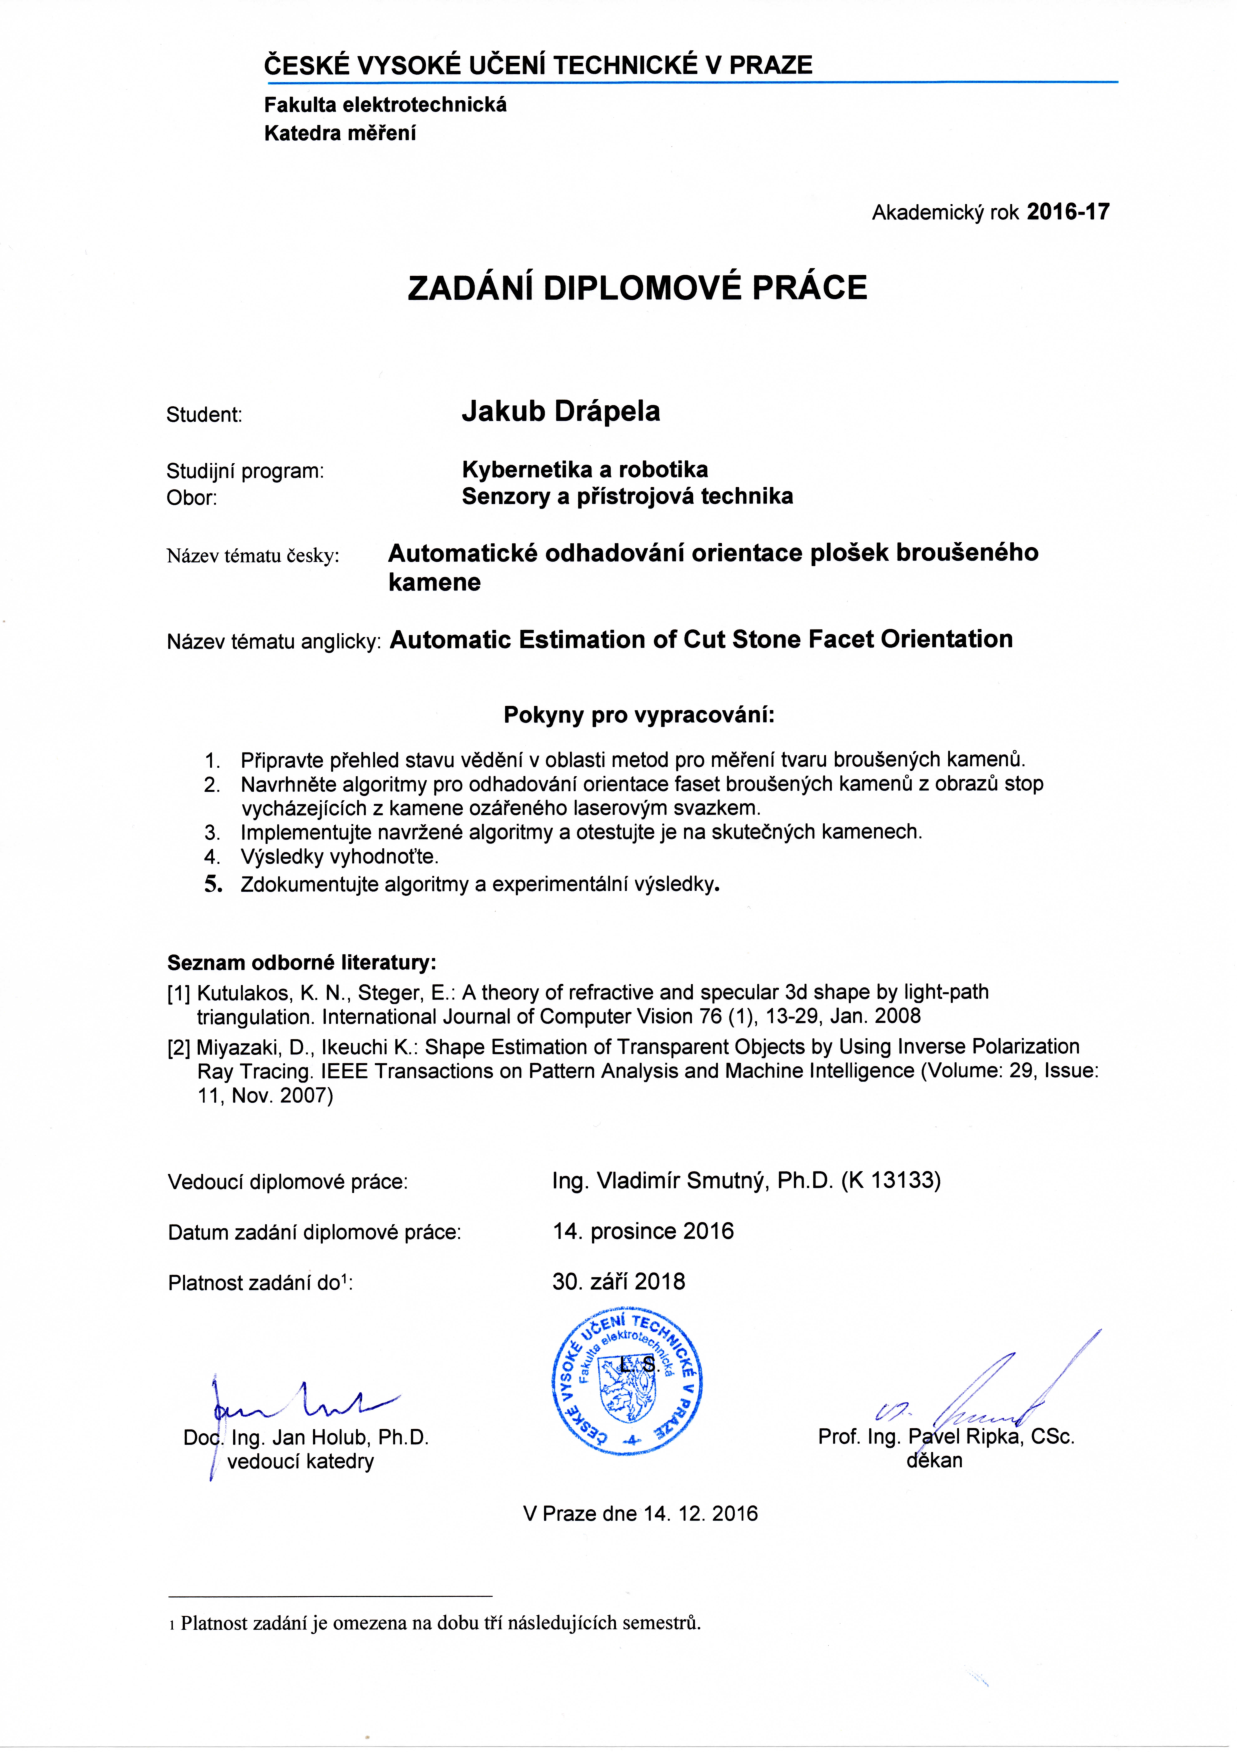
\includegraphics[width=\paperwidth,height=\paperheight]{zadani.pdf}
%\end{textblock*}
%\mbox{}
%\newpage
%\thispagestyle{empty}
%\begin{textblock*}{\paperwidth}(0mm,0mm)
%  \noindent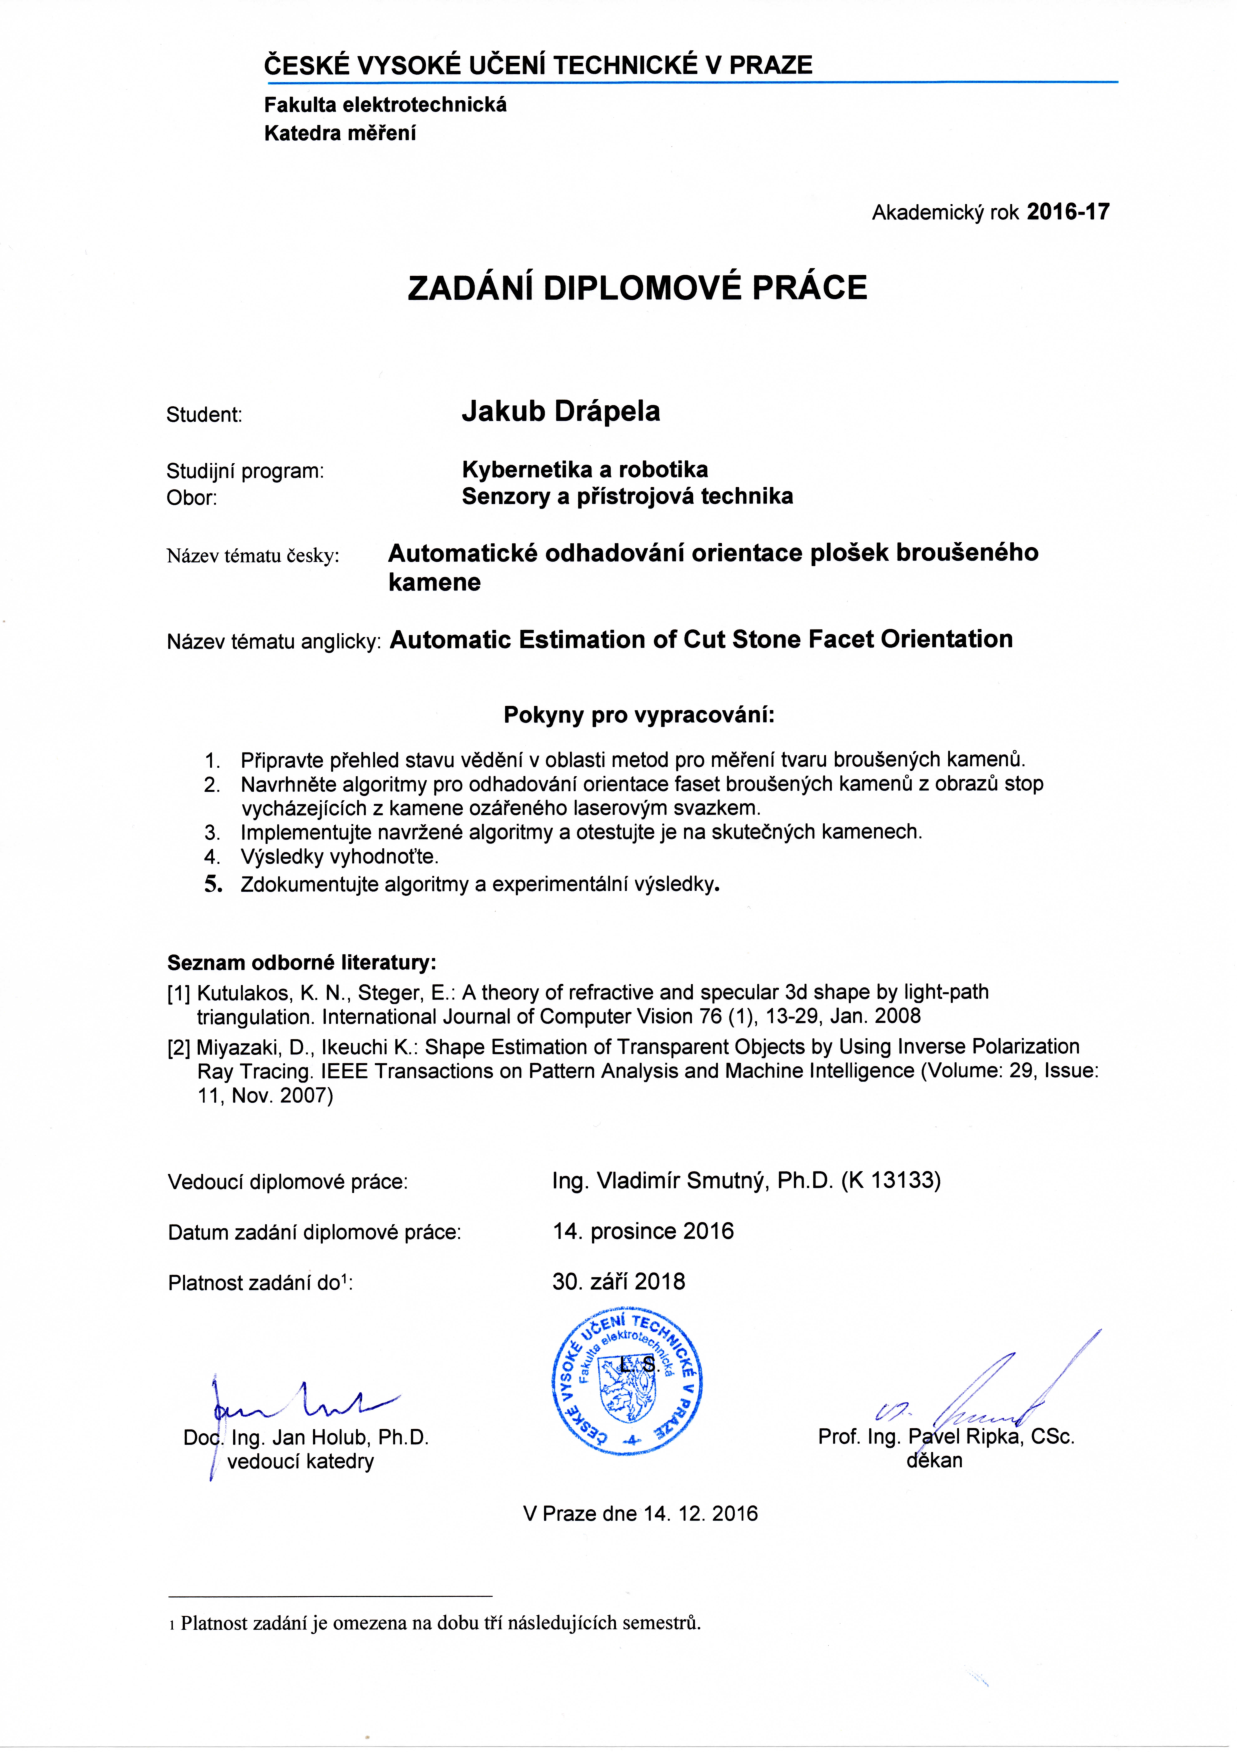
\includegraphics[width=\paperwidth,height=\paperheight]{zadani.pdf}
%\end{textblock*}
%\mbox{}
%\newpage
%\thispagestyle{empty}
%\begin{textblock*}{\paperwidth}(0mm,0mm)
% % \noindent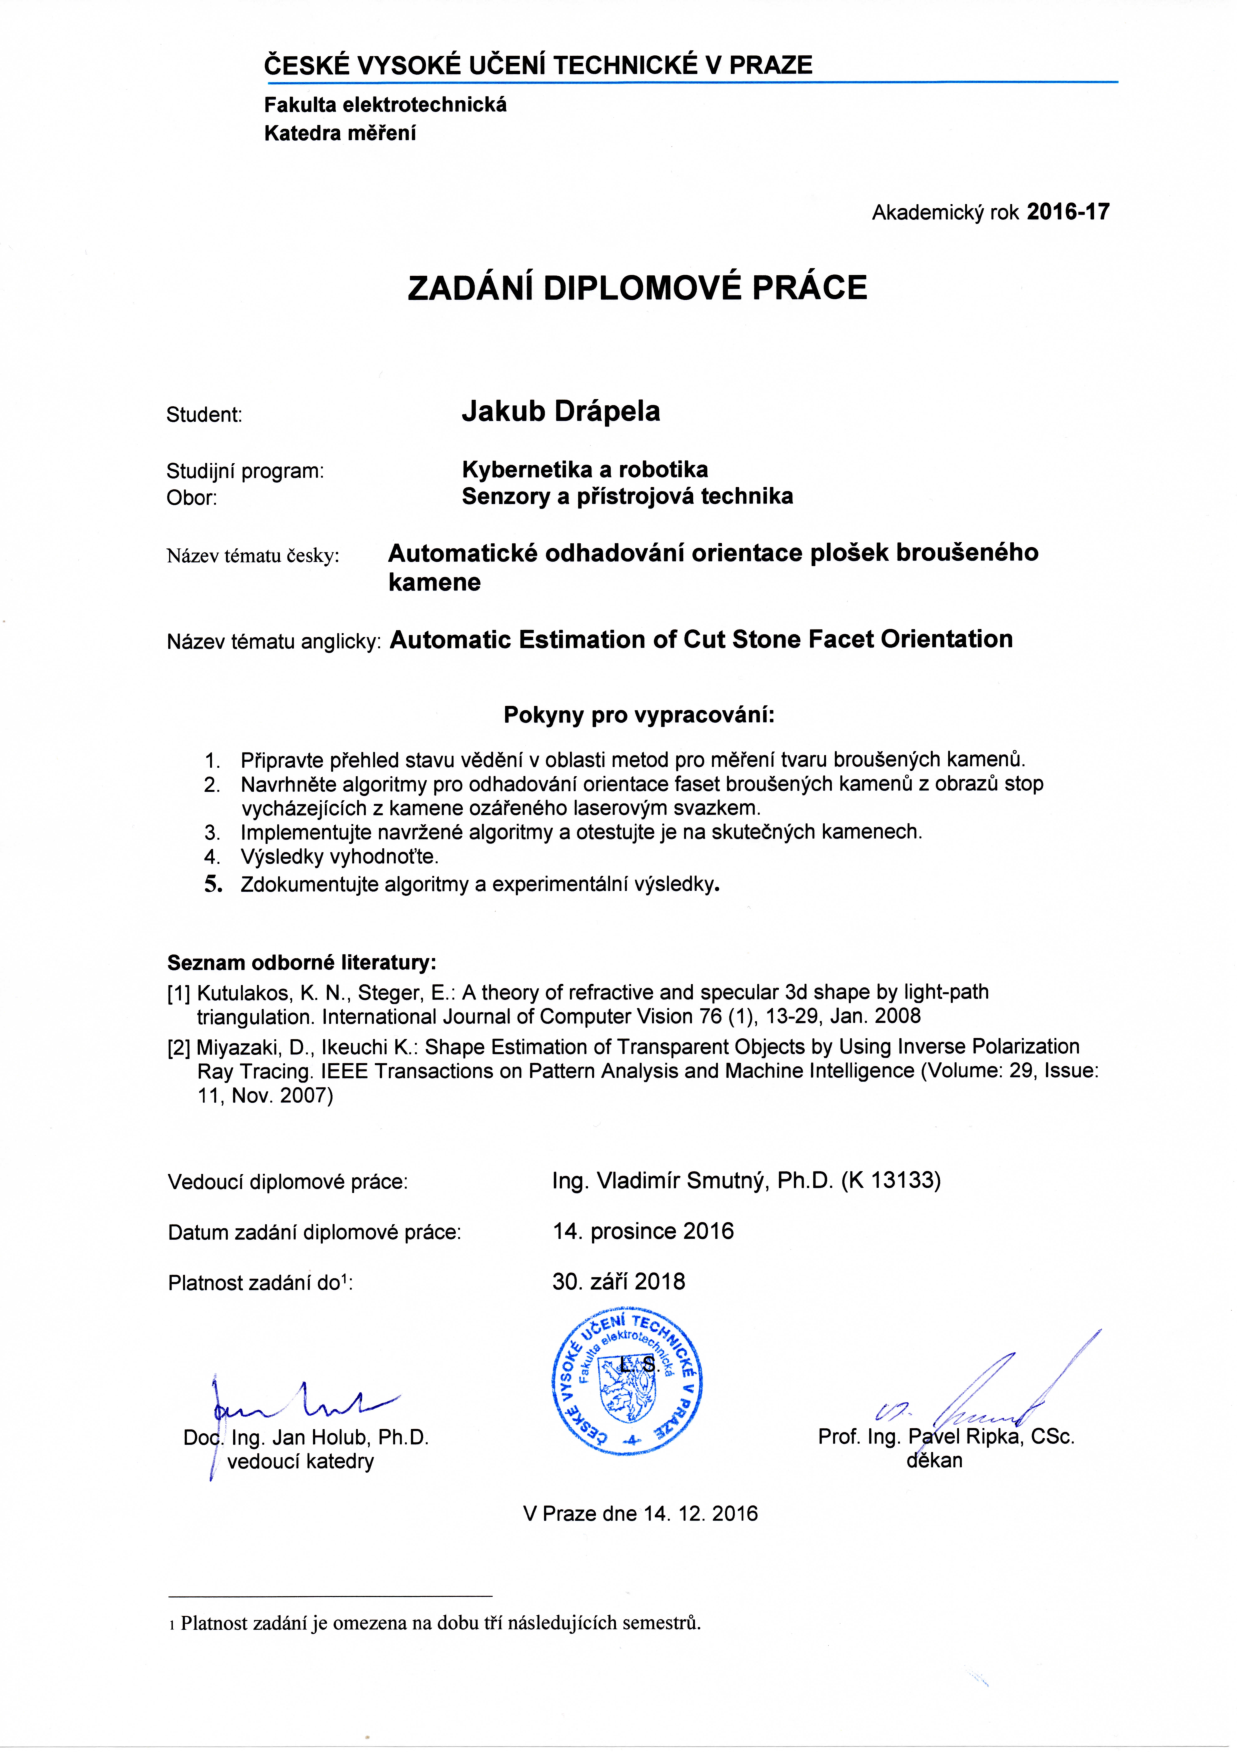
\includegraphics[width=\paperwidth,height=\paperheight]{zadani.pdf}
%\end{textblock*}
%\mbox{}
%\newpage


%\pagestyle{pagestyle_blue_rule}
%\newgeometry{ left=4.7cm,right=3.0cm,top=3cm,bottom=4cm, twoside=false}
%
%\pagenumbering{roman}
%%% prohlaseni,podekovani,abstrakt %%%%%%%%%%%%%%%%%%%%%%%
%	\newpage
%	\null \vfill{}
\section*{Prohlášení}
		
%I hereby declare that I have completed this thesis independently and that I have used only
%the sources (literature, software, etc.) listed in the enclosed bibliography.
%Prohlašuji, že jsem svou bakalářskou práci vypracoval samostatně a použil jsem pouze podklady (literaturu, projekty, SW %atd.) uvedené v přiloženém seznamu.

Prohlašuji, že jsem předloženou práci vypracoval samostatně a že jsem uvedl veškeré použité informační zdroje v souladu s Metodickým pokynem o dodržování etických principů při přípravě vysokoškolských závěrečných prací.\\[0.5cm]

V Praze dne $\dots\dots\dots\dots \dots\dots$ \hspace{2.5cm}$ \dots\dots\dots\dots \dots\dots\dots\dots$

\hspace{8.6cm}Podpis autora práce
\begin{figure}[!h]
	\begin{flushright}
		%\includegraphics[width=7cm]{fig/podpis.jpg}
	\end{flushright}
\end{figure}
\\
%	\newpage
%	\null 
\section*{Poděkování}

Zde bych chtěl poděkovat za podporu při tvorbě této bakalářské práce. Poděkování patří především mému vedoucímu Ing. Vladimíru Smutnému, Ph.D. za poskytnuté konzultace, vstřícnost, ochotu a trpělivost. 

Dále bych rád poděkovat rodině za podporu během studia. Nemalé díky patří také přátelům za silnou morální podporu a rady, které mi pomohly tuto práci realizovat.   

\vfill{}
%	\newpage
%	\section*{Abstrakt}
Tato práce se zabývá návrhem a kalibrací soustavy pro měření šíření laserového svazku šperkařskými kameny. Zkalibrovaná soustava bude použita k porovnání naměřených výsledků z měřeného kamene s jeho matematickým modelem. Porovnáním lze zjistit tvar kamene a kvalitu brusu, čehož se využívá např. pro určení ceny kamene nebo k seřizovaní brusných kotoučů při výrobě.   

Úkolem kalibrace navržené měřicí soustavy je nalezení správné transformace mezi pixely z pořízeného snímku a úhlem, pod kterým světelný paprsek opustil broušený šperk. Kalibrace probíhá postupně v několika krocích. Prvním krokem je nalezení projekční matice a radiálního zkreslení kamery. V dalším kroku s pomocí stereo-rekonstrukce hledáme parametry stínítka a nakonec optimalizujeme parametry laserového svazku. Pro optimalizaci použijeme nelineární metody minimalizace. 

\textbf{Klíčová slova:} kalibrace kamery, korespondence obrazů, triangulační metoda, optimalizace parametrů 

\section*{Abstract}
	This thesis describes the design and calibration of system for measuring the spread of the laser beam in the cut gemstone. Calibrated system will be used to compare results measured on the stone with its mathematical model. We can determine the shape and quality of the cut stone by comparing which is used e.g. to determine stone price or to adjust grinding wheel in the production.

The task of calibration is to find the correct transformation between the pixels in captured image and the direction of the light beam leaves the cut jewel. Calibration is carried out in several steps. The first step is to find the projection matrix and the radial distortion of the cameras. In the next step, we use stereo-reconstruction to find parameters of shade and then we optimize the parameters of the laser beam. We use nonlinear minimization methods to optimize.

\textbf{Keywords:} camera calibration, image correspondence, triangulation method, parameter optimization

%	\newpage
%%% obsah %%%%%%%%%%%%%%%%%%%%%%%%%%%%%%%%%%%%%%%%%%%%%%%%
%	\tableofcontents
%	\newpage
%%% seznam obrazku a tabulek %%%%%%%%%%%%%%%%%%%%%%%%%%%%%	
%	\listoffigures
%	\newpage
%	\listoftables
%%	\newpage
%%	\listoflistings
%\restoregeometry
%\clearpage
%
%%% stranka s naskenovanym zadanim prace %%%%%%%%%%%%%%%%%
%\thispagestyle{empty}
%\mbox{}
%\newpage

\pagestyle{pagestyle_text}
\pagenumbering{arabic}
%% VLASTNI PRACE %%%%%%%%%%%%%%%%%%%%%%%%%%%%%%%%%%%%%%%%
\newpage
\chapter{Úvod}

Drahé kameny jsou lidstvem od pradávna vyhledávány.
Jsou znakem krásy, bohatství a moci. Z počátku se kameny leštily do oblých tvarů a stávaly se součástí šperků.
S vývojem civilizace se začaly drahé kameny brousit, aby se zvýraznil lom světla a lesk minerálu. Broušením vznikaly rovinné fasety. Kombinací faset s definovanou velikostí a sklonem se vyvinuly standardní tvary jako brilliant, trilliant, rosette,baguette apod. Drahé a velmi cenné suroviny jako diamant se brousí pouze ručně. Méně významné kameny jsou převážně opracovávány automatickými stroji.  

Cenu broušených kamenů určují čtyři základní parametry. Mezi ně patří čistota, barva, hmotnost a kvalita brusu. 

Čistota určuje množství příměsí v materiálu kamene. Při tvorbě krystalu mohou dále vzniknout praskliny či vzduchové bubliny. 

Broušené kameny dělíme do široké řady odstínů. Barva kamene závisí jeho chemickém složení. Důležitá je v tomto ohledu jednotnost barev.

Hmotnost souvisí s velikostí kamene. U diamantů se hmotnost určuje v karátech  a je natolik důležitá, že se v některých případech volí kompromis mezi kvalitou brusu.

Brus je důležitá mechanická úprava kamene. Ideálně opracovaný kámen má dokonalý soulad mezi brilancí, ohněm a jiskřením. Mezi parametry hodnotící kvalitu brusu patří kvalita povrchového opracování faset. Fasety se brousí rovinnými brusnými kotouči. Broušením mohou vzniknout rýhy, škrábance, prohlubně, abraze na hranách (zbroušení přechodu mezi fasetami), povrchová oxidace a nové fasety. Kámen je třeba brousit s vysokou přesností. Každá odchylka velikosti a úhlu fasety od ideálního tvaru zhorší optické vlastnosti kamene. Orientace faset je proto důležitým parametrem pro zhodnocení kvality brusu.

Jedním z nástrojů ke zkoumání optických vlastností broušeného kamene je nasvícení jeho povrchu světelným svazkem. Na fasetách broušeného kamene dochází ve zjednodušeném případě k odrazu a lomu světelného svazku. Z toho důvodu se dopadající svazek roztříští na řadu světelných svazků různých tvarů. Svazky jsou definovány směrem šíření, zářivým tokem a elektromagnetickými parametry. 

Barva, čistota a kvalita brusu mají za následek změnu geometrie svazků. Ta je jednoznačným popisem broušeného kamene. Hodnocením vystupujících svazků můžeme určit parametry kamene. 

Tato práce navazuje na dlouhodobý výzkum v Centru strojového vnímání na katedře kybernetiky Elektrotechnické fakulty ČVUT. 


První práce, která se zabývá průchodem nerozbíhajícího se svazku konvexním tělesem je software LADOK \cite{Pohl2002} od Petra Pohla.  

Práce využívá software LADOK \cite{Pohl2002} od Petra Pohla. Simulační program LADOK zavádí pro broušený kámen geometrický model ve formě konvexního mnohostěnu s rovnými ploškami, fasetami. Na povrch kamene dopadá svazek nerozbíhajících se paprsků světla z definovaného směru. LADOK řeší odrazy, lomy a dělení svazků na povrchu kamene. Svazky po opuštění kamene mají definovaný směr, zářivý tok, plochu a tvar. Tento software rozšířil Igor Bodlák \cite{bodlakLADOK} o výpočet elekromagnetické vlastnosti svazků. Matematický model kamene obohatil Martin Straka \cite{strakaLADOK}. Přechody mezi fasetami modeloval jako posloupnost většího počtu menších faset s nenulovým poloměrem křivosti. 

LADOK je matematickým řešením experimentu na obr. \ref{fig:basicMeasure}. Zdrojem světla je laser. Laserový svazek dopadá na broušený kámen, kde se roztříští na mnoho menších svazků. Ty jsou po opuštění kamene zachyceny na stínítku. Stínítko snímáme kamerou a získáváme obraz svazků na stínítku.  


\begin{figure}[h!]
\begin{center}
\scalebox{0.5}{ \input{xfig/stinitko.pstex_t}}
\end{center}
\caption{Nákres principu experimentu. Laser produkuje svazek světla, který dopadá na celou plochu kamene. V kameni se svazek roztříští na mnoho svazků. Svazky vystupující z kamene v horní polorovině dopadnou na stínítko. Stínítko snímá kamera. Převzato z \cite{Drapela}.}
\label{fig:basicMeasure}
\end{figure}


Experimentální soustavu máme sestavenou a zkalibrovanou \cite{Drapela}. Známe transformaci mezi obrazem svazku na stínítku a směrem, ve kterém opouští kámen. 

O možnost porovnání dat reálného experimentu s výsledky počítačové simulace se postaral Igor Bodlák \cite{Bodlak2005}. Navrhl optimalizaci kritéria hodnotící rozdíl vzdálenosti stop z experimentu a odrazů stop simulace na stínítku. Optimalizovaly se parametry faset kamene a kámen se tak deformoval, aby se dosáhlo co nejlepší shody v zadaném kritériu. Software pro řešení inverzní úlohy nazval zkratkou LAM. 

LAM byl použitelný pouze pro broušený kámen čtvercového tvaru. Z důvodu složitosti přiřazení stop z experimentu k obrazům simulovaných svazků při osvětlení celého kamene zaměřil vstupní laserový svazek pouze do určitých míst kamene. Tím vzniklo redukované množství svazků a korespondence se simulovanými svazky se výrazně zjednodušila. Nevýhodou tohoto přístupu jsou rozměry kamene, které musí být několikanásobně větší než průměr laserového svazku. Metoda je prakticky nepoužitelná pro kameny o rozměrech v jednotkách milimetru. 

	V této práci osvítíme laserovým svazkem celý kámen. Zaměříme se na kameny šatonové růže s plochým spodkem a 12-ti bočními fasetami. Tyto kameny se ve zkratce nazývají \textit{viva12}. Rozměry kamenů budou v řádech milimetrů. 
	
	K robustní detekci obrazu svazků použijeme MSER detektor \cite{Matas}. Z výsledku detekce určíme parametry stop. Sestavíme program, pomocí kterého bude možno manuálně párovat obrazy svazků broušeného kamene se simulovanými stopami.
 Optimalizací z LAMu získáme náklony faset. Parametry svazků prozkoumáme pomocí určených experimentů. Navrhneme algoritmus pro \textit{vivu12}, který určí automaticky orientaci faset kamene. Výstupem programu budou odchylky úhlů faset kamene od jejich ideální pozice.


















\chapter{Fyzikální model}

\section{Model kamene}
Broušený kámen je modelován jako konvexní mnohostěn \cite{Pohl2002}. Brusné kotouče považujeme za dokonale rovinné. Uchycení kamene při broušení zjednodušíme na absolutně tuhé bez známek pružnosti či ohybu. Fasety potom můžeme modelovat jako rovné plochy. Orientace a umístění fasety získáme z výkresu nebo předchozího měření. 

Přechody mezi fasetami jsou v ideálním případě ostré hrany. Z důvodu abraze hran v procesu výroby kamene jsou hrany obroušeny do oblého tvaru. K přiblížení modelu reálnému obroušení hran aproximujeme hranu množstvím rovinných faset se vzájemnou polohou odpovídající poloměru křivosti hrany.  
  
\begin{figure}[htps]
\centering
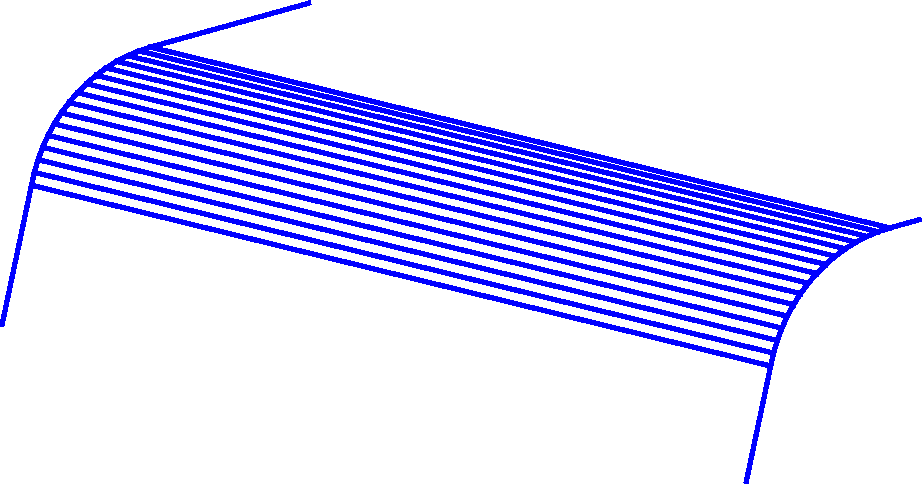
\includegraphics[width=0.6\linewidth]{edge_ex.pdf}
\caption{Detail aproximace přechodu mezi fasetami.}
\label{fig: edge}
\end{figure}  

\section{Model svazku}
Svazek světla v LADOKU reprezentuje nerozbíhající se konvexní hranol. Vlivem odrazu a lomu se konvexní tvar zachová. Fasety jsou také konvexní, proto se konvexita zachová i při štěpení svazku. Po opuštění kamene jsou svazky definovány zářivým tokem, plochou a směrem, které lze vyjádřit pomocí azimutu a elevace. Stokesovy koeficienty definují elektromagnetické vlastnosti svazku. 

Zaznamenána je celá cesta svazku. V každém bodě trasy máme k dispozici posloupnost směrů a tvarů svazku vyjádřeném pomocí polygonu. 

Model nepostihuje situace, při kterých nastává rozbíhavost světla.
\begin{itemize}
\item Pokud jsou v materiálu přítomné nečistoty, praskliny, vzduchové bubliny apod., světelný svazek se rozptýlí.
\item  Rozptyl světelných svazků vzniká vlivem nedokonalého vyleštění faset a to jak při lomu tak při odrazu.
\item Vlivem oxidace při leštění mohou vzniknout místa s jiným indexem lomu než je index lomu materiálu. Podobný případ nastane pokud má kámen nejednotný odstín.

\item Přítomnost hran v kameni způsobí ohyb světla (difrakci).
\end{itemize}

Část zářivého toku svazku může být pohlcena a přeměněna na teplo.

\section{Model stínítka}
\label{sec:stinitko}
Po dopadu laserového svazku na stínítko se záření difuzně odrazí. Odrazivé vlastnosti materiálu závisí na úhlu odpadajícího světla a lze je matematicky popsat pomocí modelu zvaného BRDF (Bidirectional reflectance distribution function). Odražené světlo zvýší intenzitu světla nejen v místě dopadu světelného svazku, ale i v jeho okolí.

Odražené světlo zároveň putuje do kamene a od něj zpět na stínítko. 

%%tohle bych zařadil na později
%Laserové stopy chceme detekovat v černobílém HDR snímku půlkulového stínítka, na které dopadá část laserových svazků vystupujících z nasvíceného kamene. Snímek ze zatížen radiálním zkreslením, které je způsobeno vlastností optické soustavy objektivu. Radiální zkreslení bylo určeno v předchozí bakalářské práci \cite{Drapela}. Snímek lze pomocí transformace z \cite{Drapela} zkreslení zbavit. Z \cite{Drapela} navíc známe transformaci mezi pozicí bodu v nezkresleného snímku a odpovídajícím parametrům azimutu a elevace.



V ideálním případě lze ve snímaném obraze pozorovat pouze dopady světelných svazků, které vznikly kombinací odrazů a lomů zdrojového svazku od faset broušeného kamene. U reálného kamene ovšem v obraze pozorujeme tenké slábnoucí přímky vycházející ze stopy světelného svazku, ocásky. Tyto ocásky vznikají díky lomu/odrazu světelného svazku od neostrých hran broušeného kamene.

\begin{figure}[h!]
\begin{center}
\scalebox{.9}{ \input{xfig/tails.pstex_t}}
\end{center}
\caption{Příklad snímaného obrazu s vyznačením obrazů svazků a ocásků.}
\label{fig:tail_ex1}
\end{figure}


Vnik ocásků si ukážeme při lomu světla na oblé hraně kamene. Situaci budeme uvažovat v 2D prostoru, kde platí obecně stejné principy jako ve 3D. Světlo nahradíme paprsky světla se směrem šíření $\vec{v_i}$. 

Zvolíme si dvě fasety, které svírají úhel \SI{45}{\celsius}. Ostrý přechod aproximujeme. Vznikne posloupnost úseček, které propojují fasety. Každé úsečce přiřadíme normálový vektor $\vec{n}$.  

\begin{figure}[htp]
\centering
\begin{minipage}[c]{0.48\textwidth}
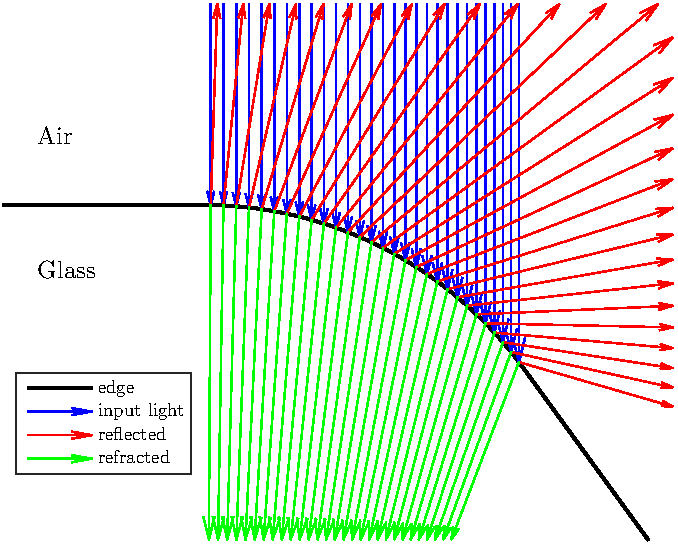
\includegraphics[width=\textwidth]{edgeIn.pdf}
\end{minipage}
\begin{minipage}[c]{0.48\textwidth}
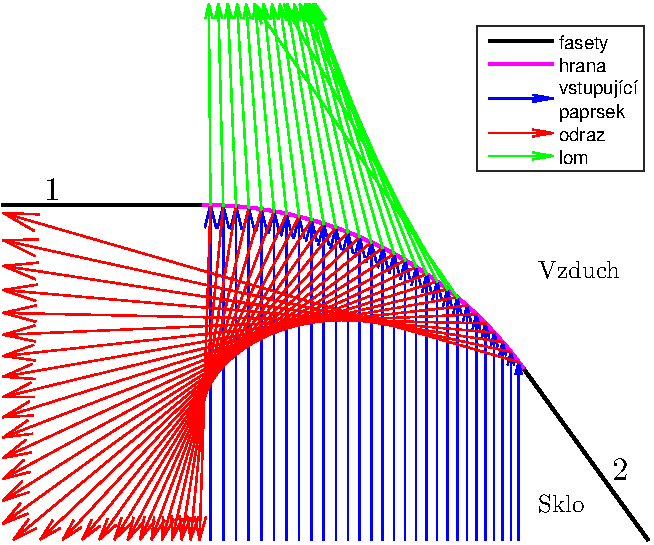
\includegraphics[width=\textwidth]{edgeOut.pdf}
\end{minipage}
\caption{Dopad světelných paprsků na hranu. Paprsky se lomí vlevo ze vzduchu do skla a vpravo ze skla do vzduchu. Situace pro index lomu vzduchu $n_a = 1$ a index lomu skla $n_g = 1.5$.}
\label{fig:edgeIn}
\end{figure}
Z Fresnelových rovnic víme, že dochází nejen k lomu světla, ale část světla000 se odrazí. Poměr intenzity odraženého a lomeného světla závisí na polarizaci světla a dopadajícím úhlu. V této ukázce uvažujeme nepolarizované světlo. 

Aplikací Snellova zákonu a zákonu odrazu na $\vec{n}$ a $\vec{v_i}$ vypočítáme směr lomu a odrazu světelných paprsků.

Na obr. \ref{fig:edgeIn} dopadají paprsky světla ze vzduchu na sklo i ze skla do vzduchu. V odou případech se odražené i lomené paprsky projeví jako ocásky.

Pokusíme se prozkoumat intenzitu ocásků $I$ v závislosti na vystupujícím úhlu, elevaci $\varepsilon$. 
Pro jednotlivou elevaci určíme intenzitu relevantně ke vstupující intenzitě jako 
\begin{equation}
 I_\varepsilon  = \frac{\rho_{{max}}}{\rho_\varepsilon}\cdot R
\end{equation}
pro odražené paprsky a 
\begin{equation}
 I_\varepsilon  = \frac{\rho_{\varepsilon_{max}}}{\rho_\varepsilon}\cdot (1-R)
\end{equation}
pro lomené paprsky, kde  

	\begin{tabular}{l l}
	$\rho_{\varepsilon}$ & 	- hustota paprsků pro danou elevaci $\varepsilon\,$,\\
	$\rho_{{max}}$  	&	- maximální hustota paprsků ve všech elevacích,\\
	$R_\varepsilon$		&	- odrazivost z Fresnelových rovnic pro $\varepsilon\,$.	 \\
	
	\end{tabular}

Závislost $I(\varepsilon)$ je označená jako \textit{Reflection coefficient} resp. \textit{Refraction coefficient} na obrázcích \ref{fig:edgeInGraf} a \ref{fig:edgeOutGraf}.


\begin{figure}[htps]
\centering
\begin{minipage}[c]{0.48\textwidth}
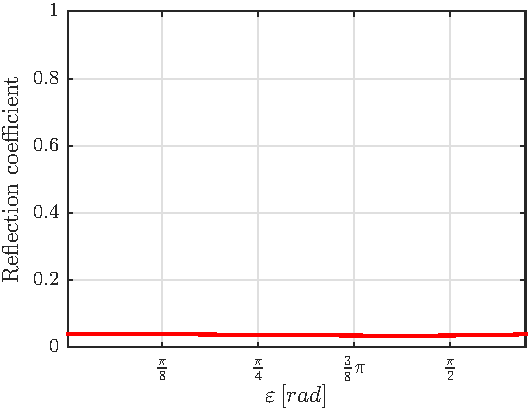
\includegraphics[width=\textwidth]{edgeIn_reflection.pdf}
\end{minipage}
\begin{minipage}[c]{0.48\textwidth}
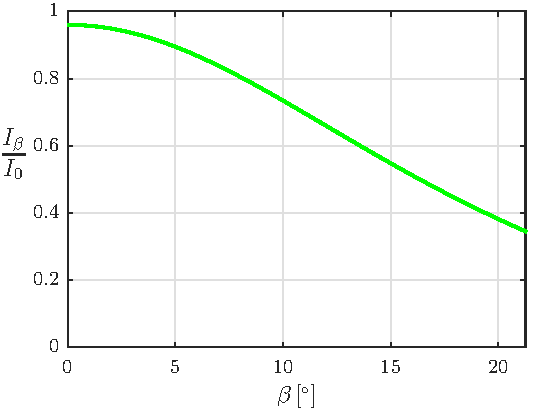
\includegraphics[width=\textwidth]{edgeIn_refraction.pdf}
\end{minipage}
\caption{\textit{Reflection coefficient} resp. \textit{Refraction coefficient} v případě když se lomí světlo ze vzduchu do skla (obr. \ref{fig:edgeIn}).}
\label{fig:edgeInGraf}
\end{figure}

\begin{figure}[htps]
\centering
\begin{minipage}[c]{0.48\textwidth}
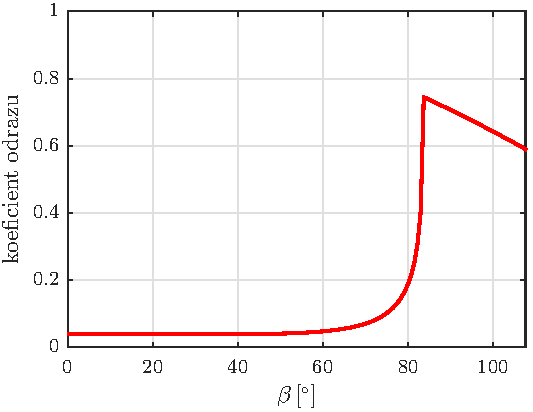
\includegraphics[width=\textwidth]{edgeOut_reflection.pdf}
\end{minipage}
\begin{minipage}[c]{0.48\textwidth}
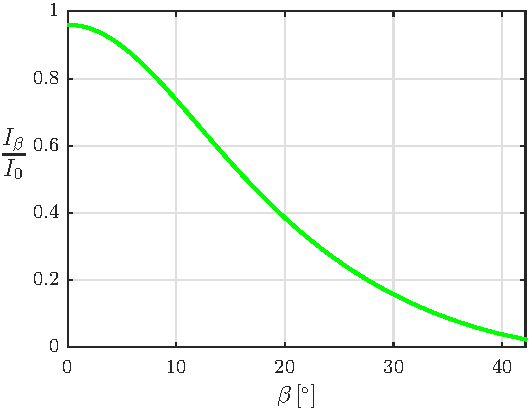
\includegraphics[width=\textwidth]{edgeOut_refraction.pdf}
\end{minipage}
\caption{\textit{Reflection coefficient} resp. \textit{Refraction coefficient} v případě když se lomí světlo ze skla do vzduchu (obr. \ref{fig:edgeIn}).}
\label{fig:edgeOutGraf}
\end{figure}

Z grafů \ref{fig:edgeInGraf} a \ref{fig:edgeOutGraf} je patrné, že ocásky budeme pozorovat různě dlouhé a z vysokou variabilitou z hlediska intenzity. 
	  

 Intenzita a délka ocásku je ovlivněna i dalšími faktory, jako je např. délka hrany, čistota hrany, drsnost povrchu atd. Všechny faktory, které ovlivňují intenzitu ocásku prozatím nejsme schopni v programu LADOK zahrnout do matematického modelu, proto pro prování svazků bude užitečná především informace o směru ocásku. 
 
 

\section{Model obrazu}

Obraz snímaný kamerou je zatížen radiálním zkreslením. Zkreslení odstraníme pomocí kalibrace kamery \cite{Drapela}. 


\section{Model Kamery}
\label{sec:poisson}
 Použitý CCD snímač má $2050^2$ pixelů. Každému pixelu odpovídá jeden samostatný snímač, který funguje na principu počítání přicházejících fotonů po dobu expozice. Počet přicházejících fotonů v daném časovém intervalu se řídí Poissonovým rozdělením. Pravděpodobnost, že napočítáme $n$ fotonů je 
 
 \begin{equation}
    P(\mathrm{X} = n)=\frac{\lambda ^{n}\,\mathrm{e}^{-\lambda}}{n!}\,,
 \end{equation}
 kde $\lambda$ je střední hodnota a $\mathrm{X}$ náhodná veličina.













\part{Detekce světelných stop v obraze}
\label{sec:detection}

\section{Jevy v obraze}
Pro analýzu vlastností broušeného kamene je důležité detekovat světelné stopy vzniklé dopadem laserových svazků na stínítko. Zároveň je třeba určit parametry stop, které se budou porovnávat s parametry svazků matematického modelu kamene. 

Intenzitu pixelu $I$ můžeme vyjádřit pomocí Poissonova rozdělení jako 
\begin{equation}
	I = \mathrm{Pois}\left(I_{s}+I_{p}+I_{o}\right)\,,
	\label{eq:intensitu_sum}
\end{equation}
 kde $I_{s}$ reprezentuje příspěvek světelného svazku, $I_{p}$ intenzitu pozadí, $I_{o}$ intenzitu světelných ocásků. Jedním z úkolů detektoru je oddělit pozadí od zbývajících složek intenzit. %Po odečtení pozadí získáme obrazy laserových svazků.   
 
Jednoduchým postupem pro určení intenzity pozadí by bylo prahování obrazu nad konstantní úrovní. V našem obraze však typicky konstantní není (kapitola \ref{sec:stinitko}). 

\begin{figure}[h!]
\centering
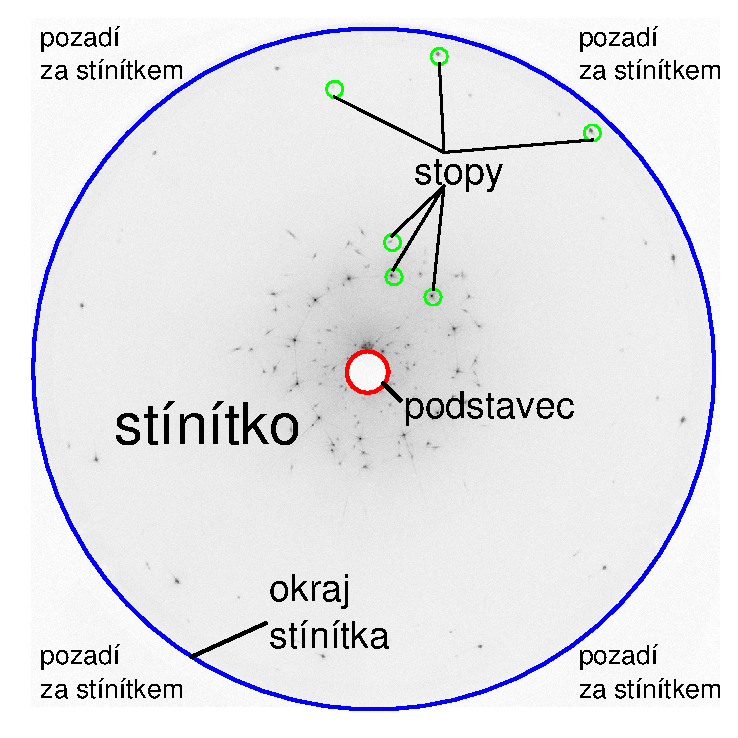
\includegraphics[width = 0.5\textwidth]{stinitkoSnimek.eps}
\caption[Popis objektů v obraze.]{Popis objektů v obraze.}
\label{fig: podstavec}
\end{figure}


Rozdílné pozadí se může také vytvořit odrazem zdrojového svazku od jiných předmětů, než broušeného kamene. Hlavním příspěvkem je v tomto případě odraz od podstavce, na který pokládáme broušený kámen (obr. \ref{fig: podstavec}).

\begin{figure}[h!]
\centering
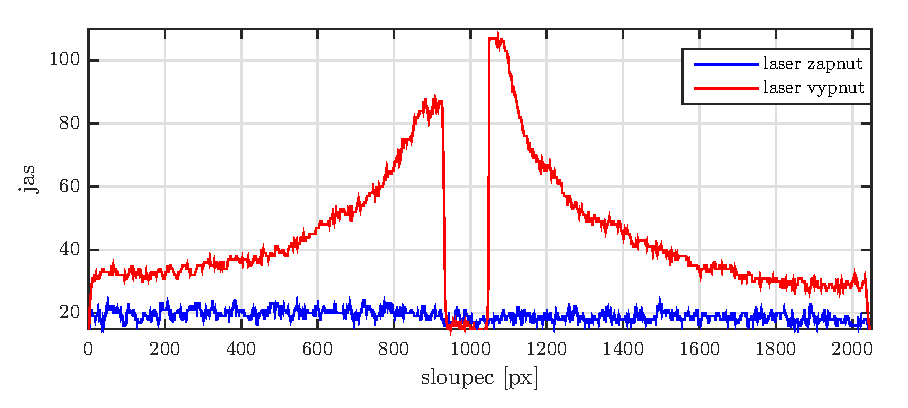
\includegraphics[width = 0.6\textwidth]{podstavec.eps}
\caption[Vliv odrazu od podstavce na pozadí snímku.]{Jasové úrovně ve vybraném řádku obrazu. Řádek protíná obraz podstavce. V případě červené charakteristiky dopadá na podstavec laserový svazek, rozptyluje se a dopadá na stínítko. Modrou charakteristiku pozorujeme, pokud je laser vypnutý.}
\label{fig: podstavec}
\end{figure}

Hodnotu pozadí potřebujeme znát, abychom ze snímku mohli vypočítat světelný tok pro jednotlivé dopadající laserové svazky. Určení intensity pozadí v každém pixelu komplikuje obraz podstavce na kámen a okolí stínítka. Zde je intenzita světla podstatně nižší, než na povrchu stínítka. Vysoká změna jasu v obraze komplikuje určení pozadí.  

V okolí stínítka můžeme detekovat falešné svazky, které je třeba odstranit. 

Světelné stopy se mohou překrývat. Pro odlišení příspěvků jednotlivých svazků je třeba obraz prahovat v několika úrovních jasu.

V místě, kde je vysoká koncentrace svazků mohou svazky dopadnout tak blízko sebe, že splynou v jednu stopu (obr. \ref{Splynuti}).  

\begin{figure}[h!]
    \centering
    \begin{minipage}[c]{0.48\textwidth}
        \centering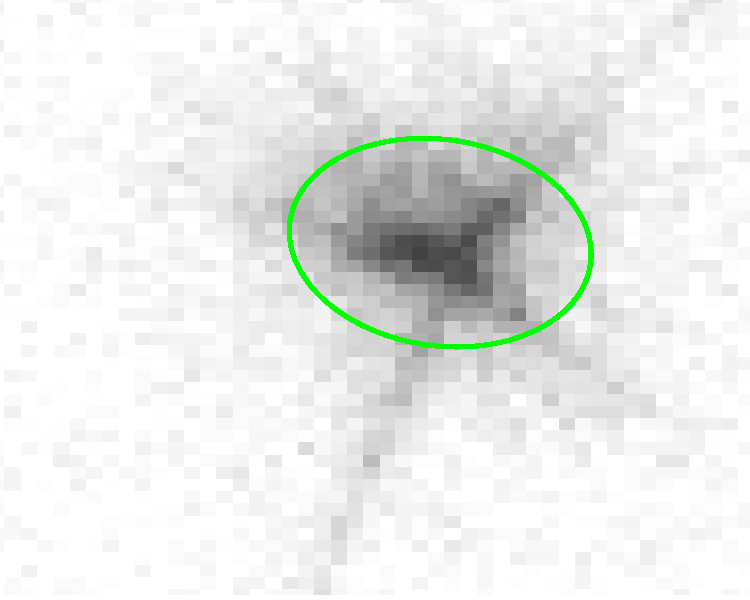
\includegraphics[width=.5\textwidth]{pf_near.pdf}
    \end{minipage}
    \begin{minipage}[c]{0.48\textwidth}
        \centering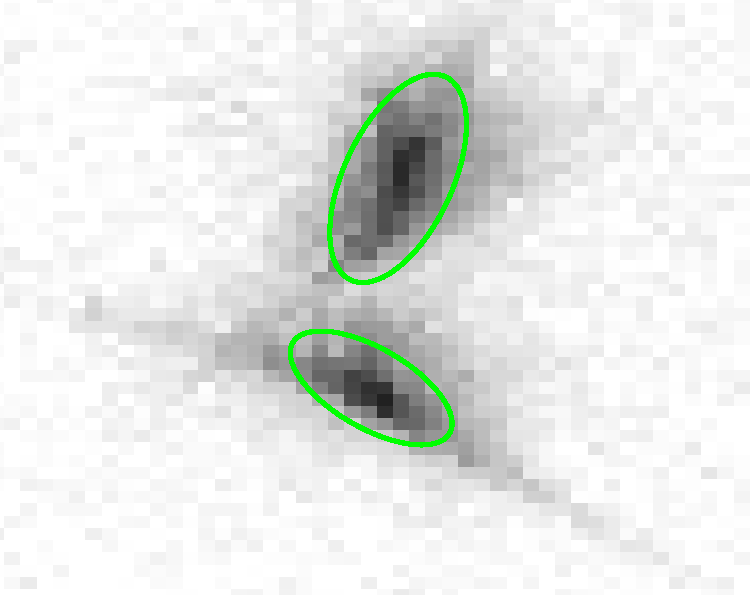
\includegraphics[width=.5\textwidth]{pf_near2.pdf}
    \end{minipage}
    \\
        \caption[Slynutí dvou různých svazků.]{Ilustrace slynutí dvou různých svazků. V pravém i levém snímku se nachází typově stejné laserové svazky. Na levém obrázku dopadly na stínítko příliš blízko sebe. V tomto případě nejsme schopni rozlišit příspěvek obou svazků a detekujeme pouze jednu stopu.}
        \label{Splynuti}
\end{figure}

Obraz je třeba filtrovat. Filtrováním snížíme šum v odraze, ale zároveň zmenšíme kontrast mezi stopami. 

Ne všechny svazky vystupující z kamene je možné detekovat. Svazky s vícenásobným odrazem postupně ztrácí zářivý tok. Po dopadu na stínítko mohou být nerozlišitelné od šumu a jejich detekce je prakticky nemožná. Pro stopy s nízkým jasem bude detekce často selhávat.

\begin{figure}[h!]
    \centering
    \begin{minipage}[c]{0.48\textwidth}
        \centering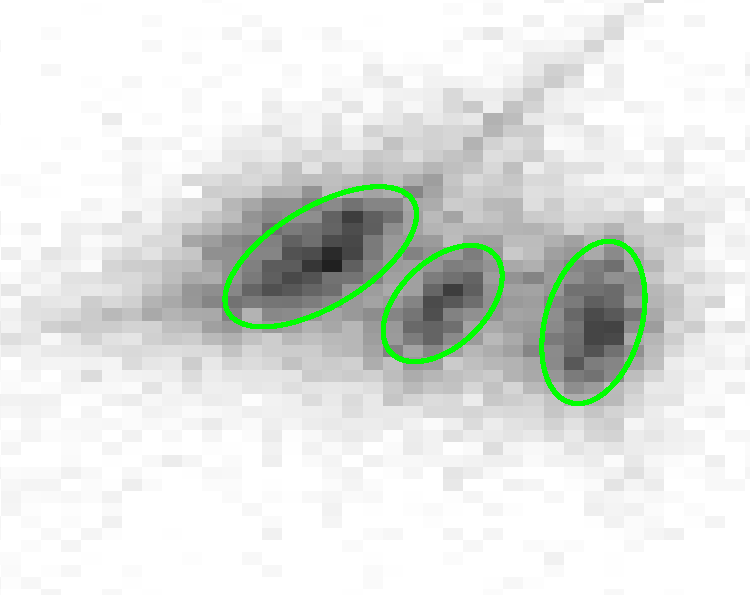
\includegraphics[width=.75\textwidth,height = 4.5 cm]{pf_punch2.pdf}
    \end{minipage}
    \begin{minipage}[c]{0.48\textwidth}
        \centering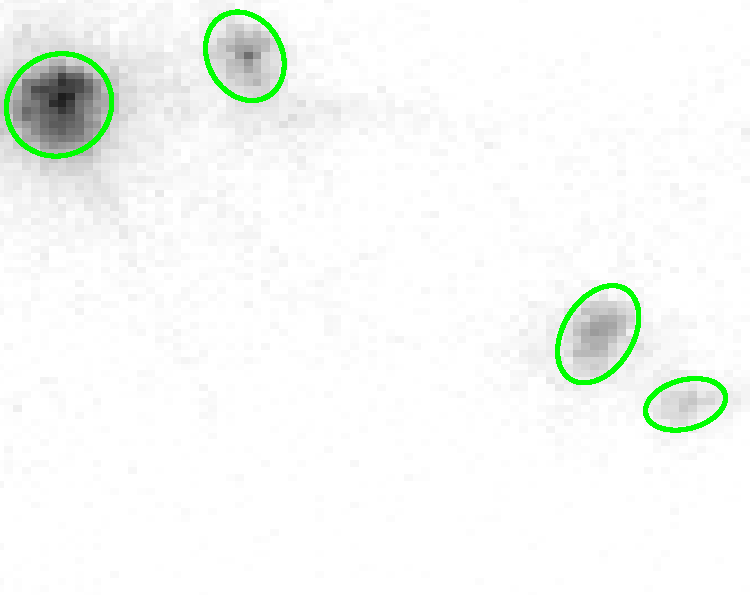
\includegraphics[width=.75\textwidth,height = 4.5 cm]{p_deff2.pdf}
    \end{minipage}
    \\
        \caption[Problémové detekce.]{Problémové detekce. Nalevo jsou laserové stopy blízko u sebe. Stopy je nutné od sebe oddělit. Na levém snímku jsou znázorněny výrazné rozdíly mezi velikostí a intenzitou stop. Je nutné použít víceúrovňový detektor. }
        \label{fig:Detekce}
\end{figure}

\newcommand\x{4}
\newcommand\xx{0,155}

\begin{figure}[h!]
    \centering
    \begin{minipage}[c]{0.163\textwidth}
        \centering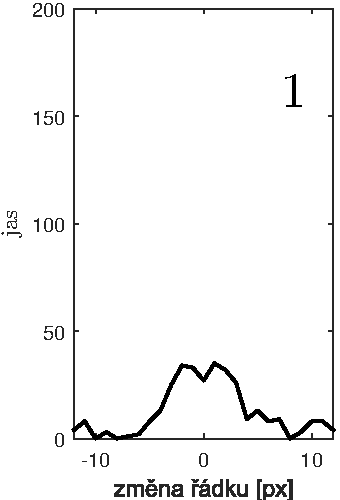
\includegraphics[height = \x cm,width = \textwidth ]{cut_1.pdf}
    \end{minipage}
    \begin{minipage}[c]{\xx \textwidth}
        \centering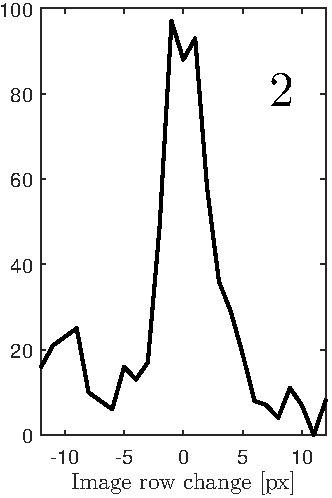
\includegraphics[height = \x cm,width = \textwidth]{cut_2.pdf}
    \end{minipage}
    \begin{minipage}[c]{\xx \textwidth}
        \centering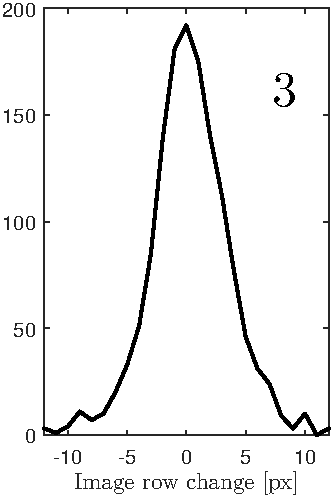
\includegraphics[height = \x cm,width = \textwidth]{cut_3.pdf}
    \end{minipage}
    \begin{minipage}[c]{\xx \textwidth}
        \centering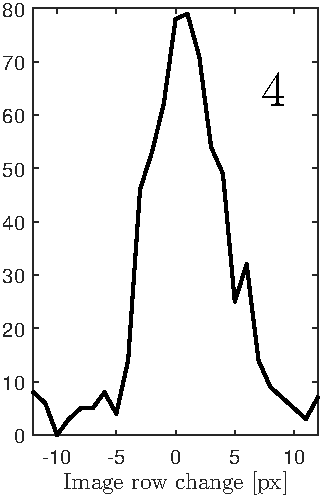
\includegraphics[height = \x cm,width = \textwidth]{cut_4.pdf}
    \end{minipage}
    \begin{minipage}[c]{\xx \textwidth}
        \centering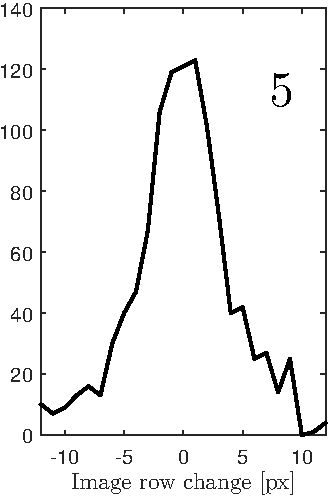
\includegraphics[height = \x cm,width = \textwidth]{cut_5.pdf}
    \end{minipage}
    \begin{minipage}[c]{\xx \textwidth}
        \centering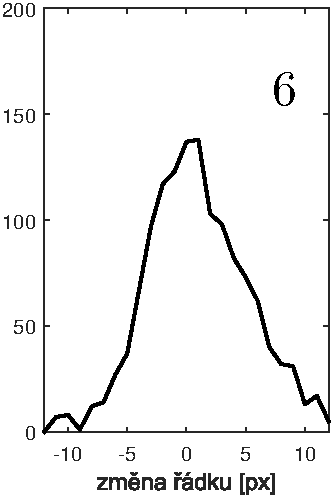
\includegraphics[height = \x cm,width = \textwidth]{cut_6.pdf}
    \end{minipage}
    \\
        \caption[Jasové řezy.]{Jasové řezy ve totožném sloupci obrazu. Řez protíná pixel s maximální hodnotou jasu ve stopě. Číslování řezů odpovídá indexům stop na obr. \ref{fig:Detekce}.}
        \label{fig:rezy}
\end{figure}


\section{Předchozí práce}

V předchozí práci \cite{Drapela} jsme neměli možnost detekovat stopy s nízkým jasem. Překrývající se svazky bylo nemožné oddělit.  

Bohatší pojetí problému se objevilo v Bodlákově práci \cite{Bodlak2005}. Snímek se prahoval více než jedním prahem. Z oblastí nad prahem se sestavila stromová struktura. Světelné stopy se určily jako listy stromu s dostatečnou významností. Tento přístup je však pro svou výpočetní náročnost nepoužitelný pro snímky s rozlišením 2050$\times$2050, které máme k dispozici. 

Naše úloha detekce je velmi podobná detekci hvězd a galaxií v astronomických snímcích. V oblasti astronomie se hojně používá program s názvem Source Extractor \cite{SEXarticle}. Tento program má za sebou dlouholetý vývoj, je optimalizován z hlediska rychlosti a odzkoušený širokou veřejností. Tento software lze po naladění parametrů použít i pro náš případ. Nevýhodou však je, že nelze spustit v operačním systému Windows, který využíváme.  

Po testu různých detektorů jsme se rozhodli pro detekci laserových stop v obraze využít relativně nový přístup uveden J. Matasem et al. \cite{Matas} v roce 2002 - MSER detektor. 




\section{MSER (maximal stable extremal region) detektor}

MSER detektor hledá v obraze maximálně stabilní extrémní oblasti. Původně byl využit pro robustní nalezení korespondencí mezi dvěma snímky stejného objetu pořízených z různého místa a v současné době se používá v mnoha oblastech počítačového vidění.  

Princip spočívá v několikaúrovňovému prahování obrazu podle intenzity a nalezení spojitých oblastí, které jsou nad či pod prahovou hodnotou. Mezi úrovněmi jsou nalezeny korespondující oblasti a za MSER oblasti jsou označeny ty, jejichž velikost z předchozí úrovně se se zvyšující úrovní příliš nezměnila. 

Výhodou MSER detektoru je invariance vůči afinní transformaci intenzity a vůči změně měřítka, což umožňuje současnou detekci malých a velkých oblastí s různou intenzitou. Podle studie \cite{Comparison}, která porovnává MSER detektor s ostatními typy detektorů významných oblastí, dosáhl MSER detektor skvělých výsledků v detekci oblastí s vysokou hustotu a variabilní změnou velikosti. MSER detektor se tedy zdá být vhodným kandidátem pro detekci laserových stop v obraze.

\section{Implementace}

\subsection{Filtrace}
   Nejprve se pokusíme minimalizovat Poissonův šum v obraze. Šum redukujeme konvolucí s maskou, která se skládá z prvků odpovídajících Gaussově funkci. Parametry filtru: velikost masky - \SI{3}{\px}, směrodatná odchylka $\sigma = $ \SI{0.7}{\px}.

\subsection{Detekce} 
   %výstup MSER detektoru 
   Dalším krokem je detekce MSER oblastí ve filtrovaném snímku. MSER detektor je již implementován v prostředí MATLAB ve funkci \textit{detectMSERFeatures}. Pro aplikaci této funkce na snímek se světelnými stopami je třeba nastavit základní parametry detektoru. Mezi ně patří frekvence prahování snímku, maximální a minimální velikost MSER oblasti a dostatečná stabilita oblasti. 
   
   \begin{itemize}
   \item \textbf{Frekvecne prahování snímku.} - Určuje velikost kroku mezi prahovacími úrovněmi jasu (obr. \ref{fig:gaussIntersection}). Prahování se používá pro nalezení extremálních oblastí, na kterých se testuje stabilita.
   
   \item \textbf{Dostatečná stabilita oblasti.} - Velikost stabilní oblasti se při změně úrovně prahu intenzity příliš nemění. 
   \end{itemize}
   
\subsection{Okolí stínítka}
\label{sec:okoliStinitka}
	Okraj stínítka má tvar kružnice. Kružnici popisuje funkce $\left(x-x_0\right)^2 + \left(y-y_0\right)^2 = r^2\,,$ kde $\left[x,y\right]$ je bod na kružnici, $\left[x_0,y_0\right]$ střed kružnice a $r$ poloměr. Je zřejmé, že k určení parametrů kružnice potřebujeme nalézt minimálně 3 body ležící na kružnici. 

\begin{figure}[h!]
    \centering
    \begin{minipage}[c]{0.48\textwidth}
        \centering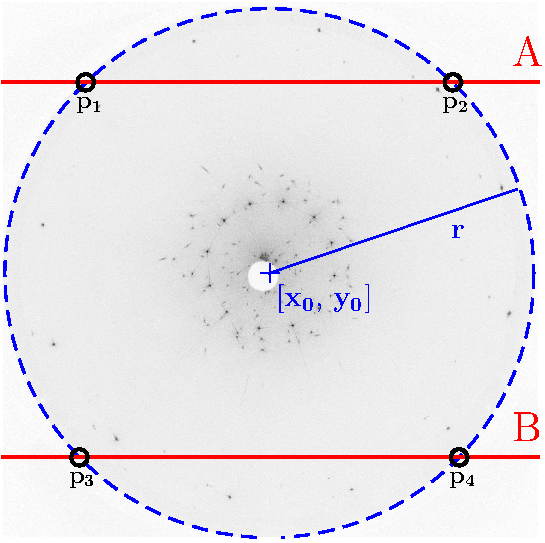
\includegraphics[width=\textwidth]{circleFit.pdf}
    \end{minipage}
    \begin{minipage}[c]{0.48\textwidth}
        \centering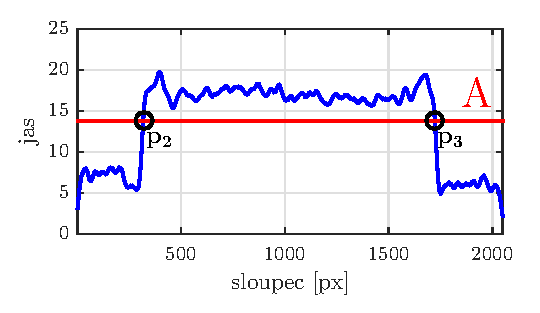
\includegraphics[width=\textwidth,height = 0.5\textwidth]{brigCutA.eps}\\
        
        \centering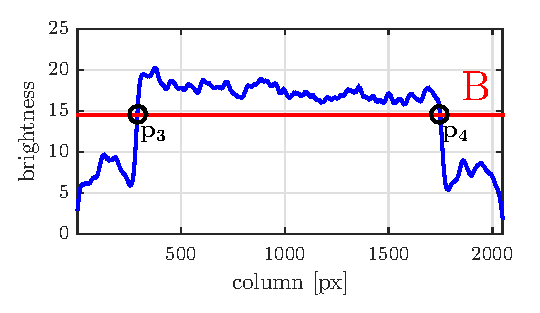
\includegraphics[width=\textwidth,height = 0.5\textwidth]{brigCutB.eps}
    \end{minipage}
    \\
        \caption[Detekce okolí stínítka.]{Jasové řezy \textit{A} a \textit{B}. Detekujeme body na kružnici $p_1$, $p_2$, $p_3$ a $p_4$. Metodou nejmenších čtverců odhadneme parametry kružnice $x_0$, $y_0$ a $R$.}
        \label{fig:CircleFit}
\end{figure}

Body na kružnici nalezeme pomocí sečen. Sečny sestrojíme ve dvou řádcích snímku. %a nalezneme sloupce, ve kterých protínáme kružnici.  
Sestrojením sečny získáme jasový řez v celé šířce snímku. Fotonový šum jasu vyfiltrujeme konvolucí s Gaussovým filtrem. Velikost filtru volíme \SI{21}{\px} a směrodatnou odchylku $\sigma = $ \SI{20}{\px}. 

Vyfiltrovaný jas oddělíme prahem. Práh určuje střední hodnota jasu v daném řezu. Nalezneme sloupce, kde je jas vyšší než prahové hodnota. Sloupec s minimálním resp. maximálním počtem pixelů určuje bod na kružnici.  

Každá sečna protíná kružnici ve dvou bodech, proto dostaneme celkem čtyři body na kružnici. Parametry kružnice určíme metodou nejmenších čtverců. 

Okolí stínítka poté definuje funkce 

\begin{equation}
	\left(x-x_0\right)^2 + \left(y-y_0\right)^2 > r^2\,.
	\label{eq:kruzniceOkoli}
	\end{equation}




\subsection{Pozadí snímku}
	V obraze nalezneme podstavec a okolí stínítka. Podstavec je specifický nízkou střední hodnotou jasu a jeho obraz je téměř ideální kruh. V seznamu MSER oblastí proto podstavec snadno nalezneme. Okolí stínítka již známe (kap. \ref{sec:okoliStinitka}).
	
	Velikost jasu v okolí stínítka nastavíme na hodnotu odvíjející se od střední hodnoty jasu snímku. Jas pixelů v oblasti podstavce nastavíme na střední hodnotu jasu pixelů v blízkém okolí podstavce.  
	
	Pozadí následně určíme konvolucí s Gaussovým filtrem. Tento filtr ignoruje vysoké změny jasu v obraze. Parametry filtru: velikost masky - \SI{201}{\px}, směrodatná odchylka $\sigma = $ \SI{201}{\px}.
	
	Samotná konvoluce s tímto filtrem by s použitím standardní funkce \textit{conv2} byla příliš časově náročná, proto konvoluci provádíme efektivnějším způsobem, který využívá rozkladu masky filtru na singulární čísla.
	
\begin{figure}[htbp]
    \centering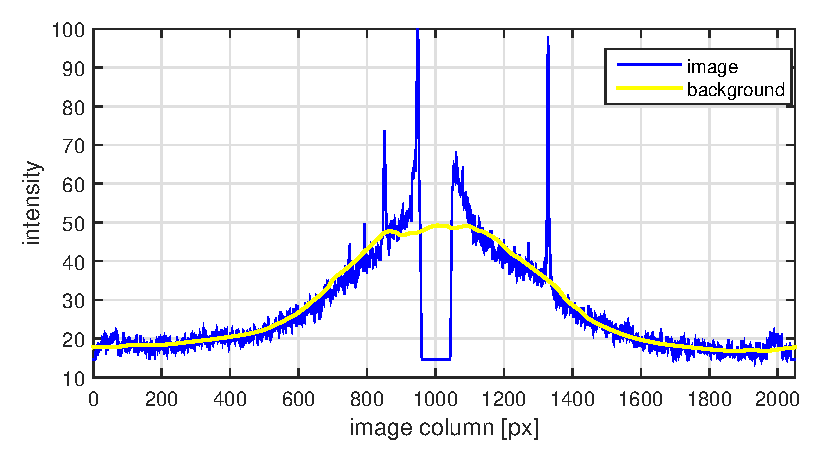
\includegraphics[width=.9\textwidth]{image_rust2.eps}
     \caption[Filtrace pozadí.]{Filtrace pozadí v HDR snímku znázorněná v řádku obrazu protínajícím obraz podstavce na kámen.}
        \label{fig:pozadi}
\end{figure}
	     
	     \newpage
\subsection{Odstranění nežádoucích detekcí}

Výstupem detektoru je soubor MSER oblastí. U výrazné světelné stopy dostaneme data ve formě pyramidy MSER oblastí podle jednotlivých úrovní intenzity. 

MSER detektor však najde nejen oblasti s výrazně vyšší intenzitou, ale i oblasti s nižší intenzitou než okolí. Ty je třeba vyřadit, protože nereprezentují světelnou stopu, kterou hledáme. 

K odstranění nežádoucích detekcí použijeme následující postup. 

\begin{enumerate}
\item Od filtrovaného snímku odečteme pozadí.

\item Ve vzniklém snímku vypočítáme střední hodnotu jasu MSER oblastí. 

\item Pokud je střední hodnota jasu záporná, MSER oblast odstraníme.  
\end{enumerate}

\section{Výsledek detekce}
Výsledky detekce světelných stop v obraze navrženého detektoru jsou srovnatelné s výstupem programu \textit{Source Extractor} \cite{SEXarticle}. Použití MSER detektoru je oproti \cite{SEXarticle} výhodné v tom, že přesně vymezuje oblast v obraze, kde se stopa nachází. Toho využíváme k určení parametrů svazků (kapitola \ref{sec:beam parameters} a \ref{sec:tails}). Ukázka detekce je na obrázku .

\begin{figure}[h!]
\centering
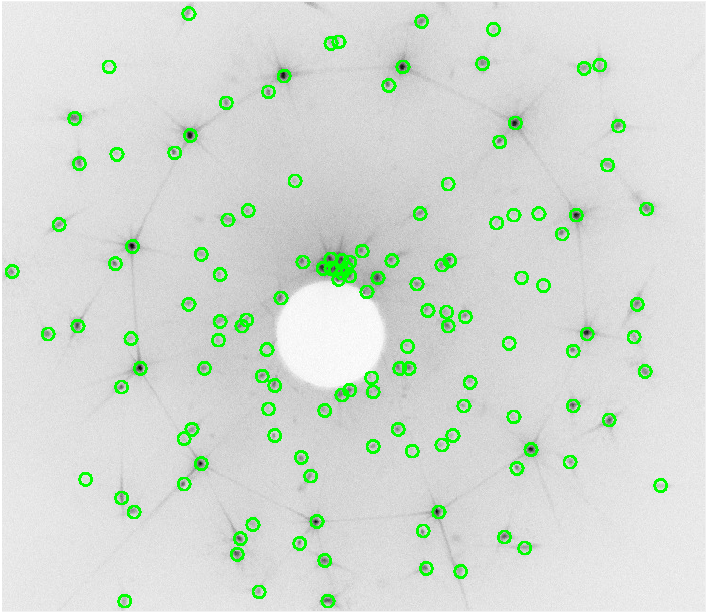
\includegraphics[width = 0.85\textwidth]{detekceVysledek.pdf}
\caption[Ukázka detekce světelných stop v obraze.]{Ukázka detekce světelných stop v obraze. }
\label{fig: podstavec}
\end{figure}

 	      

\section{Určení parametrů svazku}
\label{sec:beam parameters}
Základním parametrem svazku je směr šíření popsaný azimutem a elevací. Směr šíření svazku snadno dopočítáme, pokud nalezneme jeho obraz. Pozici světelné stopy v obraze lze určit jako polohu pixelu s maximálním jasem v detekované oblasti. Šum v obraze ale situaci komplikuje. Z obr. \ref{fig:rezy} ale vidíme, že pixel s maximálním jasem nemusí vždy určovat pozici dopadu a navíc nemusí být unikátním maximem.

Velikost obrazu měřeného svazku závisí především na jeho rozbíhavosti. Svazek od opuštění kamene do dopadu na stínítko vlivem rozbíhavosti několikanásobně zvýší svoji plochu, a proto nejsme schopni určit plochu svazku. Ze stejného důvodu nemůžeme u měřeného svazku odečítat intenzitu. Za předpokladu, že rozbíhavost svazků není příliš velká se zachová zářivý tok svazku a ten můžeme po odečtení pozadí vypočítat. %Je zřejmé, že část zářivého toku svazku se ztratí v pozadí snímku.   

V okolí obrazu svazků jsou patrné ocásky. Detekce ocásků a jejich klasifikace je popsána v samostatné kapitole \ref{sec:tails}.

Rozbíhavost svazků nemusí být ve všech směrech stejná. Na stínítku tak svazky tvoří stopy různých tvarů. Tvar stopy definujeme pomocí 3 parametrů.

\subsection{Základní parametry}

Máme detekované MSER oblasti. Nalezneme průniky oblastí a sestavíme stromovou strukturu. Kořenem stromu bude oblast s největší plochou a postupně se budou přidávat oblasti menší. Princip je patrný z 2D pohledu na prahovací úrovně MSER detektoru v obr. \ref{fig:gaussIntersection}, kde vidíme i princip tvorby stromu. Výsledkem bude řada stromů s různým počtem listů. Počet všech listů určuje počet detekovaných stop v obraze.

\begin{figure}[htbp]
    \centering
	\begin{minipage}[c]{0.78 \textwidth}
    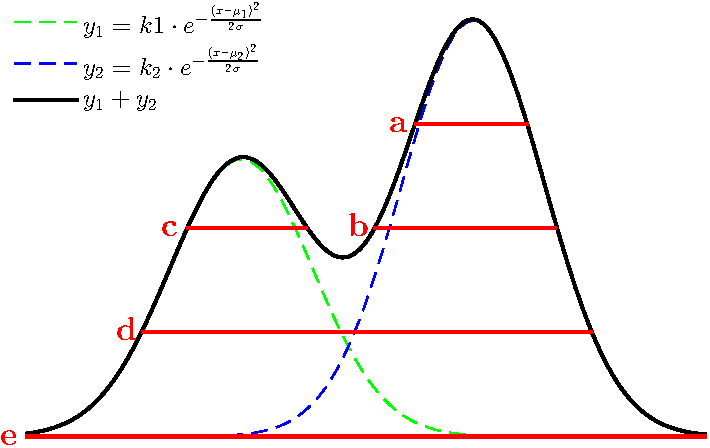
\includegraphics[width=0.95\textwidth]{gaussIntersection.pdf}
    \end{minipage}
    \begin{minipage}[c]{0.16 \textwidth}
    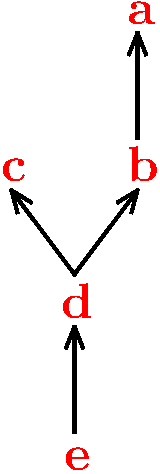
\includegraphics[width=0.95\textwidth]{treeGauss.pdf}
    \end{minipage}
    
    
     \caption[]{Ilustrace překrytí stop v 2D řezu. Výsledná charakteristika je součtem dvou Gaussových funkcí. Červeně jsou zakresleny prahovací úrovně MSER detektoru. Vlevo vidíme stromovou strukturu MSER oblastí a-f. Kořenem stromu je vrstva \textbf{e}. Vrstva \textbf{d} je jediný vnitřní uzel stromu. Listy představují vrstvy \textbf{c} a \textbf{a}. Důležité jsou podstromy \textbf{e}$\rightarrow$\textbf{d}, \textbf{c}, \textbf{b}$\rightarrow$\textbf{a}.}
        \label{fig:gaussIntersection}
\end{figure}

Cíleně prohledáváme jednotlivé stromy a nalézáme uzly, ze kterých počítáme parametry svazků.

\begin{itemize}
	\item \textbf{Azimut a elevace} - Pozici dopadu světelného svazku určíme jako střed eliptické aproximace oblasti odpovídající listu stromu. Pomocí transformace z \cite{Drapela} získáme azimut a elevaci.
	
	\item \textbf{Zářivý tok} - 
	Od filtrovaného snímku odečteme pozadí (obr. \ref{fig:pozadi}) a získáme snímek, ze kterého budeme odečítat intenzitu pixelů. Algoritmus výpočtu zářivého toku je následující:
	\begin{enumerate}
	\item $t_0$ = původní strom; $i = 0$; $q = 0$; $n_0$ = počet listů v $t_0$;
	
	\item Ve stromu $t_i$ nalezneme podstromy $\tau_1,\dots,\tau_n$ maximální velikosti bez vnitřních uzlů stromu $t_i$ a obsahující jeden list stromu $t_i$.  
	
	\item Nalezneme kořeny $\xi_1,\dots,\xi_n$ podstromů $\tau_1,\dots,\tau_n$. Kořeny odpovídají oblastem s množinou pixelů $\mathbb{M}_{q+1},\dots,\mathbb{M}_{q+n}$.
	
	\item Pokud $i = 0$ vypočítáme zářivý tok 
	
	\begin{equation}
	\underset{{k = 1}}{\sum}
	\phi_{e_j} = \frac{\underset{k\in\mathbb{M}_j}{\sum}I_k}{N_j}\,,\hspace{2cm} j\in\lbrace1,\dots,n_0\rbrace
	\end{equation}
	kde $I_k$ je jas pixelu $k$ ve snímku a $N_j$ je počet pixelů v množině $\mathbb{M}_j$. Index $j$ odpovídá indexu stopy ve stromu $t_0$.\\
	
	Pokud $i > 0$ nalezneme množiny $\mathbb{P}_1,\dots,\mathbb{P}_n$. $\mathbb{P}_l$ je množina indexů listů, které jsou v $t_0$ potomkem uzlu $\xi_l$, kde $l\in {1,\dots,n}$. Zářivý tok stop upravíme.  
	 \begin{equation}
	\phi_{e_j} = \frac{\phi_{e_j}}{\underset{q\in \mathbb{P}_l}{\sum}\phi_{e_q}}\frac{\underset{{\lbrace k\in\mathbb{M}_{q+l}\cap\lbrace \mathbb{M}_1^c \cup \mathbb{M}_2^c \cup \dots \cup \mathbb{M}_q^c \rbrace\hspace{1.5mm}|\hspace{1.5mm} \lbrace1,2,\dots,q\rbrace = \mathbb{P}_l \rbrace}}{\sum} I_k}{N_{q+l}} + \phi_{e_j}\,.\hspace{0.5cm} j\in \mathbb{P}_l
	\end{equation}
	
	\item $i = i+1$; $q = q+n$;
	\item Pokud $n \neq 1$ odstraníme podstromy $\tau_1,\dots,\tau_n$ z grafu $t_{i-1}$, získáme strom  $t_i$ a opakujeme od kroku $2$. 
	
\end{enumerate}	
	\item \textbf{Tvar} -  Pro každou MSER oblast je určena elipsa, která uzavírá danou oblast. U této elipsy lze určit orientaci a velikost hlavních poloos. 
	
	Každé stopě odpovídá jeden list stromu. Nalezneme cestu $\mathcal{C}$, která je cestou od kořene k listu. 	
	
	Orientace je určena jako medián orientací elips všech MSER oblastí v cestě $\mathcal{C}$. Velikosti hlavních poloos jsou určeny podle MSER oblasti, která je uprostřed cesty $\mathcal{C}$.		
		
\end{itemize}

\newpage
\section{Detektor ocásků}
\label{sec:tails}
	Se znalostí směru a velikosti ocásků detekovaných svazků dostáváme nové informace, které nohou přispět k jejich správnému párování se svazky z matematického modelu kamene.
	
	Ve snímaném obraze nelze rozpoznat všechny vznikající ocásky, ale pouze ty s dostatečně velkou intenzitou.

	Princip detektoru ocásků zjednodušeně spočívá v převodu okolí stopy do polárních souřadnic (vzdálenost $\rho$ a směrový úhel $\phi$) a nalezení směru, kde je patrný výrazný vzestup intenzity jasu oproti okolí. Zvýšená intenzita jasu je typicky důsledkem přítomnosti ocásku v obraze. 
	
	Abychom mohli rozvinout okolí stopy do polárního grafu, musíme si být vědomi překážek komplikující detekci ocásků.
	  
	 \begin{itemize}	 	
	 	\item V blízkém okolí jedné stopy se může nacházet další stopa. V polárním grafu se tato blízká stopa jeví jako ocásek a dochází k falešné detekci.	
	 	\item Různé stopy a ocásky mají v obraze různou velikost. Je třeba efektivně určovat vzdálenost $\rho$ do které budeme převádět okolí stopy do polárního grafu. Pokud zvolíme malé $\rho$, nepokryjeme oblast, kde se vyskytují ocásky. Příliš velké $\rho$ zvýší časovou náročnost výpočtu.   	
	 	\item Polární graf je citlivý na určení pozice dopadu svazku. 
	\end{itemize}
	
	Elegantní řešení přináší použití MSER detektoru, pomocí něhož získáme vymezení oblasti a tím i vzdálenosti $\rho$, kde se stopa i s ocásky nachází. Se znalostí oblastí náležící jednotlivým stopám jsme schopni od sebe stopy částečně oddělit a redukovat množství falešných detekcí. Na druhou stranu sousední stopa může ležet na pozici ocásku a odstraněním sousední stopy odstraníme současně i ocásek, který prozatím nejsme schopni v případě překrytí oddělit. Vzhledem k rozmanitosti stop, co do velikosti, intenzity, množství a tvaru ocásků apod. není jednoduché stopu matematicky modelovat. Pokud by se podařilo vytvořit dostatečně přesný kompaktní model stopy, je možné uvažovat o situaci, kdy budeme schopni od sebe separovat překrývající se stopy a ocásky. 
	
 Pro znázornění postupu a mezivýsledků jsme si vybrali laserovou stopu (obr. \ref{fig:mark_tail}, \ref{fig:mark_tail2}), která v obraze nekoliduje s další výraznou stopu. Zvolená stopa vznikla dopadem svazku třídy \textbf{6C}. V obraze jsou patrné čtyři ocásky různé intenzity. 
	

	\begin{figure}[h!]
	\centering
	\begin{minipage}[c]{0.35\textwidth}
	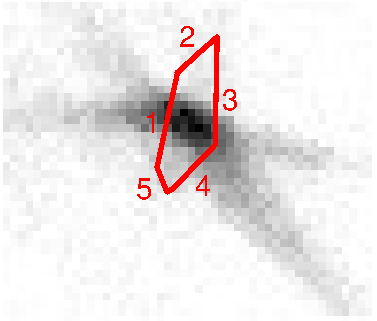
\includegraphics[width=\textwidth]{figures/tail007.pdf}
	\end{minipage}
	\begin{minipage}[c]{0.35\textwidth}
	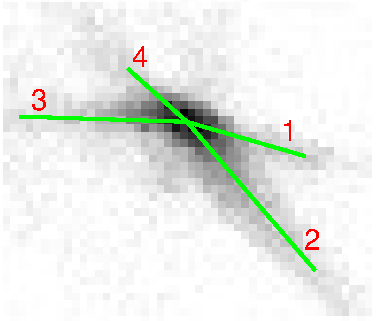
\includegraphics[width=\textwidth]{figures/tail008.pdf}
	\end{minipage}
	
	\caption[Detektor ocásků - stopa v obraze.]{Vybraná světelná stopa k ilustraci algoritmu k detekci ocásků. Stopa vznikla dopadem svazku třídy \textbf{6C} na stínítko. Vlevo: 70$\times$ zvětšený polygon simulovaného svazku. Polygon je ohraničen hranami kamene. Na hranách vznikají ocásky. Vpravo: ocásky detekované v obraze. Číslování ocásků odpovídá číslování hran na obrázku vlevo, tzn. na hraně 1 vzniká ocásek 1 atd.}
	\label{fig:mark_tail}
	\end{figure}
	



	\begin{figure}[h!]
	\centering
	\begin{minipage}[c]{0.4\textwidth}
	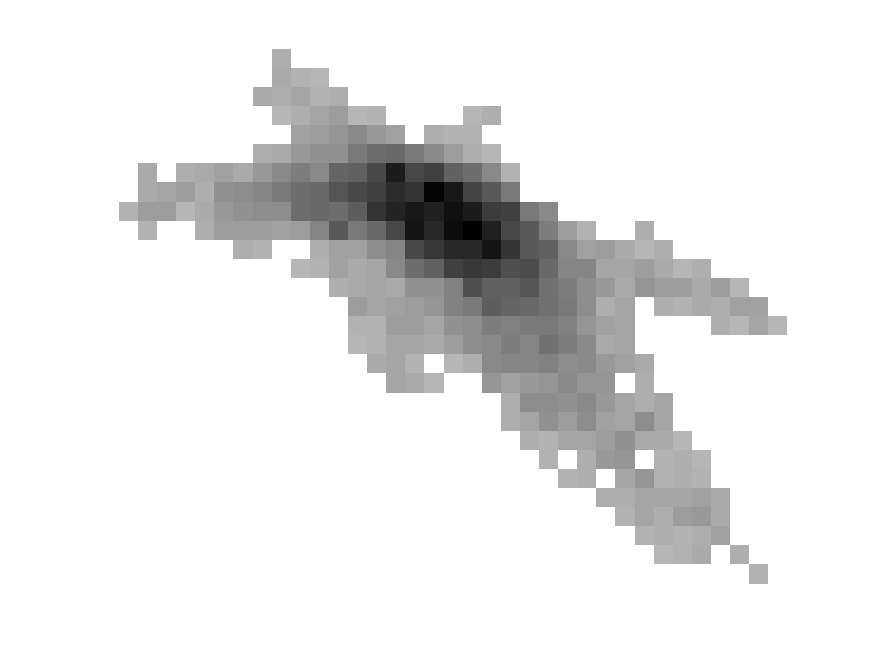
\includegraphics[width=\textwidth]{figures/tailex01.pdf}
	\end{minipage}
	\begin{minipage}[c]{0.4\textwidth}
	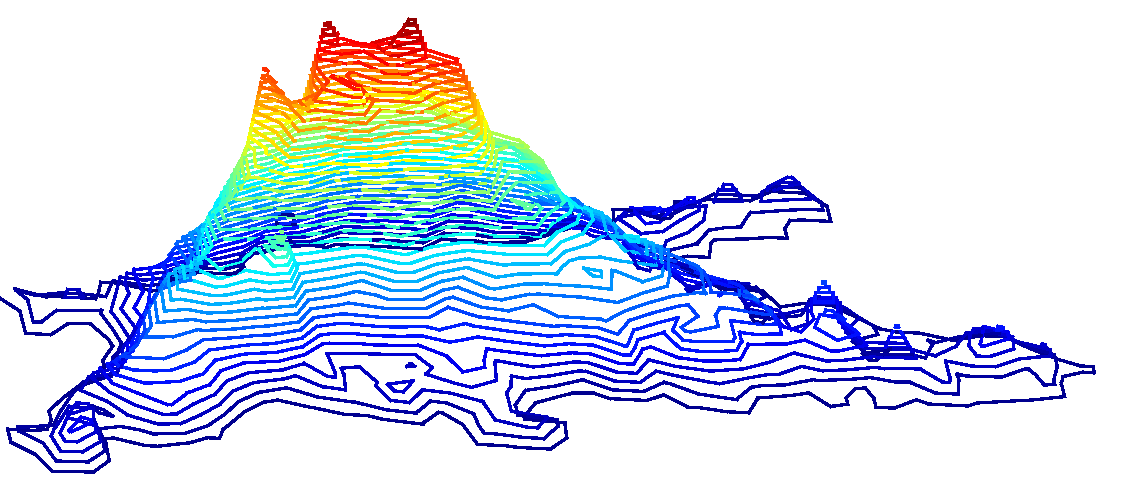
\includegraphics[width=\textwidth]{figures/tailex02.pdf}
	\end{minipage}
	
	\caption[Detektor ocásků - detekce stopy.]{Stejná světelná stopa jako na obr. \ref{fig:mark_tail}. Vpravo: detekovaná MSER oblast. Vlevo: 3D pohled na stopu.}
	\label{fig:mark_tail2}
	\end{figure}


\paragraph{Jednotlivé kroky algoritmu}

	\begin{itemize}
	\item Vybereme stopu, u které chceme identifikovat ocásky a ze snímku vybereme oblast (obr.\ref{fig:mark_tail}), která náleží zkoumané stopě. 
	
	\item U vybrané oblasti odečteme intenzitu okolí $I_o$ a vypočítáme střední hodnotu intenzity $I_m$. Intenzitu pixelů omezíme maximálně na intenzitu o velikosti $2\cdot I_m$ a potom ke všem pixelům přičteme intenzitu $I_m$. Důvodem tohoto kroku je snaha odstranit nežádoucí vlastnosti velkého šumu v hodnotách intenzity v blízkém okolí těžiště stopy a také to, že se chceme zvětšit relativní příspěvek pixelů s nižší intenzitou do součtového kritéria \ref{eq:Isuma}.   
	
	\item Oblast převedeme do polárních souřadnic ($\rho$, $\phi$). Intenzitu $I_{pol}$ v polárním grafu $I_{pol} = f(\phi,\rho)$ určujeme pomocí bipolární interpolace, která pro větší efektivitu vynechává oblasti mimo oblast stopy, kde $I_{pol} = 0$. Důležitým parametrem při interpolaci je velikost vzorkování $f_{\phi}$ úhlu $\phi$ resp. vzorkování $f_{\rho}$ vzdálenosti $\rho$ . Experimentálně jsme zvolili $f_{\phi} = \SI{3}{\degree}$ a $f_{\rho} = \SI{1}{\px}$. Interpolaci počítáme v intervalech  $\phi \in \left\langle 0,2\pi \right\rangle$ a $\rho \in \left\langle 1,\rho_{max} \right\rangle$, kde $\phi_{max}$ je maximální vzdálenost všech pixelů v oblasti stopy od její pozice.  
	
	\begin{figure}[htps]
    \centering
    \begin{minipage}[c]{0.48\textwidth}
        \centering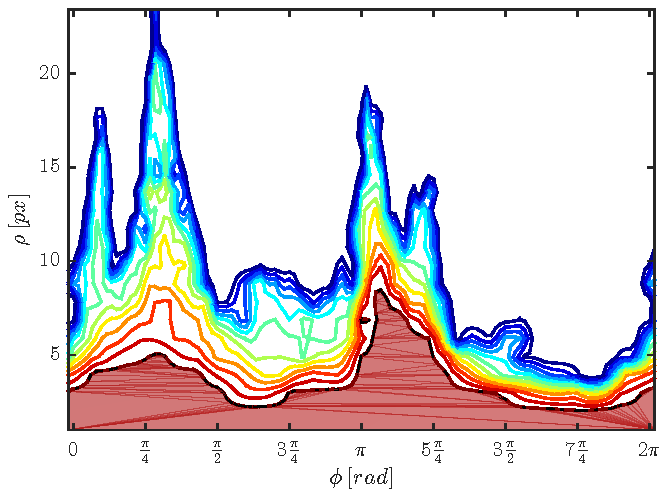
\includegraphics[width=\textwidth]{tailex03.pdf}
    \end{minipage}
    \begin{minipage}[c]{0.48\textwidth}
        \centering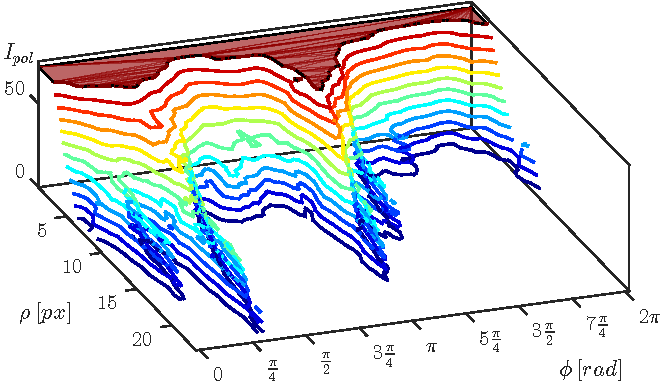
\includegraphics[width=\textwidth]{tailex04.pdf}
    \end{minipage}
    \\
        \caption[Detektor ocásků - polární graf.]{Dva pohledy na intenzitu okolí stopy převedené do polárního grafu $I_{pol}$ zobrazené pomocí vrstevnic.}
        \label{Detekce}
\end{figure}
	
	\item Provedeme součet intenzit $I_{pol}$ pro jednotlivé úhly $\phi$ od minimální do maximální vzdálenosti $\rho$ a získáme závislost $I_\phi = f(\phi)$, kde  
	
	\begin{equation}
	I_{\phi_i} = \sum_{j = 1}^{\rho_{max}} I_{pol}\left(i,j\right)\,. \hspace*{2cm} i \in \left\lbrace 0, \frac{3}{180}\pi, \dots \,,2\pi \right\rbrace
	\label{eq:Isuma}
	\end{equation}
	Následně na $I_{\phi}$ aplikujeme kubickou interpolaci sousedních hodnot s $5$krát citlivějším vzorkováním $f_{\phi_2} = \frac{f_{\phi}}{5}$ a rozšíříme rozsah $\phi$ na $\phi \in \left\langle -\frac{\pi}{2},\frac{5}{2}\pi \right\rangle$. 
	
	\item Graf závislosti $I_\phi = f(\phi)$ filtrujeme konvolucí s Gaussovou funkcí $g(x)$ se směrodatnou odchylkou $\sigma = \SI{1.2}{\degree}$ a získáme referenční závislost $I_{filt}$.
	
	\begin{equation}
		g(x) = \frac{1}{\sqrt{2\pi} \cdot \sigma}e^{-\frac{x^2}{2\sigma^2}}\,.
	\end{equation}
	
	\begin{figure}[htbp]
    \centering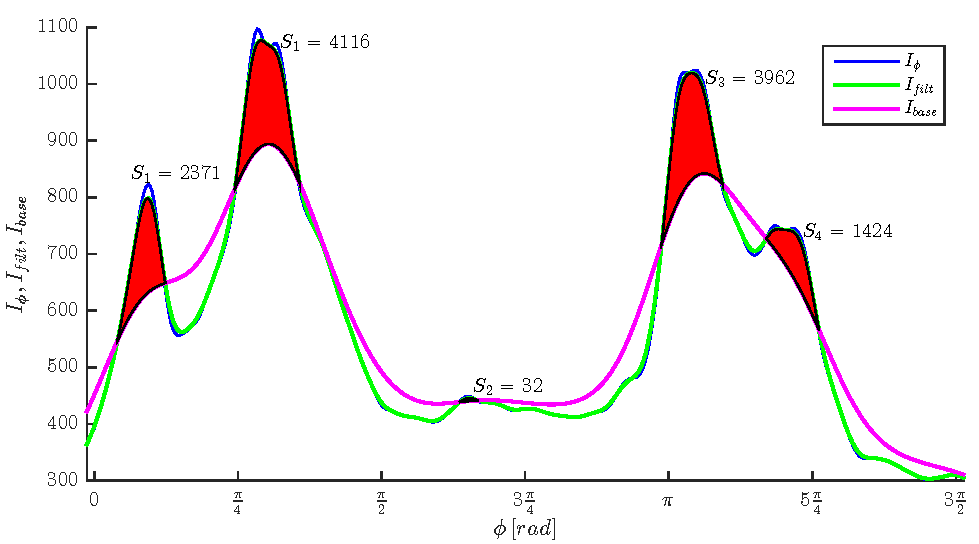
\includegraphics[width=\textwidth]{figures/tailex05.pdf}
     \caption[Detekce ocásků - zpracování polárního grafu.]{Grafické vysvětlení funkce algoritmu pro detekci ocásků. }
    \label{fig:tailSumGraph}
	\end{figure}
	
	\item Na graf $I_{filt}$ následně opakovaně aplikujeme konvoluci, tentokrát s Gaussovou funkcí $g(x)$ s vyšší směrodatnou odchylkou $\sigma = \SI{4.8}{\degree}$, abychom získali základnu $I_{base}$, kterou budeme porovnávat se signálem $I_{filt}$.
	
	\item Nalezneme souvislé oblasti $\mathcal{R}_1, \dots , \mathcal{R}_n$, kde graf $I_{filt}$ má větší hodnotu než $I_{base}$ a sečteme rozdíly $I_{filt}$ a $I_{base}$ v jednotlivých vzorcích. Velikost součtu $S_1, \dots , S_n$ závisí na vzorkovací frekvenci $f_{\phi_2}$.
	
	\begin{equation}
	S_i = \sum_{\phi_j \colon \phi_j \in \mathcal{R}_i}I_{filt}(\phi_j)-I_{base}(\phi_j)\,. \hspace*{2cm} i \in \left\lbrace 1, 2, \dots \,, n \right\rbrace
	\label{eq:Rsuma}
	\end{equation}
	
	\item Za ocásek uvažujeme oblast $\mathcal{R}_i$, kde je součet $S_i$ větší než prahovací úroveň $s_{th}$ (pro $f_{\phi_2}$ je $s_{th} = 500$). Směr ocásku $\varphi$ je určen jako úhel, ve kterém je graf $I_{filt}$ v dané oblasti maximální a velikost ocásku $\varrho_i$ určuje $\rho_{max}$ a poměr součtu $S_i$ k maximálnímu v pro danou stopu.  
	
	\begin{equation}
	\varphi_i = \argmax_{\phi_j \colon \phi_j \in \mathcal{R}_i}I_{filt}(\phi_j) \,, \hspace{1cm} \varrho_i = \frac{S_i}{\max_{j \in 1,\dots , n}S_j}\rho_{max}\,.
	\label{eq:tail_params}
	\end{equation}
		
	\begin{figure}[htbp]
    \centering
    \begin{minipage}[c]{0.48\textwidth}
        \centering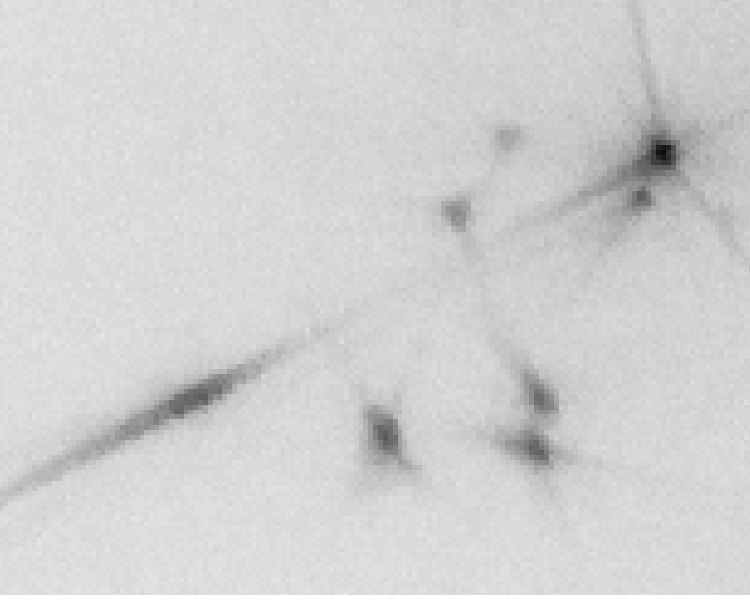
\includegraphics[width=.98\textwidth]{tail01.pdf}
    \end{minipage}
    \begin{minipage}[c]{0.48\textwidth}
        \centering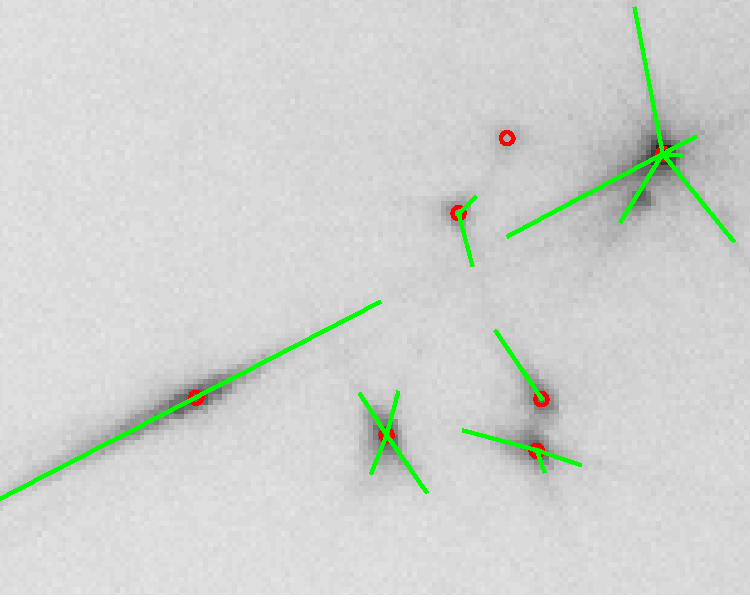
\includegraphics[width=.98\textwidth]{tail02.pdf}
    \end{minipage}
    \\
        \caption[Detektor ocásků - příklad detekce.]{Ukázka funkce detektoru ocásků na vybraném vzorku z obrazu. }
        \label{Detekce}
\end{figure}
	
\end{itemize}	   
	
	

%\section{MSER detector configuration parameter list}	
%	Here is a list of the configuration parameters used for beam detection setting. All of them can be used with their default values. This description of the parameters can be usefull for understanding the algorithm or debugging.
%	
%\begin{center}
%
%
%\begin{tabular}{l|l|p{8cm}}
%    \textbf{Name} 		& \textbf{Default} & \textbf{Description} \\ \hline \hline 
%    \textit{BackgroundFilt}	    	& $201$ 	& Size of Gaussian filter mask used for background estimation. \textit{Sigma} of mask is equal to \textit{BackgroundFilt} \\ \hline
%    \textit{BackgroundKMean}    	& $0.15$	& $BackgroundKMean \times mean(image)$ is added to background estimation. \\ \hline
%    \textit{ComputeAllLayers}   	& $1$		& $1$ - Divide all layers in marks variable calculation. $0$ - Calculate only with upper layers. \\ \hline
%    \textit{ComputeTails}   		& $ 1 $		& $1$ - Tails of marks are computed. It takes some time. $0$ - No tails. Faster.\\ \hline    
%    \textit{CleanerAxisRatio}   	& $ 10 $	& MSER regions with upper axis ratio are deleted. \\ \hline
%    \textit{CleanerFilterSigma}  	& $ 5 $		& \textit{Sigma} of filter mask in image blurring. \\ \hline
%    \textit{CleanerFilterSize}   	& $ 31 $	& Size of filter mask in image blurring.\\ \hline
%	\textit{CleanerMean}    		& $ 0.035 $ & Regions with peak where difference of mean of surrounding
%intensity is lower than $CleanerMean \times mean(image)$ are deleted. \\ \hline
%    \textit{CleanerSumWide} 		& $ 5 $		& Size of surrounding in cleaning process.  \\ \hline
%    \textit{FilterSigma}    		& $ 0.7 $	& \textit{Sigma} of niose reducing filter mask. \\ \hline
%    \textit{FilterSize} 			& $ 3 $		& \textit{Size} of niose reducing filter mask.\\ \hline 
%    \textit{MSERMaxAreaVar} 		& $ 0.9 $	& This value specifies the step size between intensity threshold levels used in selecting extremal regions while testing for their stability. Decrease this value to return more regions.\\ \hline
%    \textit{MSERRegion} 			&$[2\,,\, 14000]$& Two-element vector, [minArea maxArea], which specifies the size of the regions in pixels. This value allows the selection of regions containing pixels between minArea and maxArea, inclusive.\\ \hline
%    \textit{MSERThresh} 			& $ 1.2 $	& Increase this value to return a greater number of regions at the cost of their stability. Stable regions are very similar in size over varying intensity thresholds.\\ \hline
%    \textit{SurroundThres}   		& $ 0.8 $	& Multiple of $mean(image)$ where surrounding intensity is moved.   \\ 
%\end{tabular}
%
%\end{center}

\clearpage
\subsection{Parametry kamene \textit{viva12}}

Šatonová růže má 14 rovinných faset. Fasety označujeme zkratkami \textbf{TOP}, \textbf{BOT} a \textbf{UF1-UF12}, kde

\begin{tabular}{l l}
\textbf{TOP} & - tabulka,\\
\textbf{BOT} & - spodek,\\
\textbf{UF1-UF12} & - 12 bočních faset.\\
\end{tabular}\\

Označené fasety máme na obrázku \ref{fig:viva12Params} spolu s vyznačenými parametry

\begin{tabular}{l l}
$d_{TOP}$ & průměr tabulky,\\
$d_{BOT}$ & průměr spodku,\\
$h$ & výška kamene,\\
$h_{RF}$ & výška lemu. 
\end{tabular}\\
 
Poznamenejme, že lem modelujeme množstvím faset, které po spojení aproximují oválný tvar. Tyto fasety mají v simulaci absorpční charakter. Světelné svazky, které na ně dopadnou, zaniknou.   

\begin{figure}[htps]
\centering
\begin{minipage}[c]{0.4\textwidth}
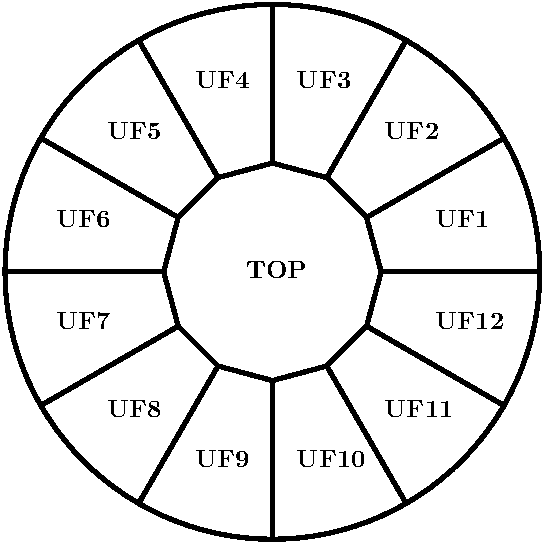
\includegraphics[width=\textwidth]{vivi12Facets1.pdf}
\end{minipage}
\begin{minipage}[c]{0.56\textwidth}
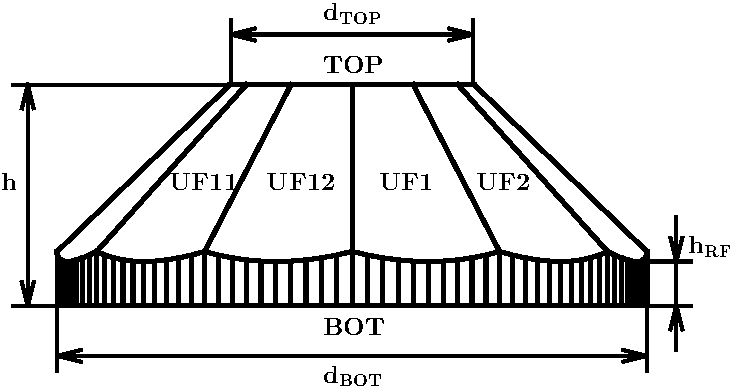
\includegraphics[width=\textwidth]{vivi12Facets2.pdf}
\end{minipage}
\caption{Šatonová růže s označenými fasetami a parametry. Pohled shora je zobrazen vlevo, bokorys vpravo.}
\label{fig:viva12Params}
\end{figure}

\subsection{Klasifikace svazků do tříd}
Typ svazku definujeme podle pořadí dopadových faset. Při opakovaném použití ovšem tento způsob popisu není přehledný.

 Pro lepší orientaci si svazky rozdělíme do tříd a budeme pracovat pouze s jejím názvem. Název je u všech tříd dvouciferný.
 
  První cifra udává počet dopadových faset. Zde se pohybujeme od 1 do 9. Svazky s větším počtem dopadových faset než 9 nejsme schopni na stínítku rozpoznat a definovat je nemá smysl. 
  
  Na pozici druhé cifry se objevují znaky abecedy \textit{A-Z}. Svazky s jednotným počtem odrazů se začínají značit od písmene \textit{A} a to tak, že \textit{A} patří třídě svazků, která má největší zářivý tok. Zářivý tok třídy svazků postupně klesá s abecedním pořadím. Svazky, které nemají dostatečný zářivý tok a nelze je spařit na stínítku neuvádíme. 
  
  Svazky popisujeme pro situaci, kdy směrový vektor zdrojového svazku je přibližně kolmý k rovině spodku. Pokud bychom kámen orientovali jinak, řada tříd by přestala existovat a zároveň by se objevily i nové nepopsané třídy. 
  
  Rozdělení svazků do tříd je zapsáno v tabulkách \ref{table:TableClasses1}, \ref{table:TableClasses2}, \ref{table:TableClasses3}, \ref{table:TableClasses4}, \ref{table:TableClasses5} a \ref{table:TableClasses6}.
  
  
 
 
  


\begin{table}[h!]
\centering
\begin{tabular}{|l|c|c|c|c|c|c|c|c|c|c|c|c|}
\hline
Class &  \multicolumn{9}{l}{Ray path} \vline  & Count\\
\hline \hline
\textbf{1A} & UF1 & UF2 & UF3 & UF4 & UF5 & UF6 & UF7 & UF8 & $\dots$ & 12\\
\hline \hline
\textbf{1B} & \multicolumn{9}{l}{TOP} \vline  & 1\\
\hline \hline
\textbf{3A} & UF1 & UF2 & UF3 & UF4 & UF5 & UF6 & UF7 & UF8 & $\dots$ & 12\\
 & BOT & BOT & BOT & BOT & BOT & BOT & BOT & BOT & $\dots$ & \\
 & TOP & TOP & TOP & TOP & TOP & TOP & TOP & TOP & $\dots$ & \\
\hline \hline
\textbf{3B} & \multicolumn{9}{l}{TOP-BOT-TOP} \vline  & 1\\
\hline \hline
\textbf{5A} & UF1 & UF2 & UF3 & UF4 & UF5 & UF6 & UF7 & UF8 & $\dots$ & 12\\
 & BOT & BOT & BOT & BOT & BOT & BOT & BOT & BOT & $\dots$ & \\
 & TOP & TOP & TOP & TOP & TOP & TOP & TOP & TOP & $\dots$ & \\
 & BOT & BOT & BOT & BOT & BOT & BOT & BOT & BOT & $\dots$ & \\
 & UF6 & UF7 & UF8 & UF9 & UF10 & UF11 & UF12 & UF1 & $\dots$ & \\
\hline \hline
\textbf{5B} & UF1 & UF2 & UF3 & UF4 & UF5 & UF6 & UF7 & UF8 & $\dots$ & 12\\
 & BOT & BOT & BOT & BOT & BOT & BOT & BOT & BOT & $\dots$ & \\
 & TOP & TOP & TOP & TOP & TOP & TOP & TOP & TOP & $\dots$ & \\
 & BOT & BOT & BOT & BOT & BOT & BOT & BOT & BOT & $\dots$ & \\
 & UF7 & UF8 & UF9 & UF10 & UF11 & UF12 & UF1 & UF2 & $\dots$ & \\
\hline \hline
\textbf{5C} & UF1 & UF2 & UF3 & UF4 & UF5 & UF6 & UF7 & UF8 & $\dots$ & 12\\
 & BOT & BOT & BOT & BOT & BOT & BOT & BOT & BOT & $\dots$ & \\
 & TOP & TOP & TOP & TOP & TOP & TOP & TOP & TOP & $\dots$ & \\
 & BOT & BOT & BOT & BOT & BOT & BOT & BOT & BOT & $\dots$ & \\
 & UF8 & UF9 & UF10 & UF11 & UF12 & UF1 & UF2 & UF3 & $\dots$ & \\
\hline \hline
\textbf{5D} & UF1 & UF2 & UF3 & UF4 & UF5 & UF6 & UF7 & UF8 & $\dots$ & 12\\
 & BOT & BOT & BOT & BOT & BOT & BOT & BOT & BOT & $\dots$ & \\
 & TOP & TOP & TOP & TOP & TOP & TOP & TOP & TOP & $\dots$ & \\
 & BOT & BOT & BOT & BOT & BOT & BOT & BOT & BOT & $\dots$ & \\
 & TOP & TOP & TOP & TOP & TOP & TOP & TOP & TOP & $\dots$ & \\
\hline \hline
\textbf{5E} & \multicolumn{9}{l}{TOP-BOT-TOP-BOT-TOP} \vline  & 1\\
\hline \hline
\textbf{6A} & UF1 & UF2 & UF3 & UF4 & UF5 & UF6 & UF7 & UF8 & $\dots$ & 12\\
 & BOT & BOT & BOT & BOT & BOT & BOT & BOT & BOT & $\dots$ & \\
 & UF1 & UF2 & UF3 & UF4 & UF5 & UF6 & UF7 & UF8 & $\dots$ & \\
 & UF6 & UF7 & UF8 & UF9 & UF10 & UF11 & UF12 & UF1 & $\dots$ & \\
 & BOT & BOT & BOT & BOT & BOT & BOT & BOT & BOT & $\dots$ & \\
 & UF8 & UF9 & UF10 & UF11 & UF12 & UF1 & UF2 & UF3 & $\dots$ & \\
\hline \hline
\textbf{6B} & UF1 & UF2 & UF3 & UF4 & UF5 & UF6 & UF7 & UF8 & $\dots$ & 12\\
 & BOT & BOT & BOT & BOT & BOT & BOT & BOT & BOT & $\dots$ & \\
 & UF12 & UF1 & UF2 & UF3 & UF4 & UF5 & UF6 & UF7 & $\dots$ & \\
 & UF6 & UF7 & UF8 & UF9 & UF10 & UF11 & UF12 & UF1 & $\dots$ & \\
 & BOT & BOT & BOT & BOT & BOT & BOT & BOT & BOT & $\dots$ & \\
 & UF7 & UF8 & UF9 & UF10 & UF11 & UF12 & UF1 & UF2 & $\dots$ & \\
\hline \hline
\textbf{6C} & UF1 & UF2 & UF3 & UF4 & UF5 & UF6 & UF7 & UF8 & $\dots$ & 12\\
 & BOT & BOT & BOT & BOT & BOT & BOT & BOT & BOT & $\dots$ & \\
 & UF2 & UF3 & UF4 & UF5 & UF6 & UF7 & UF8 & UF9 & $\dots$ & \\
 & UF8 & UF9 & UF10 & UF11 & UF12 & UF1 & UF2 & UF3 & $\dots$ & \\
 & BOT & BOT & BOT & BOT & BOT & BOT & BOT & BOT & $\dots$ & \\
 & UF7 & UF8 & UF9 & UF10 & UF11 & UF12 & UF1 & UF2 & $\dots$ & \\
\hline 
\end{tabular}
\caption{Paths of rays with count of rays in class. Classes 1A-6C.}
\label{table:TableClasses1}
\end{table}




\begin{table}[h!]
\centering
\begin{tabular}{|l|c|c|c|c|c|c|c|c|c|c|c|c|}
\hline
Class &  \multicolumn{9}{l}{Ray path} \vline  & Count\\
\hline \hline
\textbf{6D} & UF1 & UF2 & UF3 & UF4 & UF5 & UF6 & UF7 & UF8 & $\dots$ & 12\\
 & BOT & BOT & BOT & BOT & BOT & BOT & BOT & BOT & $\dots$ & \\
 & UF1 & UF2 & UF3 & UF4 & UF5 & UF6 & UF7 & UF8 & $\dots$ & \\
 & UF8 & UF9 & UF10 & UF11 & UF12 & UF1 & UF2 & UF3 & $\dots$ & \\
 & BOT & BOT & BOT & BOT & BOT & BOT & BOT & BOT & $\dots$ & \\
 & UF6 & UF7 & UF8 & UF9 & UF10 & UF11 & UF12 & UF1 & $\dots$ & \\
\hline \hline
\textbf{6E} & TOP & TOP & TOP & TOP & TOP & TOP & TOP & TOP & $\dots$ & 12\\
 & BOT & BOT & BOT & BOT & BOT & BOT & BOT & BOT & $\dots$ & \\
 & UF2 & UF3 & UF4 & UF5 & UF6 & UF7 & UF8 & UF9 & $\dots$ & \\
 & UF8 & UF9 & UF10 & UF11 & UF12 & UF1 & UF2 & UF3 & $\dots$ & \\
 & BOT & BOT & BOT & BOT & BOT & BOT & BOT & BOT & $\dots$ & \\
 & UF8 & UF9 & UF10 & UF11 & UF12 & UF1 & UF2 & UF3 & $\dots$ & \\
\hline \hline
\textbf{6F} & UF1 & UF2 & UF3 & UF4 & UF5 & UF6 & UF7 & UF8 & $\dots$ & 12\\
 & BOT & BOT & BOT & BOT & BOT & BOT & BOT & BOT & $\dots$ & \\
 & UF1 & UF2 & UF3 & UF4 & UF5 & UF6 & UF7 & UF8 & $\dots$ & \\
 & UF7 & UF8 & UF9 & UF10 & UF11 & UF12 & UF1 & UF2 & $\dots$ & \\
 & BOT & BOT & BOT & BOT & BOT & BOT & BOT & BOT & $\dots$ & \\
 & TOP & TOP & TOP & TOP & TOP & TOP & TOP & TOP & $\dots$ & \\
\hline \hline
\textbf{7A} & UF1 & UF2 & UF3 & UF4 & UF5 & UF6 & UF7 & UF8 & $\dots$ & 12\\
 & BOT & BOT & BOT & BOT & BOT & BOT & BOT & BOT & $\dots$ & \\
 & UF1 & UF2 & UF3 & UF4 & UF5 & UF6 & UF7 & UF8 & $\dots$ & \\
 & TOP & TOP & TOP & TOP & TOP & TOP & TOP & TOP & $\dots$ & \\
 & UF6 & UF7 & UF8 & UF9 & UF10 & UF11 & UF12 & UF1 & $\dots$ & \\
 & BOT & BOT & BOT & BOT & BOT & BOT & BOT & BOT & $\dots$ & \\
 & UF7 & UF8 & UF9 & UF10 & UF11 & UF12 & UF1 & UF2 & $\dots$ & \\
\hline \hline
\textbf{7B} & UF1 & UF2 & UF3 & UF4 & UF5 & UF6 & UF7 & UF8 & $\dots$ & 12\\
 & BOT & BOT & BOT & BOT & BOT & BOT & BOT & BOT & $\dots$ & \\
 & UF1 & UF2 & UF3 & UF4 & UF5 & UF6 & UF7 & UF8 & $\dots$ & \\
 & TOP & TOP & TOP & TOP & TOP & TOP & TOP & TOP & $\dots$ & \\
 & UF8 & UF9 & UF10 & UF11 & UF12 & UF1 & UF2 & UF3 & $\dots$ & \\
 & BOT & BOT & BOT & BOT & BOT & BOT & BOT & BOT & $\dots$ & \\
 & UF7 & UF8 & UF9 & UF10 & UF11 & UF12 & UF1 & UF2 & $\dots$ & \\
\hline \hline
\textbf{7C} & UF1 & UF2 & UF3 & UF4 & UF5 & UF6 & UF7 & UF8 & $\dots$ & 12\\
 & BOT & BOT & BOT & BOT & BOT & BOT & BOT & BOT & $\dots$ & \\
 & UF1 & UF2 & UF3 & UF4 & UF5 & UF6 & UF7 & UF8 & $\dots$ & \\
 & TOP & TOP & TOP & TOP & TOP & TOP & TOP & TOP & $\dots$ & \\
 & UF7 & UF8 & UF9 & UF10 & UF11 & UF12 & UF1 & UF2 & $\dots$ & \\
 & BOT & BOT & BOT & BOT & BOT & BOT & BOT & BOT & $\dots$ & \\
 & UF7 & UF8 & UF9 & UF10 & UF11 & UF12 & UF1 & UF2 & $\dots$ & \\
\hline \hline
\textbf{7D} & UF1 & UF2 & UF3 & UF4 & UF5 & UF6 & UF7 & UF8 & $\dots$ & 12\\
 & BOT & BOT & BOT & BOT & BOT & BOT & BOT & BOT & $\dots$ & \\
 & UF2 & UF3 & UF4 & UF5 & UF6 & UF7 & UF8 & UF9 & $\dots$ & \\
 & TOP & TOP & TOP & TOP & TOP & TOP & TOP & TOP & $\dots$ & \\
 & UF8 & UF9 & UF10 & UF11 & UF12 & UF1 & UF2 & UF3 & $\dots$ & \\
 & BOT & BOT & BOT & BOT & BOT & BOT & BOT & BOT & $\dots$ & \\
 & UF7 & UF8 & UF9 & UF10 & UF11 & UF12 & UF1 & UF2 & $\dots$ & \\
\hline 
\end{tabular}
\caption{Paths of rays with count of rays in class. Classes 6D-7D.}
\label{table:TableClasses2}
\end{table}

\begin{table}[h!]
\centering
\begin{tabular}{|l|c|c|c|c|c|c|c|c|c|c|c|c|}
\hline
Class &  \multicolumn{9}{l}{Ray path} \vline  & Count\\
\hline \hline
\textbf{7E} & UF1 & UF2 & UF3 & UF4 & UF5 & UF6 & UF7 & UF8 & $\dots$ & 12\\
 & BOT & BOT & BOT & BOT & BOT & BOT & BOT & BOT & $\dots$ & \\
 & UF2 & UF3 & UF4 & UF5 & UF6 & UF7 & UF8 & UF9 & $\dots$ & \\
 & TOP & TOP & TOP & TOP & TOP & TOP & TOP & TOP & $\dots$ & \\
 & UF8 & UF9 & UF10 & UF11 & UF12 & UF1 & UF2 & UF3 & $\dots$ & \\
 & BOT & BOT & BOT & BOT & BOT & BOT & BOT & BOT & $\dots$ & \\
 & UF8 & UF9 & UF10 & UF11 & UF12 & UF1 & UF2 & UF3 & $\dots$ & \\
\hline \hline
\textbf{7F} & UF1 & UF2 & UF3 & UF4 & UF5 & UF6 & UF7 & UF8 & $\dots$ & 12\\
 & BOT & BOT & BOT & BOT & BOT & BOT & BOT & BOT & $\dots$ & \\
 & UF12 & UF1 & UF2 & UF3 & UF4 & UF5 & UF6 & UF7 & $\dots$ & \\
 & TOP & TOP & TOP & TOP & TOP & TOP & TOP & TOP & $\dots$ & \\
 & UF6 & UF7 & UF8 & UF9 & UF10 & UF11 & UF12 & UF1 & $\dots$ & \\
 & BOT & BOT & BOT & BOT & BOT & BOT & BOT & BOT & $\dots$ & \\
 & UF6 & UF7 & UF8 & UF9 & UF10 & UF11 & UF12 & UF1 & $\dots$ & \\
\hline \hline
\textbf{7G} & UF1 & UF2 & UF3 & UF4 & UF5 & UF6 & UF7 & UF8 & $\dots$ & 12\\
 & BOT & BOT & BOT & BOT & BOT & BOT & BOT & BOT & $\dots$ & \\
 & UF12 & UF1 & UF2 & UF3 & UF4 & UF5 & UF6 & UF7 & $\dots$ & \\
 & TOP & TOP & TOP & TOP & TOP & TOP & TOP & TOP & $\dots$ & \\
 & UF6 & UF7 & UF8 & UF9 & UF10 & UF11 & UF12 & UF1 & $\dots$ & \\
 & BOT & BOT & BOT & BOT & BOT & BOT & BOT & BOT & $\dots$ & \\
 & UF7 & UF8 & UF9 & UF10 & UF11 & UF12 & UF1 & UF2 & $\dots$ & \\
\hline \hline
\textbf{7H} & \multicolumn{9}{l}{TOP-BOT-TOP-BOT-TOP-BOT-TOP} \vline  & 1\\
\hline \hline
\textbf{8A} & UF1 & UF2 & UF3 & UF4 & UF5 & UF6 & UF7 & UF8 & $\dots$ & 12\\
 & BOT & BOT & BOT & BOT & BOT & BOT & BOT & BOT & $\dots$ & \\
 & UF1 & UF2 & UF3 & UF4 & UF5 & UF6 & UF7 & UF8 & $\dots$ & \\
 & UF8 & UF9 & UF10 & UF11 & UF12 & UF1 & UF2 & UF3 & $\dots$ & \\
 & BOT & BOT & BOT & BOT & BOT & BOT & BOT & BOT & $\dots$ & \\
 & UF6 & UF7 & UF8 & UF9 & UF10 & UF11 & UF12 & UF1 & $\dots$ & \\
 & BOT & BOT & BOT & BOT & BOT & BOT & BOT & BOT & $\dots$ & \\
 & UF1 & UF2 & UF3 & UF4 & UF5 & UF6 & UF7 & UF8 & $\dots$ & \\
\hline \hline
\textbf{8B} & UF1 & UF2 & UF3 & UF4 & UF5 & UF6 & UF7 & UF8 & $\dots$ & 12\\
 & BOT & BOT & BOT & BOT & BOT & BOT & BOT & BOT & $\dots$ & \\
 & UF1 & UF2 & UF3 & UF4 & UF5 & UF6 & UF7 & UF8 & $\dots$ & \\
 & UF6 & UF7 & UF8 & UF9 & UF10 & UF11 & UF12 & UF1 & $\dots$ & \\
 & BOT & BOT & BOT & BOT & BOT & BOT & BOT & BOT & $\dots$ & \\
 & UF8 & UF9 & UF10 & UF11 & UF12 & UF1 & UF2 & UF3 & $\dots$ & \\
 & BOT & BOT & BOT & BOT & BOT & BOT & BOT & BOT & $\dots$ & \\
 & UF12 & UF1 & UF2 & UF3 & UF4 & UF5 & UF6 & UF7 & $\dots$ & \\
\hline \hline
\textbf{8C} & UF1 & UF2 & UF3 & UF4 & UF5 & UF6 & UF7 & UF8 & $\dots$ & 12\\
 & BOT & BOT & BOT & BOT & BOT & BOT & BOT & BOT & $\dots$ & \\
 & UF1 & UF2 & UF3 & UF4 & UF5 & UF6 & UF7 & UF8 & $\dots$ & \\
 & UF6 & UF7 & UF8 & UF9 & UF10 & UF11 & UF12 & UF1 & $\dots$ & \\
 & BOT & BOT & BOT & BOT & BOT & BOT & BOT & BOT & $\dots$ & \\
 & UF8 & UF9 & UF10 & UF11 & UF12 & UF1 & UF2 & UF3 & $\dots$ & \\
 & BOT & BOT & BOT & BOT & BOT & BOT & BOT & BOT & $\dots$ & \\
 & UF1 & UF2 & UF3 & UF4 & UF5 & UF6 & UF7 & UF8 & $\dots$ & \\
\hline 
\end{tabular}
\caption{Paths of rays with count of rays in class. Classes 7E-8C.}
\label{table:TableClasses3}
\end{table}


\begin{table}[h!]
\centering
\begin{tabular}{|l|c|c|c|c|c|c|c|c|c|c|c|c|}
\hline
Class &  \multicolumn{9}{l}{Ray path} \vline  & Count\\
\hline \hline
\textbf{8D} & UF1 & UF2 & UF3 & UF4 & UF5 & UF6 & UF7 & UF8 & $\dots$ & 12\\
 & BOT & BOT & BOT & BOT & BOT & BOT & BOT & BOT & $\dots$ & \\
 & UF1 & UF2 & UF3 & UF4 & UF5 & UF6 & UF7 & UF8 & $\dots$ & \\
 & UF8 & UF9 & UF10 & UF11 & UF12 & UF1 & UF2 & UF3 & $\dots$ & \\
 & BOT & BOT & BOT & BOT & BOT & BOT & BOT & BOT & $\dots$ & \\
 & UF6 & UF7 & UF8 & UF9 & UF10 & UF11 & UF12 & UF1 & $\dots$ & \\
 & BOT & BOT & BOT & BOT & BOT & BOT & BOT & BOT & $\dots$ & \\
 & UF2 & UF3 & UF4 & UF5 & UF6 & UF7 & UF8 & UF9 & $\dots$ & \\
\hline \hline
\textbf{9A} & UF6 & UF7 & UF8 & UF9 & UF10 & UF11 & UF12 & UF1 & $\dots$ & 12\\
 & BOT & BOT & BOT & BOT & BOT & BOT & BOT & BOT & $\dots$ & \\
 & UF6 & UF7 & UF8 & UF9 & UF10 & UF11 & UF12 & UF1 & $\dots$ & \\
 & TOP & TOP & TOP & TOP & TOP & TOP & TOP & TOP & $\dots$ & \\
 & UF12 & UF1 & UF2 & UF3 & UF4 & UF5 & UF6 & UF7 & $\dots$ & \\
 & BOT & BOT & BOT & BOT & BOT & BOT & BOT & BOT & $\dots$ & \\
 & UF12 & UF1 & UF2 & UF3 & UF4 & UF5 & UF6 & UF7 & $\dots$ & \\
 & BOT & BOT & BOT & BOT & BOT & BOT & BOT & BOT & $\dots$ & \\
 & UF6 & UF7 & UF8 & UF9 & UF10 & UF11 & UF12 & UF1 & $\dots$ & \\
\hline \hline
\textbf{9B} & UF1 & UF2 & UF3 & UF4 & UF5 & UF6 & UF7 & UF8 & $\dots$ & 12\\
 & BOT & BOT & BOT & BOT & BOT & BOT & BOT & BOT & $\dots$ & \\
 & UF1 & UF2 & UF3 & UF4 & UF5 & UF6 & UF7 & UF8 & $\dots$ & \\
 & UF7 & UF8 & UF9 & UF10 & UF11 & UF12 & UF1 & UF2 & $\dots$ & \\
 & BOT & BOT & BOT & BOT & BOT & BOT & BOT & BOT & $\dots$ & \\
 & UF8 & UF9 & UF10 & UF11 & UF12 & UF1 & UF2 & UF3 & $\dots$ & \\
 & UF2 & UF3 & UF4 & UF5 & UF6 & UF7 & UF8 & UF9 & $\dots$ & \\
 & BOT & BOT & BOT & BOT & BOT & BOT & BOT & BOT & $\dots$ & \\
 & UF2 & UF3 & UF4 & UF5 & UF6 & UF7 & UF8 & UF9 & $\dots$ & \\
\hline \hline
\textbf{9C} & UF1 & UF2 & UF3 & UF4 & UF5 & UF6 & UF7 & UF8 & $\dots$ & 12\\
 & BOT & BOT & BOT & BOT & BOT & BOT & BOT & BOT & $\dots$ & \\
 & UF1 & UF2 & UF3 & UF4 & UF5 & UF6 & UF7 & UF8 & $\dots$ & \\
 & UF7 & UF8 & UF9 & UF10 & UF11 & UF12 & UF1 & UF2 & $\dots$ & \\
 & BOT & BOT & BOT & BOT & BOT & BOT & BOT & BOT & $\dots$ & \\
 & UF7 & UF8 & UF9 & UF10 & UF11 & UF12 & UF1 & UF2 & $\dots$ & \\
 & UF1 & UF2 & UF3 & UF4 & UF5 & UF6 & UF7 & UF8 & $\dots$ & \\
 & BOT & BOT & BOT & BOT & BOT & BOT & BOT & BOT & $\dots$ & \\
 & UF1 & UF2 & UF3 & UF4 & UF5 & UF6 & UF7 & UF8 & $\dots$ & \\
\hline \hline
\textbf{9D} & UF1 & UF2 & UF3 & UF4 & UF5 & UF6 & UF7 & UF8 & $\dots$ & 12\\
 & BOT & BOT & BOT & BOT & BOT & BOT & BOT & BOT & $\dots$ & \\
 & UF1 & UF2 & UF3 & UF4 & UF5 & UF6 & UF7 & UF8 & $\dots$ & \\
 & UF7 & UF8 & UF9 & UF10 & UF11 & UF12 & UF1 & UF2 & $\dots$ & \\
 & BOT & BOT & BOT & BOT & BOT & BOT & BOT & BOT & $\dots$ & \\
 & UF6 & UF7 & UF8 & UF9 & UF10 & UF11 & UF12 & UF1 & $\dots$ & \\
 & UF12 & UF1 & UF2 & UF3 & UF4 & UF5 & UF6 & UF7 & $\dots$ & \\
 & BOT & BOT & BOT & BOT & BOT & BOT & BOT & BOT & $\dots$ & \\
 & UF12 & UF1 & UF2 & UF3 & UF4 & UF5 & UF6 & UF7 & $\dots$ & \\
\hline 
\end{tabular}
\caption{Paths of rays with count of rays in class. Classes 8D-9D.}
\label{table:TableClasses4}
\end{table}

\begin{table}[h!]
\centering
\begin{tabular}{|l|c|c|c|c|c|c|c|c|c|c|c|c|}
\hline
Class &  \multicolumn{9}{l}{Ray path} \vline  & Count\\
\hline \hline
\textbf{9E} & UF1 & UF2 & UF3 & UF4 & UF5 & UF6 & UF7 & UF8 & $\dots$ & 12\\
 & BOT & BOT & BOT & BOT & BOT & BOT & BOT & BOT & $\dots$ & \\
 & UF2 & UF3 & UF4 & UF5 & UF6 & UF7 & UF8 & UF9 & $\dots$ & \\
 & UF8 & UF9 & UF10 & UF11 & UF12 & UF1 & UF2 & UF3 & $\dots$ & \\
 & BOT & BOT & BOT & BOT & BOT & BOT & BOT & BOT & $\dots$ & \\
 & UF7 & UF8 & UF9 & UF10 & UF11 & UF12 & UF1 & UF2 & $\dots$ & \\
 & UF1 & UF2 & UF3 & UF4 & UF5 & UF6 & UF7 & UF8 & $\dots$ & \\
 & BOT & BOT & BOT & BOT & BOT & BOT & BOT & BOT & $\dots$ & \\
 & UF1 & UF2 & UF3 & UF4 & UF5 & UF6 & UF7 & UF8 & $\dots$ & \\
\hline \hline
\textbf{9F} & UF1 & UF2 & UF3 & UF4 & UF5 & UF6 & UF7 & UF8 & $\dots$ & 12\\
 & BOT & BOT & BOT & BOT & BOT & BOT & BOT & BOT & $\dots$ & \\
 & UF2 & UF3 & UF4 & UF5 & UF6 & UF7 & UF8 & UF9 & $\dots$ & \\
 & UF8 & UF9 & UF10 & UF11 & UF12 & UF1 & UF2 & UF3 & $\dots$ & \\
 & BOT & BOT & BOT & BOT & BOT & BOT & BOT & BOT & $\dots$ & \\
 & UF7 & UF8 & UF9 & UF10 & UF11 & UF12 & UF1 & UF2 & $\dots$ & \\
 & UF1 & UF2 & UF3 & UF4 & UF5 & UF6 & UF7 & UF8 & $\dots$ & \\
 & BOT & BOT & BOT & BOT & BOT & BOT & BOT & BOT & $\dots$ & \\
 & UF2 & UF3 & UF4 & UF5 & UF6 & UF7 & UF8 & UF9 & $\dots$ & \\
\hline \hline
\textbf{9G} & UF1 & UF2 & UF3 & UF4 & UF5 & UF6 & UF7 & UF8 & $\dots$ & 12\\
 & BOT & BOT & BOT & BOT & BOT & BOT & BOT & BOT & $\dots$ & \\
 & UF2 & UF3 & UF4 & UF5 & UF6 & UF7 & UF8 & UF9 & $\dots$ & \\
 & UF8 & UF9 & UF10 & UF11 & UF12 & UF1 & UF2 & UF3 & $\dots$ & \\
 & BOT & BOT & BOT & BOT & BOT & BOT & BOT & BOT & $\dots$ & \\
 & UF7 & UF8 & UF9 & UF10 & UF11 & UF12 & UF1 & UF2 & $\dots$ & \\
 & UF2 & UF3 & UF4 & UF5 & UF6 & UF7 & UF8 & UF9 & $\dots$ & \\
 & BOT & BOT & BOT & BOT & BOT & BOT & BOT & BOT & $\dots$ & \\
 & UF1 & UF2 & UF3 & UF4 & UF5 & UF6 & UF7 & UF8 & $\dots$ & \\
\hline \hline
\textbf{9H} & UF1 & UF2 & UF3 & UF4 & UF5 & UF6 & UF7 & UF8 & $\dots$ & 12\\
 & BOT & BOT & BOT & BOT & BOT & BOT & BOT & BOT & $\dots$ & \\
 & UF12 & UF1 & UF2 & UF3 & UF4 & UF5 & UF6 & UF7 & $\dots$ & \\
 & UF6 & UF7 & UF8 & UF9 & UF10 & UF11 & UF12 & UF1 & $\dots$ & \\
 & BOT & BOT & BOT & BOT & BOT & BOT & BOT & BOT & $\dots$ & \\
 & UF7 & UF8 & UF9 & UF10 & UF11 & UF12 & UF1 & UF2 & $\dots$ & \\
 & UF1 & UF2 & UF3 & UF4 & UF5 & UF6 & UF7 & UF8 & $\dots$ & \\
 & BOT & BOT & BOT & BOT & BOT & BOT & BOT & BOT & $\dots$ & \\
 & UF1 & UF2 & UF3 & UF4 & UF5 & UF6 & UF7 & UF8 & $\dots$ & \\
\hline \hline
\textbf{9I} & UF1 & UF2 & UF3 & UF4 & UF5 & UF6 & UF7 & UF8 & $\dots$ & 12\\
 & BOT & BOT & BOT & BOT & BOT & BOT & BOT & BOT & $\dots$ & \\
 & UF12 & UF1 & UF2 & UF3 & UF4 & UF5 & UF6 & UF7 & $\dots$ & \\
 & UF6 & UF7 & UF8 & UF9 & UF10 & UF11 & UF12 & UF1 & $\dots$ & \\
 & BOT & BOT & BOT & BOT & BOT & BOT & BOT & BOT & $\dots$ & \\
 & UF7 & UF8 & UF9 & UF10 & UF11 & UF12 & UF1 & UF2 & $\dots$ & \\
 & UF1 & UF2 & UF3 & UF4 & UF5 & UF6 & UF7 & UF8 & $\dots$ & \\
 & BOT & BOT & BOT & BOT & BOT & BOT & BOT & BOT & $\dots$ & \\
 & UF12 & UF1 & UF2 & UF3 & UF4 & UF5 & UF6 & UF7 & $\dots$ & \\
\hline 
\end{tabular}
\caption{Paths of rays with count of rays in class. Classes 9E-9I.}
\label{table:TableClasses5}
\end{table}

\clearpage

\begin{table}[h!]
\centering
\begin{tabular}{|l|c|c|c|c|c|c|c|c|c|c|c|c|}
\hline
Class &  \multicolumn{9}{l}{Ray path} \vline  & Count\\
\hline \hline
\textbf{9J} & UF1 & UF2 & UF3 & UF4 & UF5 & UF6 & UF7 & UF8 & $\dots$ & 12\\
 & BOT & BOT & BOT & BOT & BOT & BOT & BOT & BOT & $\dots$ & \\
 & UF12 & UF1 & UF2 & UF3 & UF4 & UF5 & UF6 & UF7 & $\dots$ & \\
 & UF6 & UF7 & UF8 & UF9 & UF10 & UF11 & UF12 & UF1 & $\dots$ & \\
 & BOT & BOT & BOT & BOT & BOT & BOT & BOT & BOT & $\dots$ & \\
 & UF7 & UF8 & UF9 & UF10 & UF11 & UF12 & UF1 & UF2 & $\dots$ & \\
 & UF12 & UF1 & UF2 & UF3 & UF4 & UF5 & UF6 & UF7 & $\dots$ & \\
 & BOT & BOT & BOT & BOT & BOT & BOT & BOT & BOT & $\dots$ & \\
 & UF1 & UF2 & UF3 & UF4 & UF5 & UF6 & UF7 & UF8 & $\dots$ & \\
\hline 
\end{tabular}
\caption{Paths of rays with count of rays in class 9J.}
\label{table:TableClasses6}
\end{table}


\begin{figure}[htps]
\centering
\begin{minipage}[c]{0.325\textwidth}
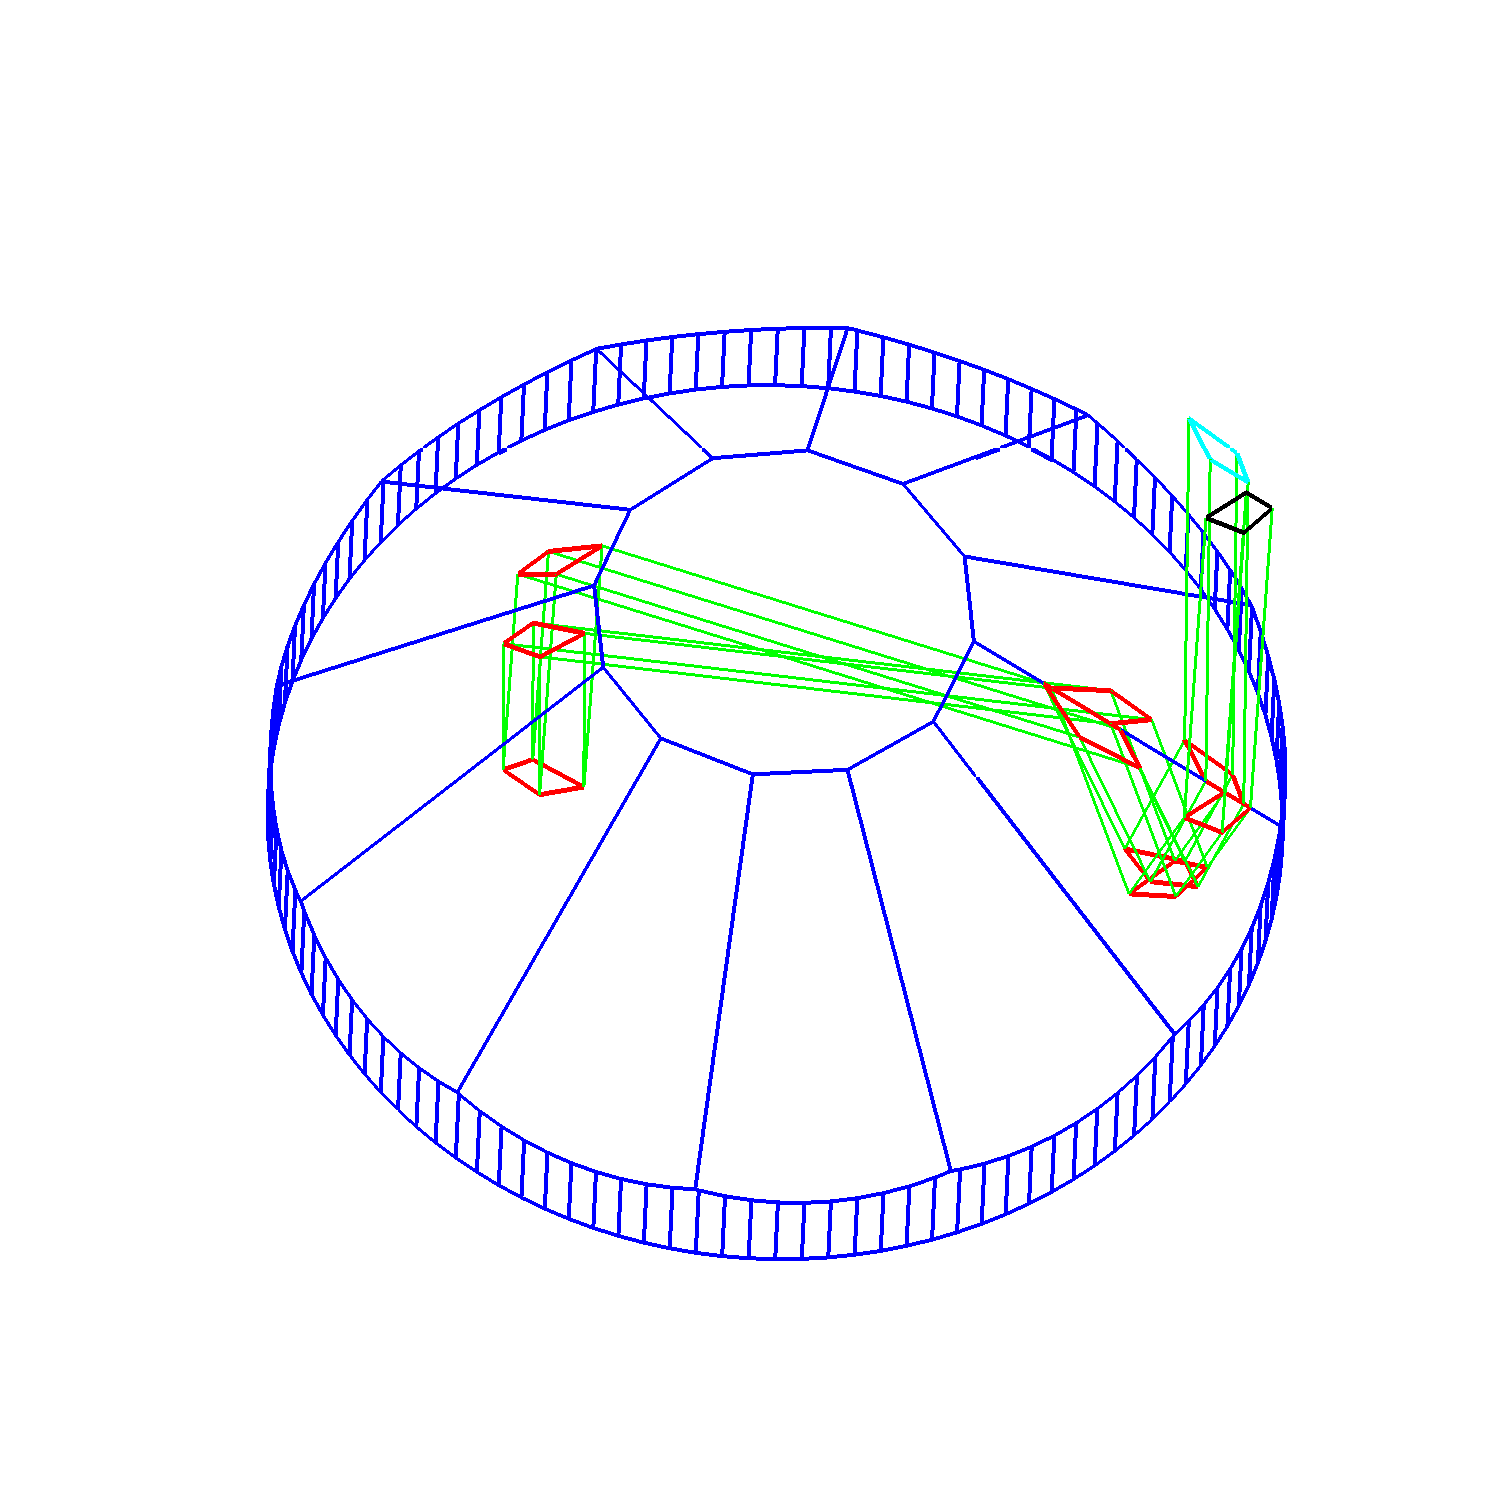
\includegraphics[width=\textwidth]{group9I.pdf}
\end{minipage}
\caption{3D view of ray example in classes 9J.}
\label{fig:modelClass3D1}
\end{figure}


\begin{figure}[htps]
\centering
\begin{minipage}[c]{0.325\textwidth}
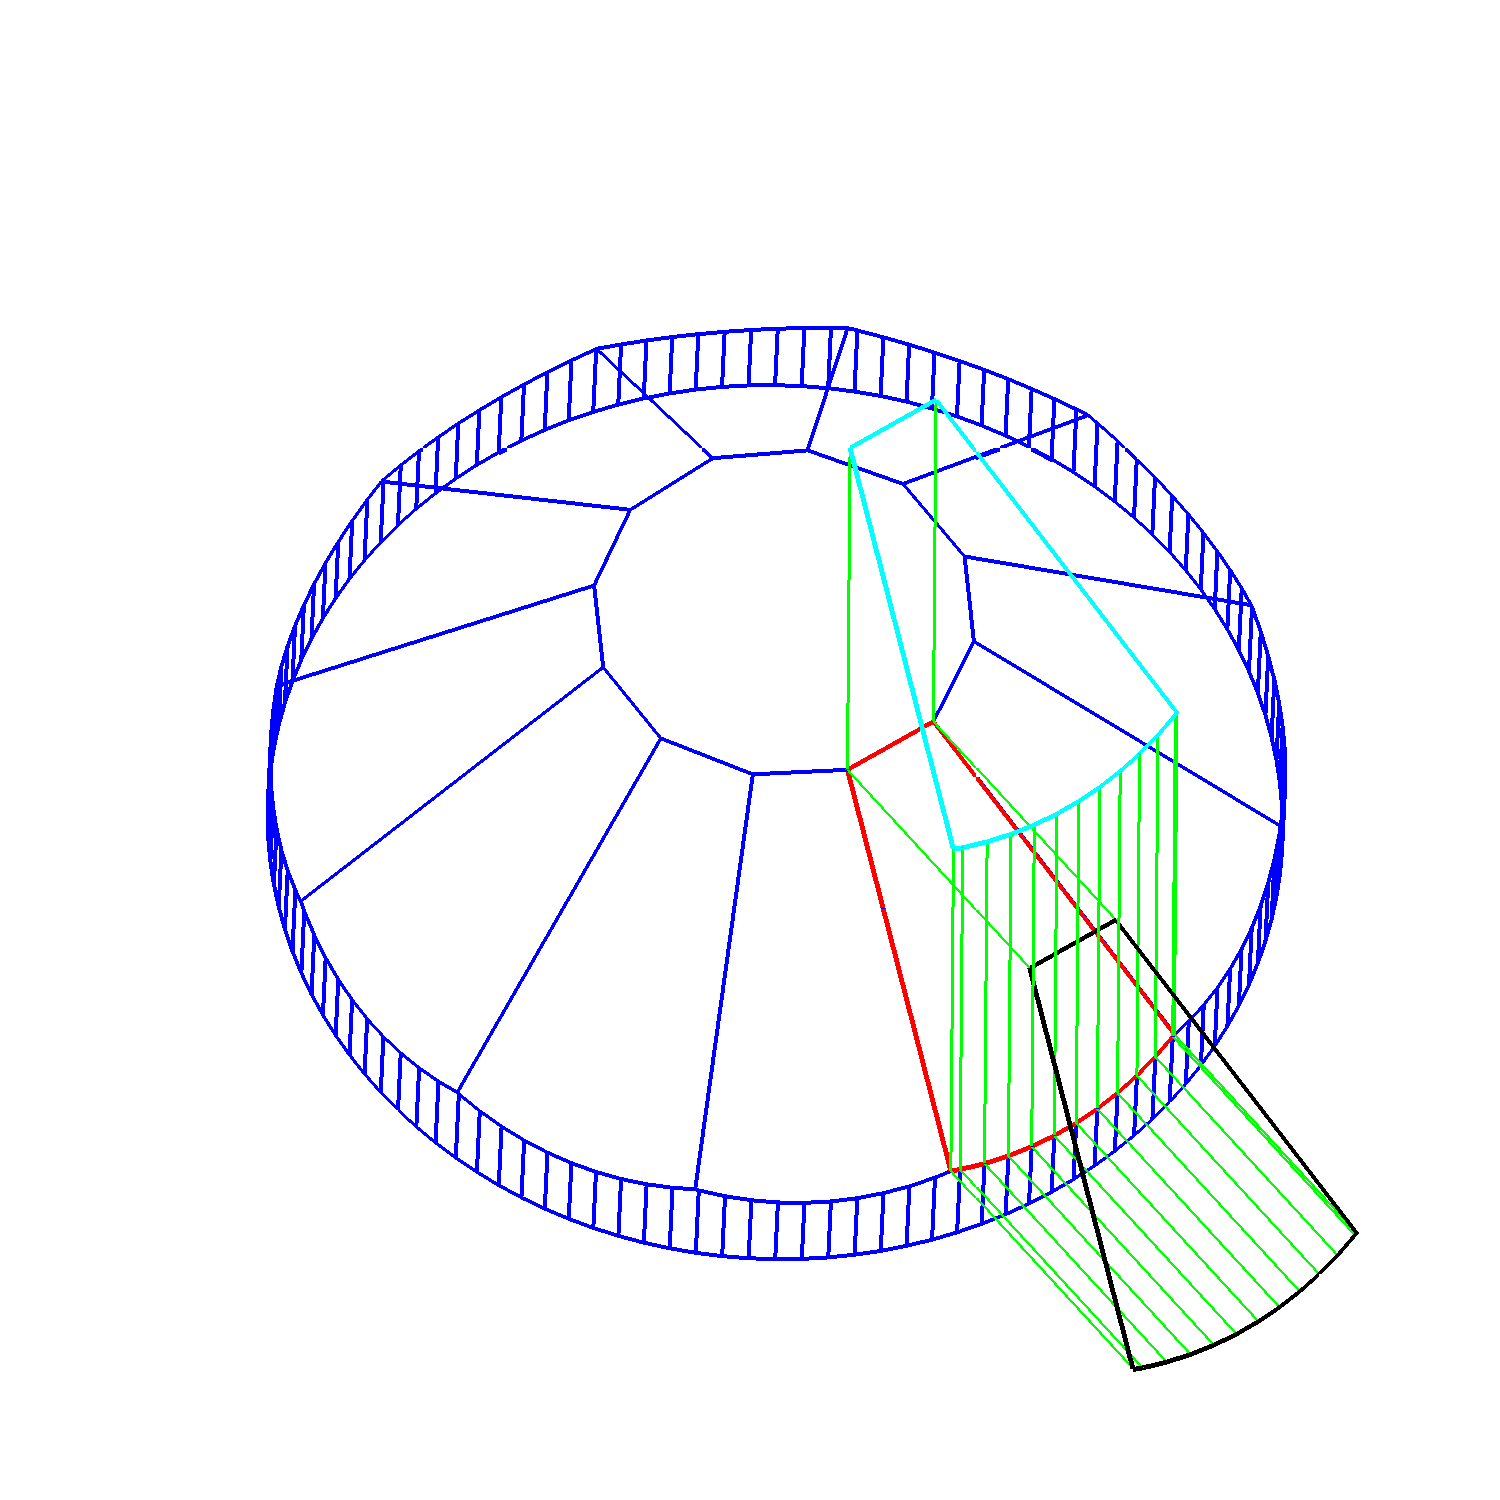
\includegraphics[width=\textwidth]{group1A.pdf}
\end{minipage}
\begin{minipage}[c]{0.325\textwidth}
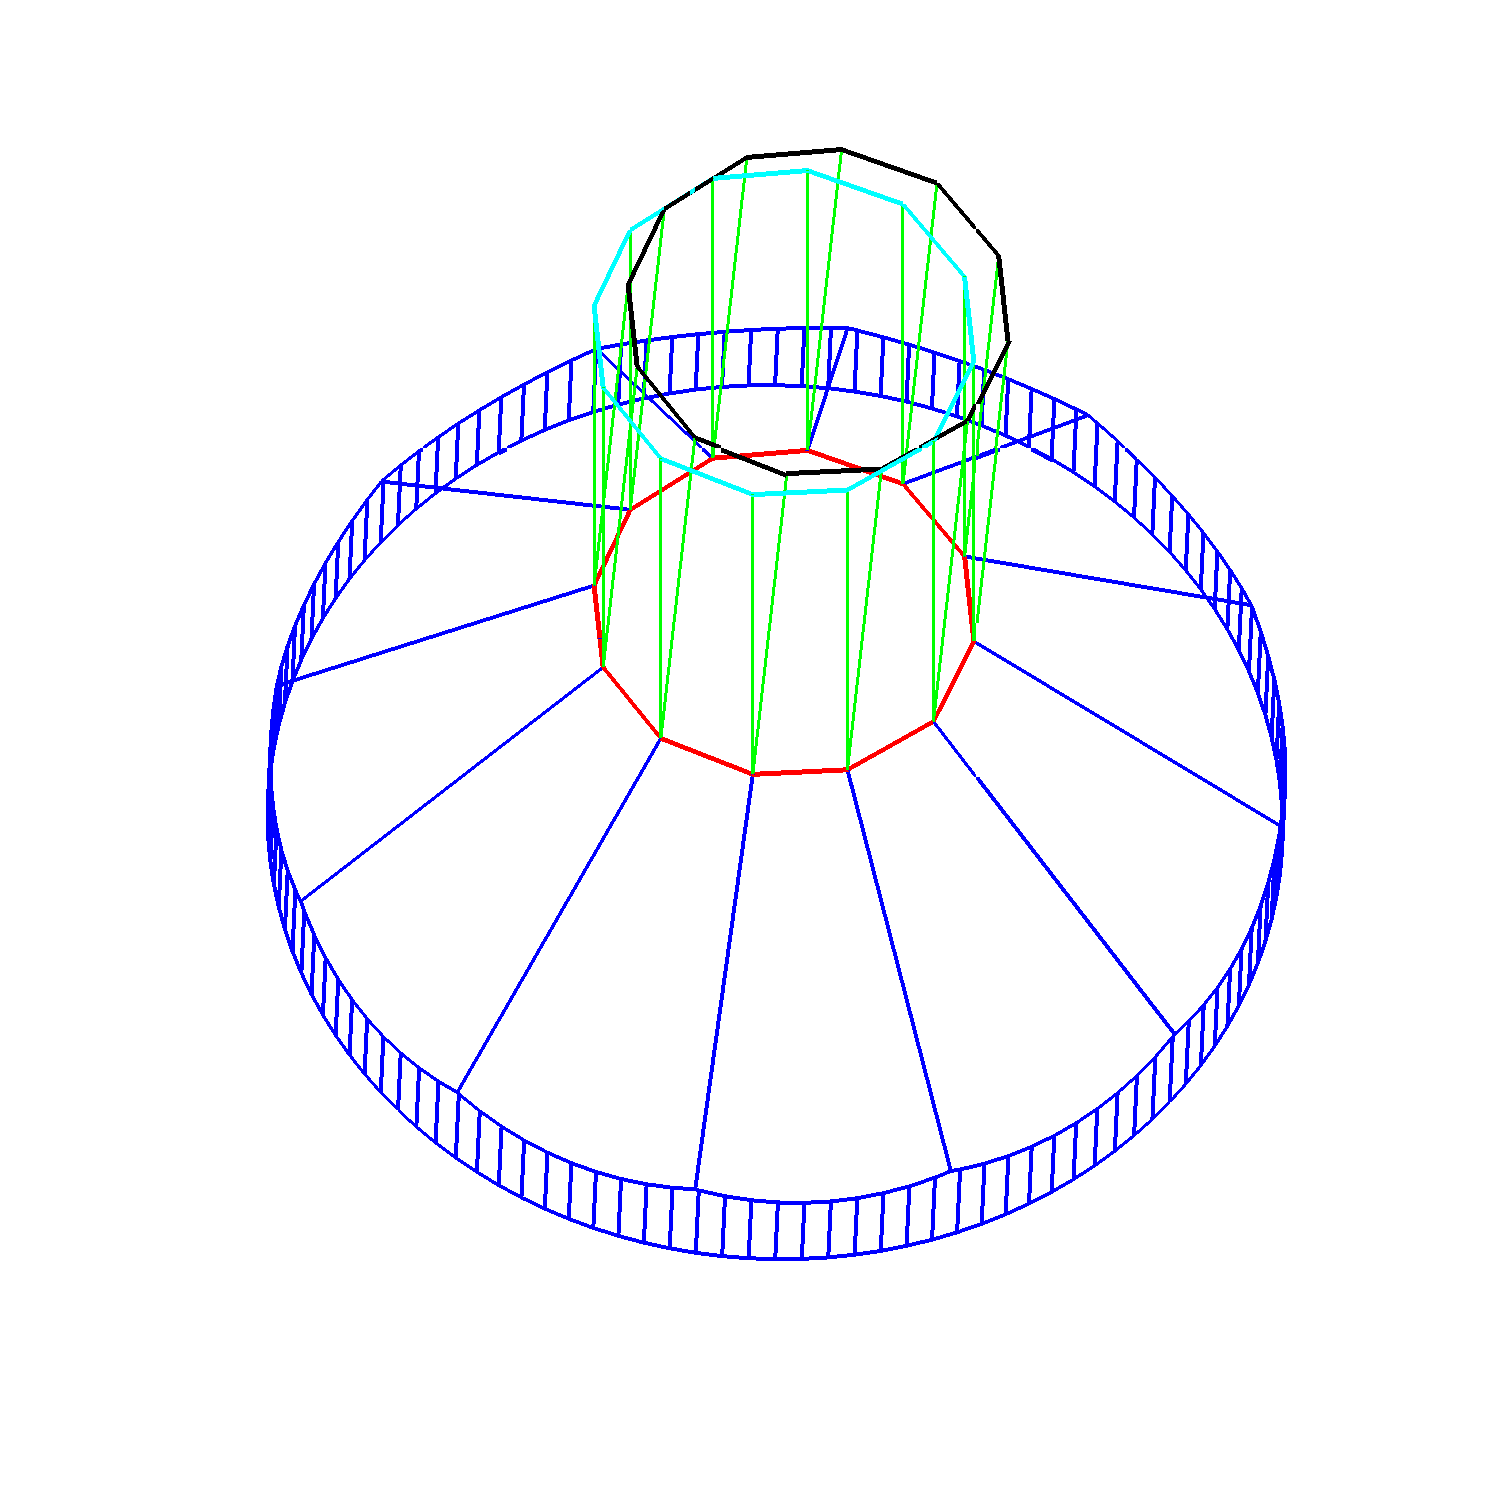
\includegraphics[width=\textwidth]{group1B.pdf}
\end{minipage}
\begin{minipage}[c]{0.325\textwidth}
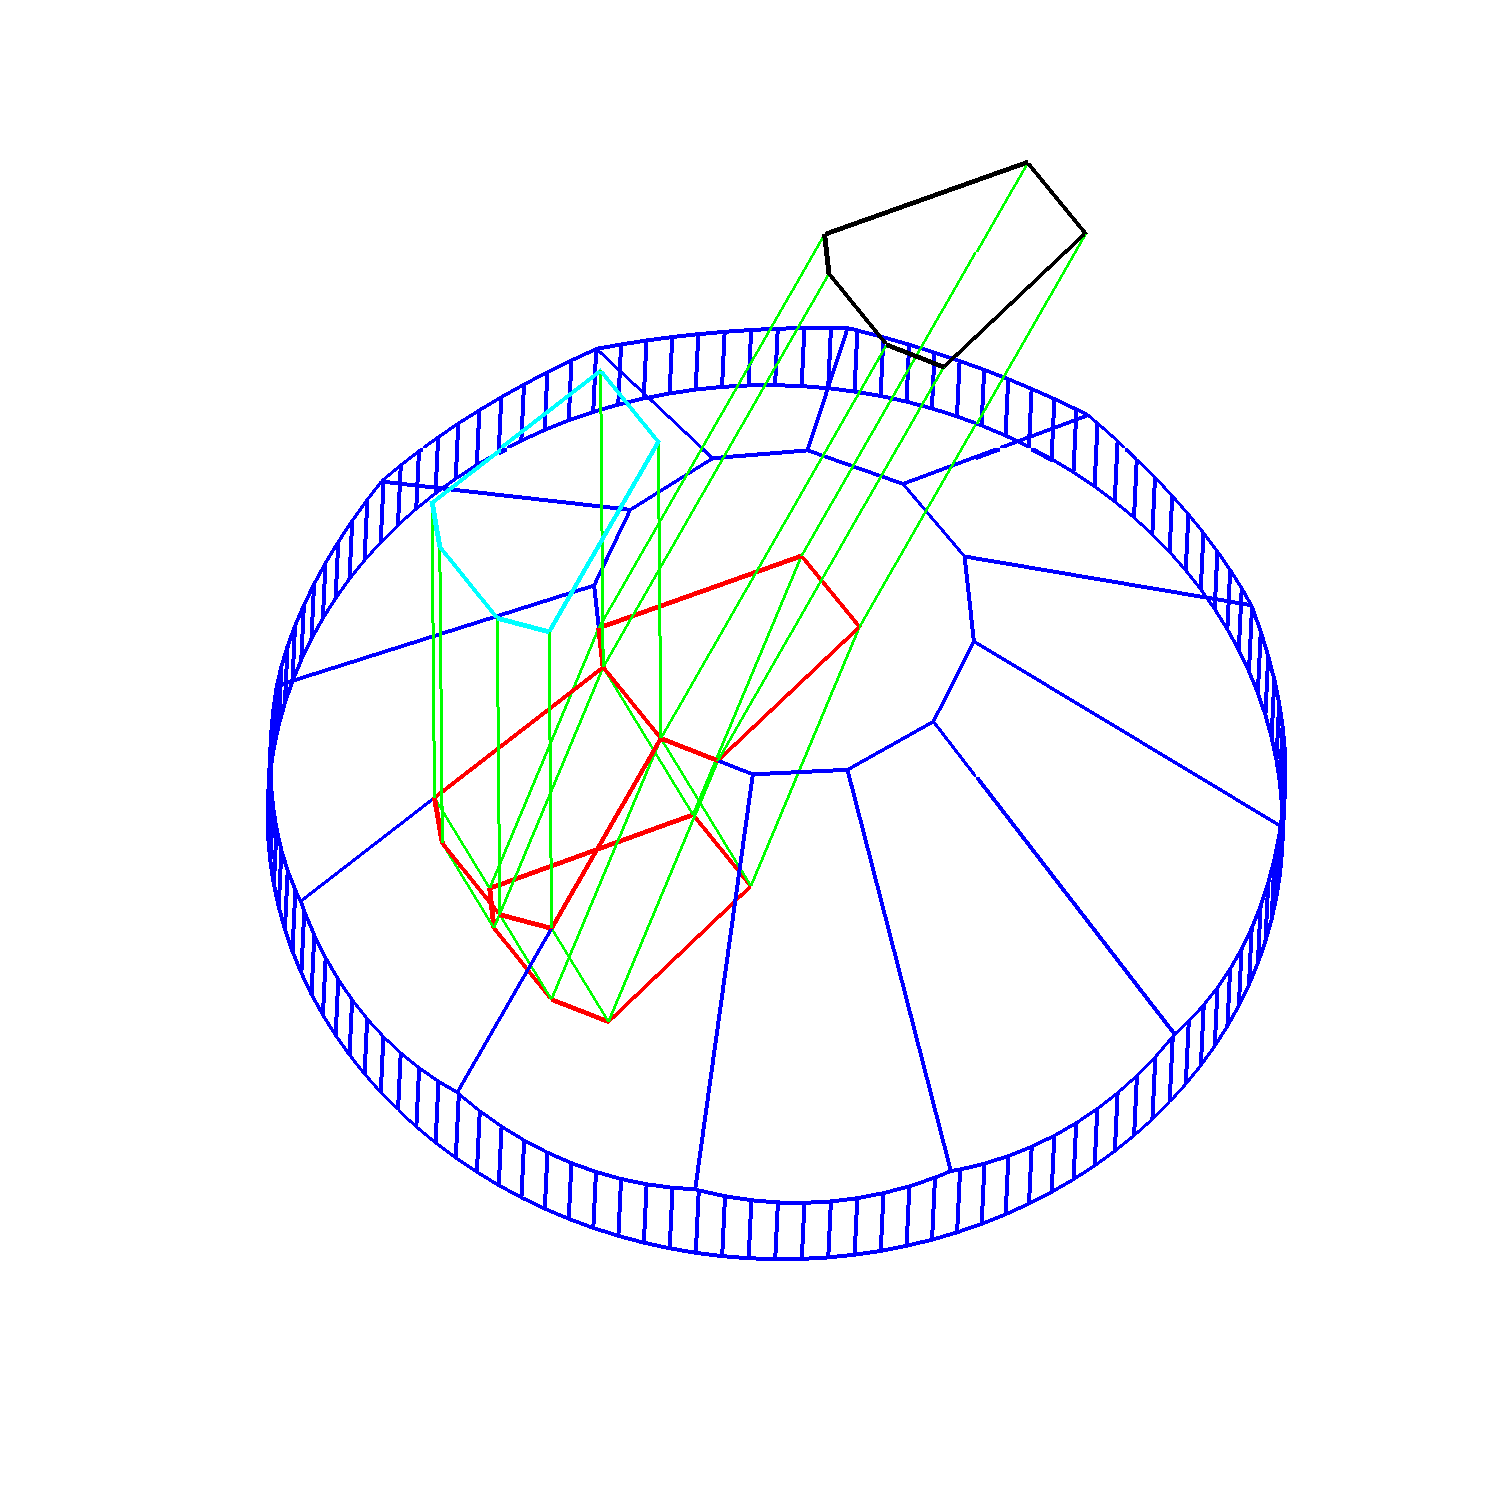
\includegraphics[width=\textwidth]{group3A.pdf}
\end{minipage}\\

\begin{minipage}[c]{0.325\textwidth}
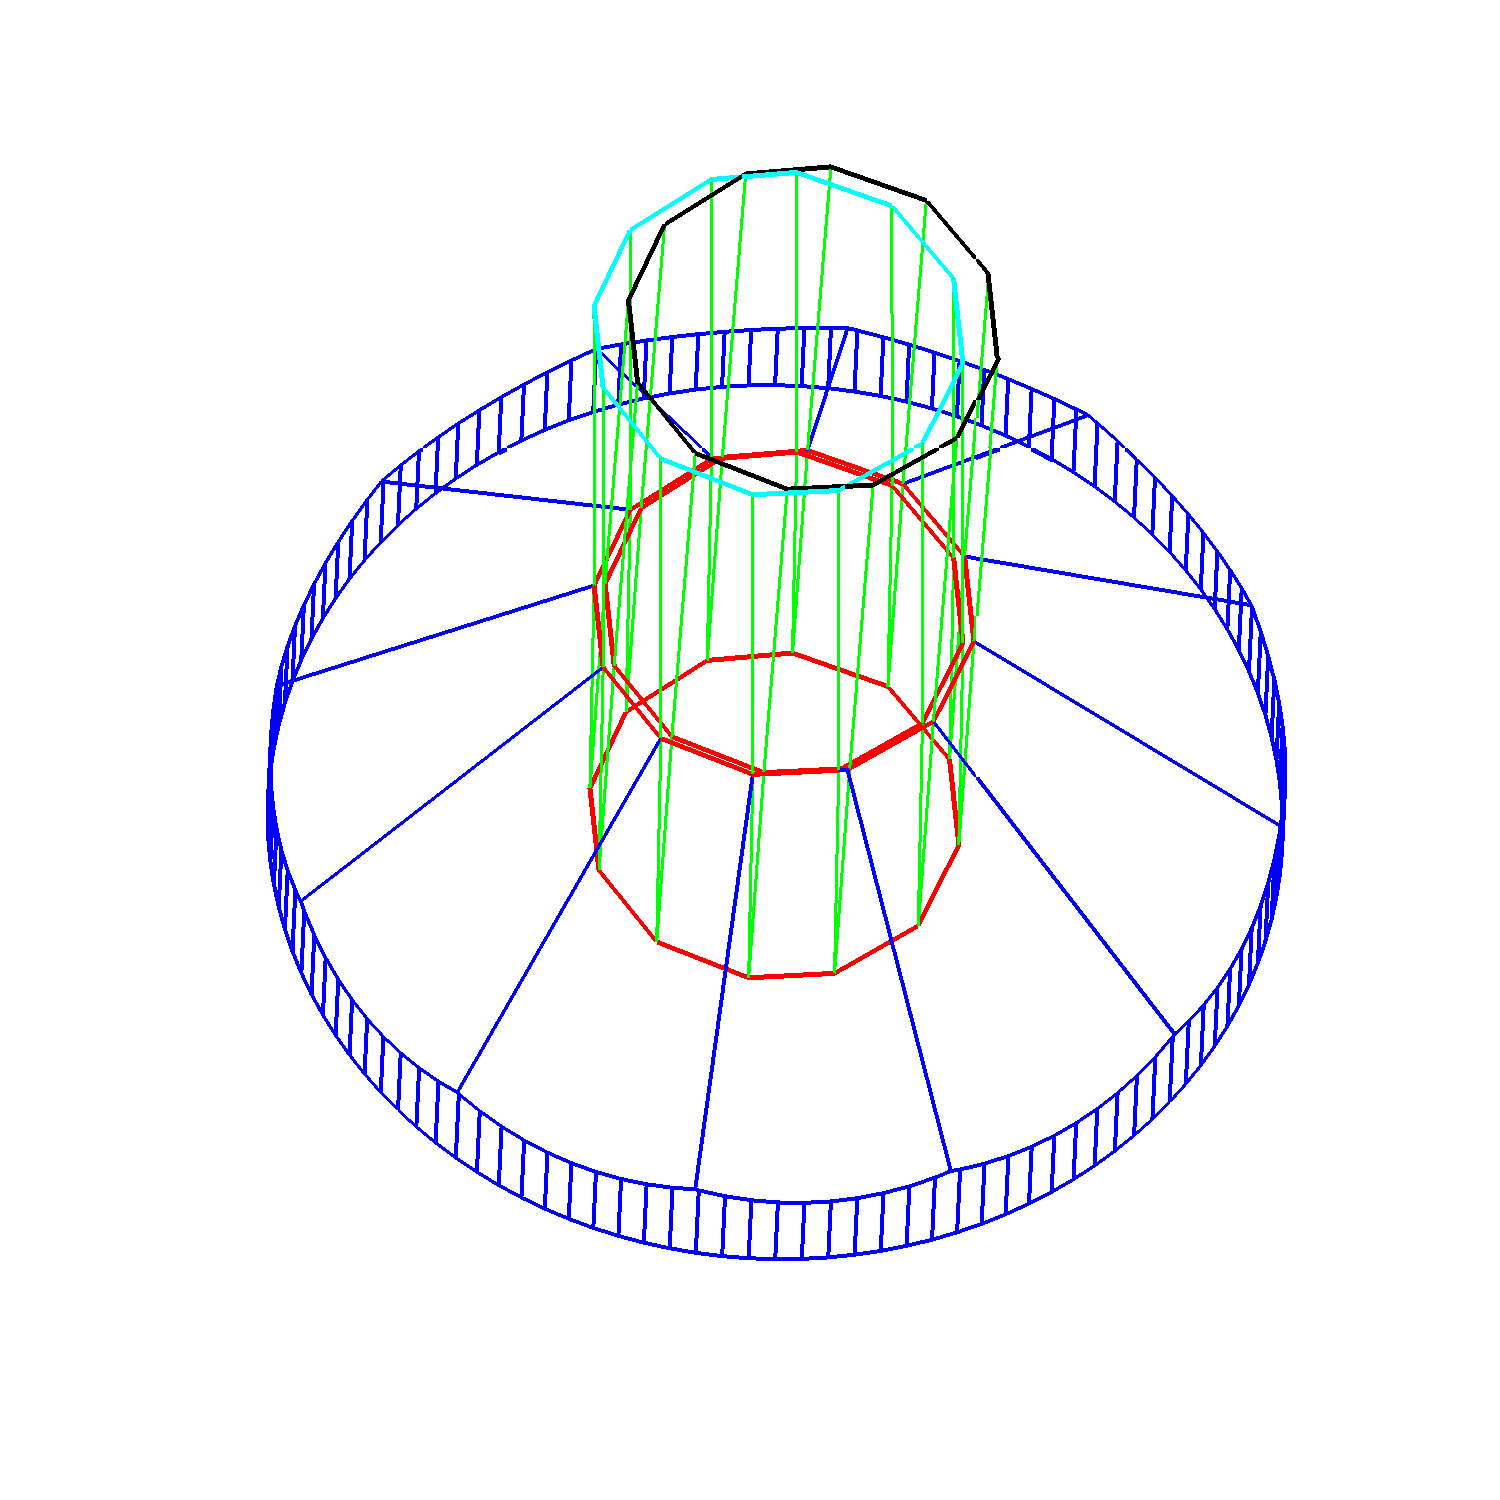
\includegraphics[width=\textwidth]{group3B.pdf}
\end{minipage}
\begin{minipage}[c]{0.325\textwidth}
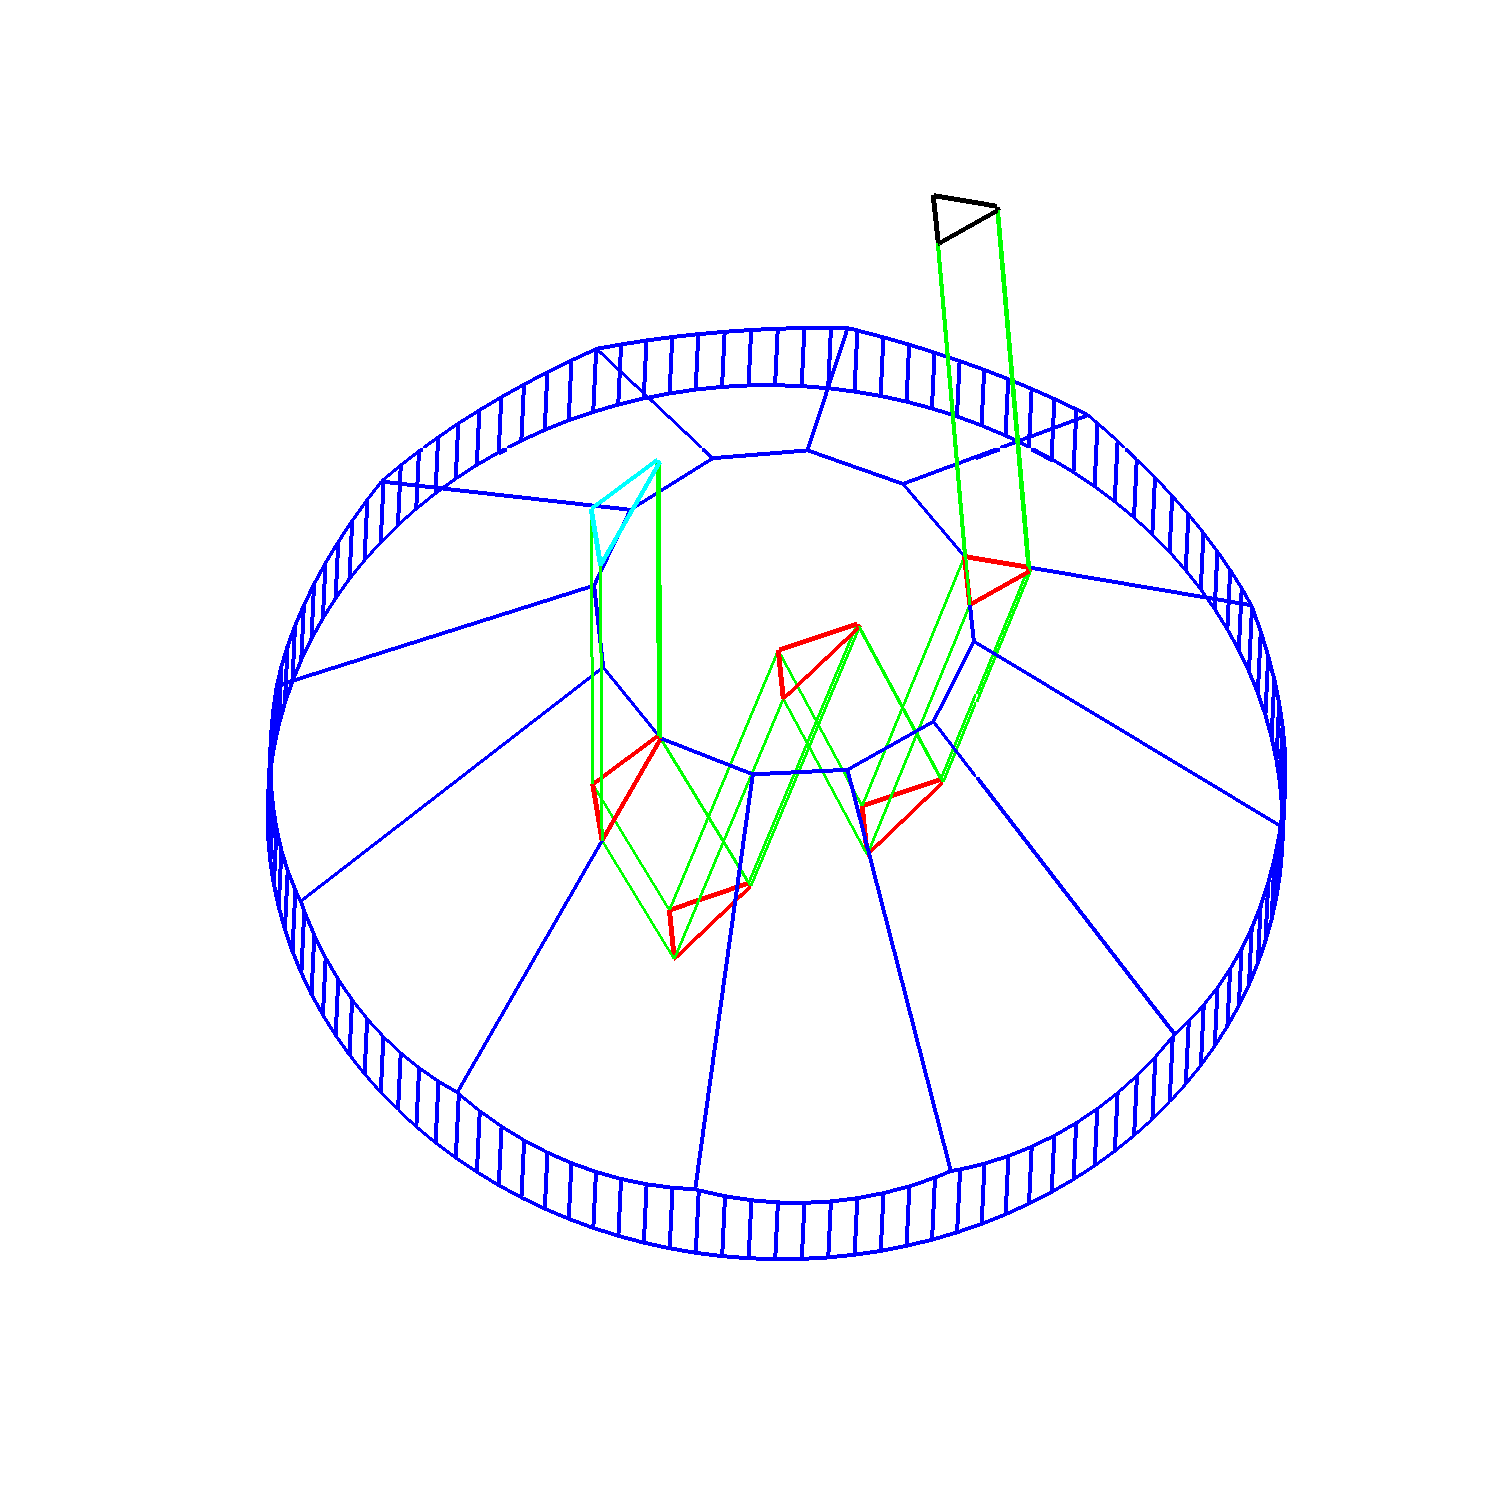
\includegraphics[width=\textwidth]{group5A.pdf}
\end{minipage}
\begin{minipage}[c]{0.325\textwidth}
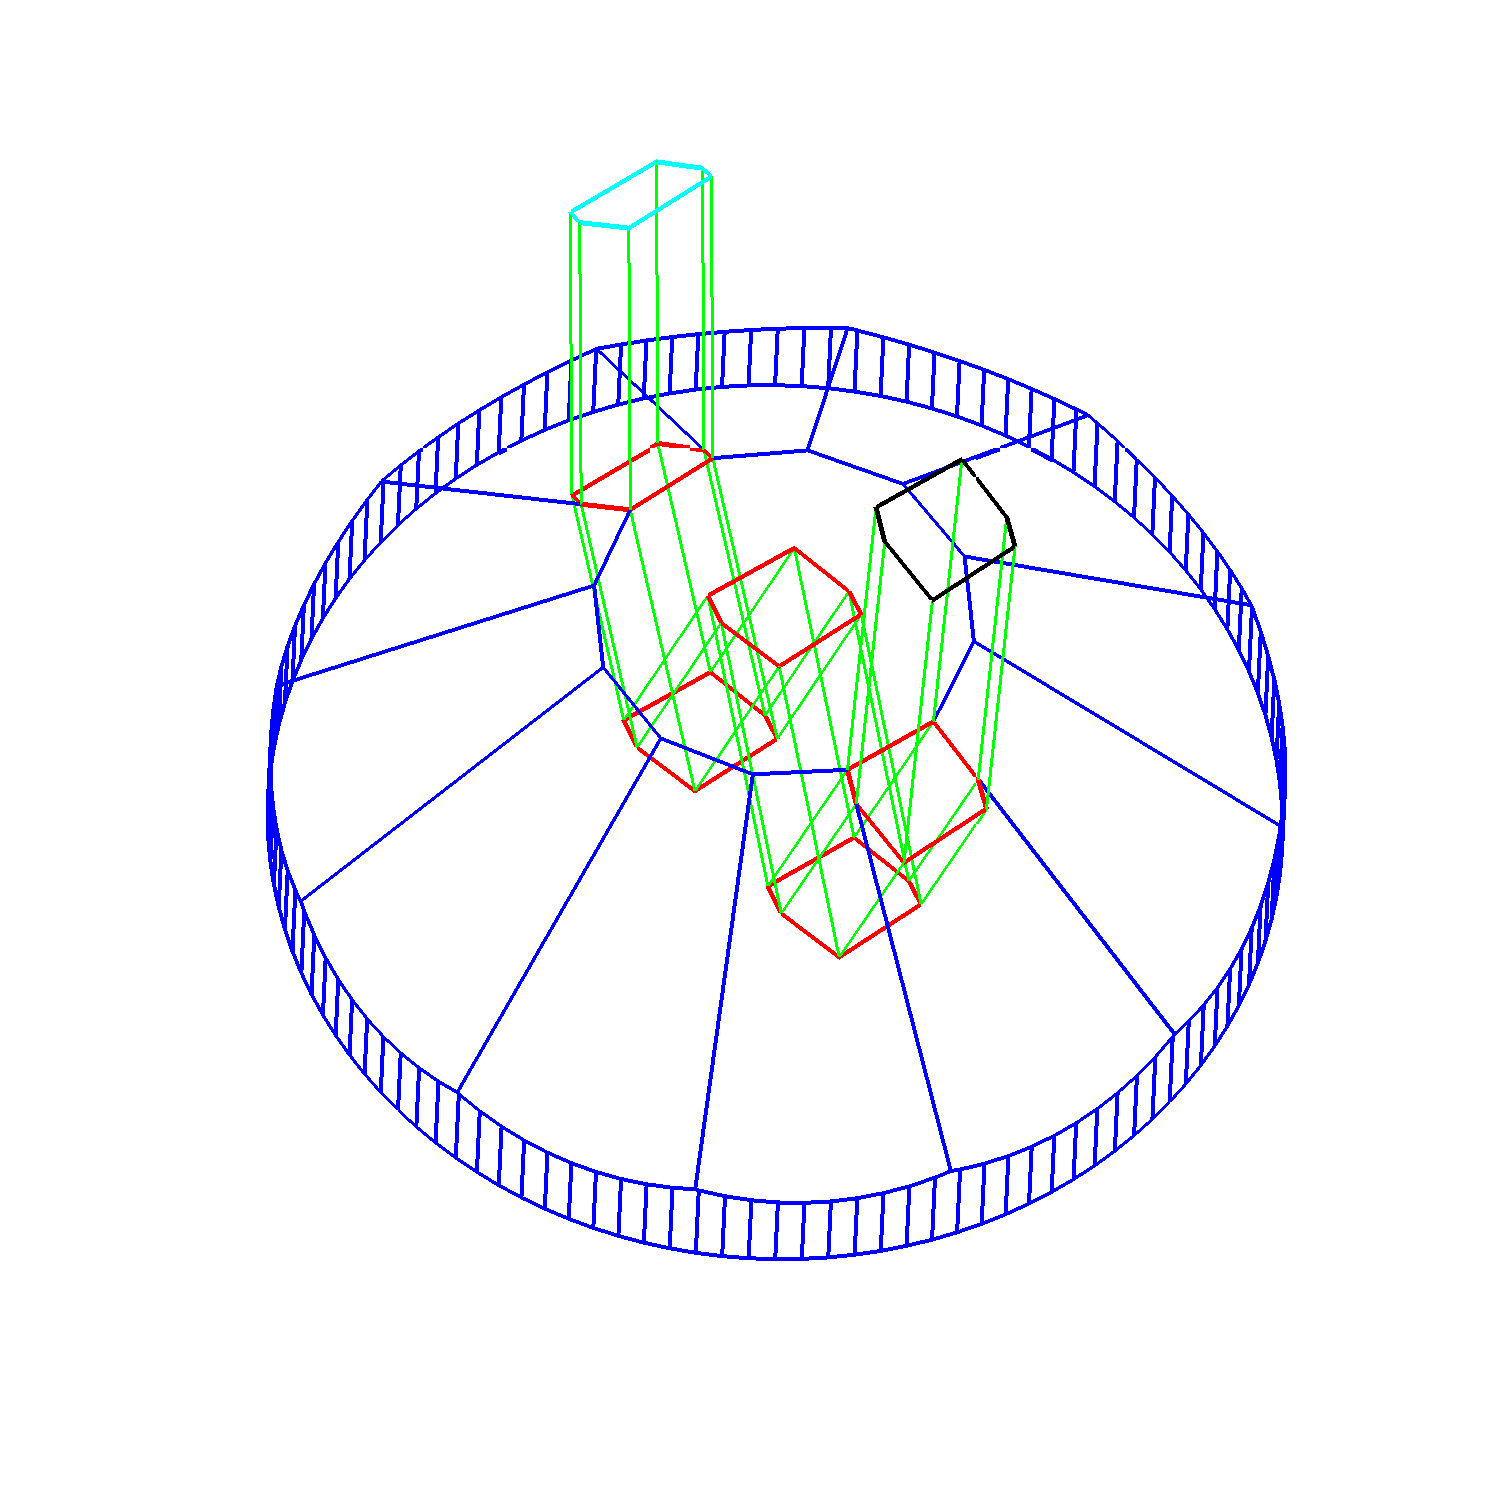
\includegraphics[width=\textwidth]{group5B.pdf}
\end{minipage}\\

\begin{minipage}[c]{0.325\textwidth}
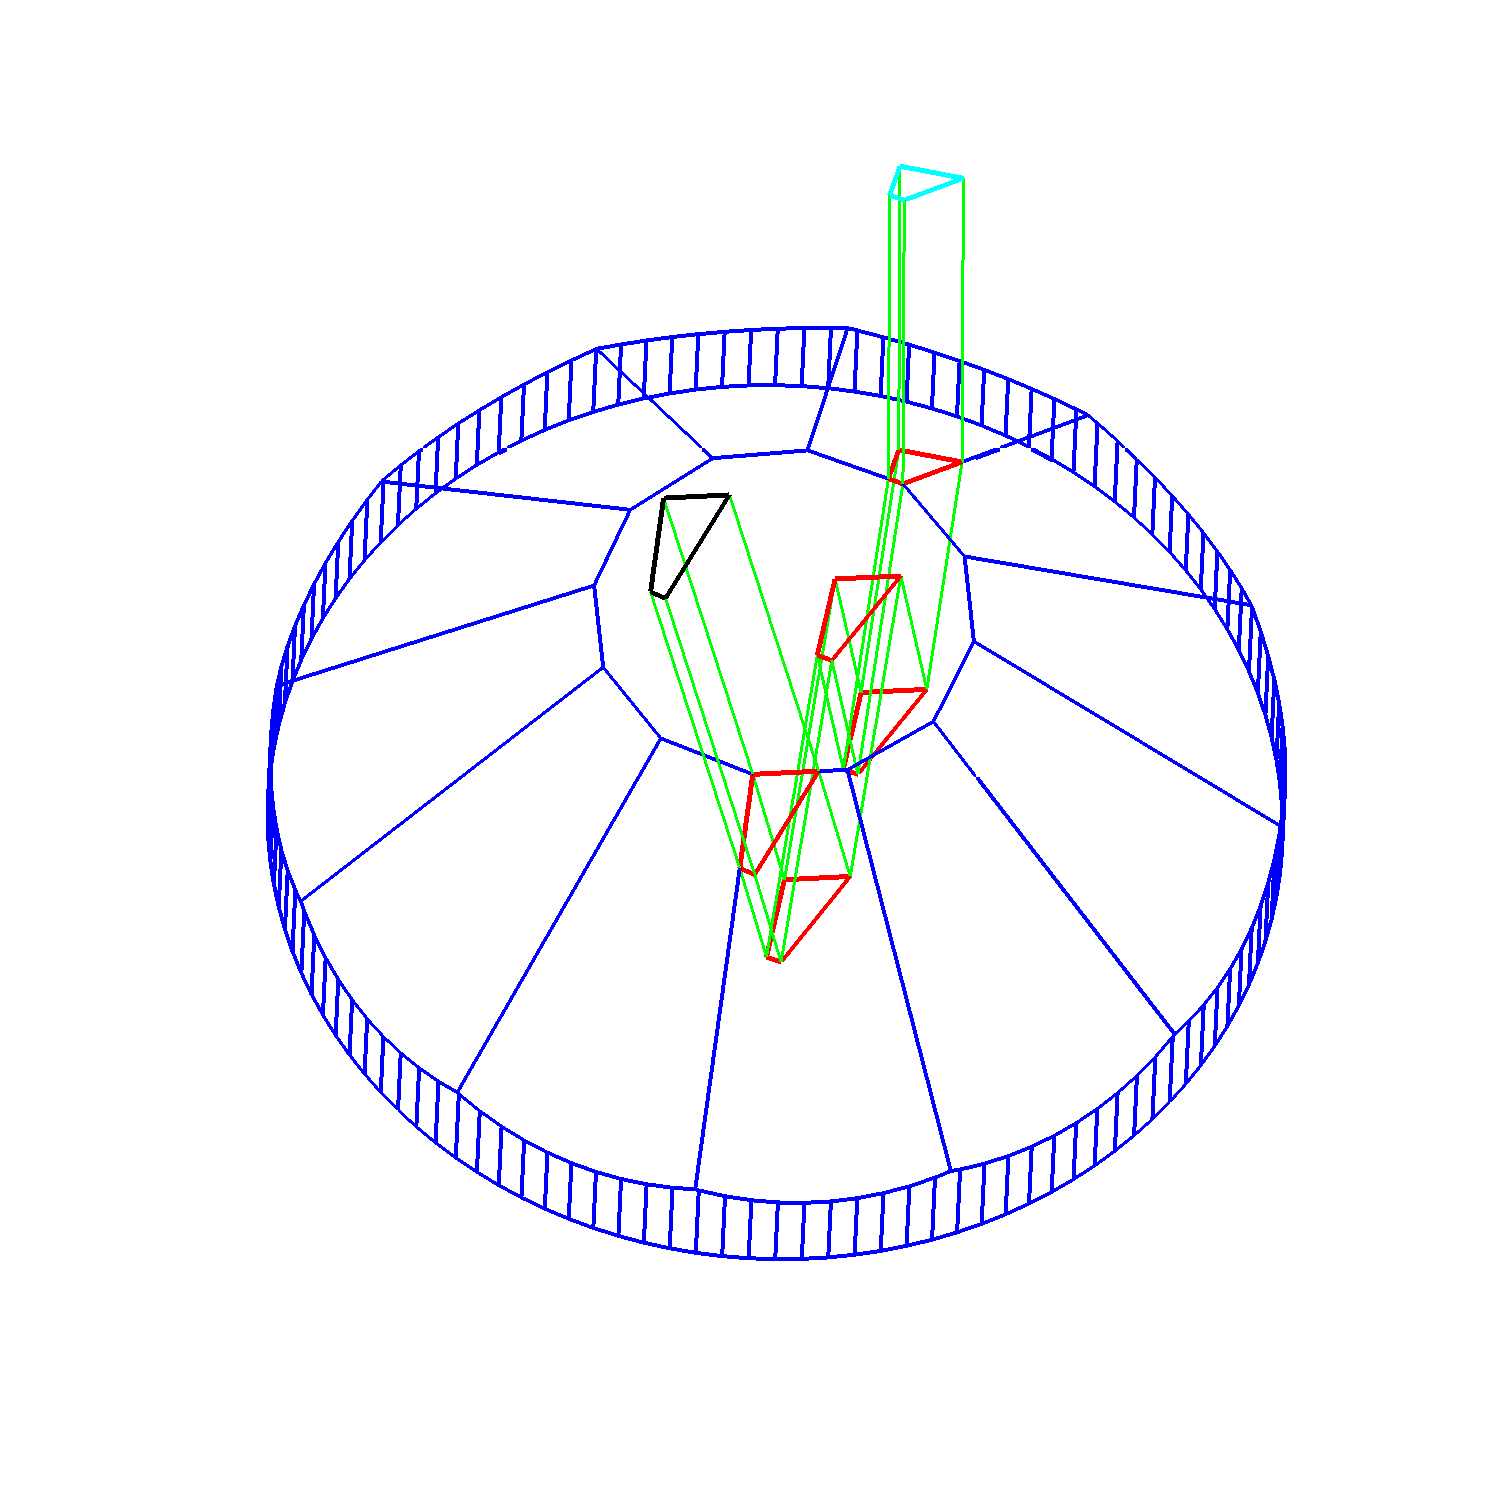
\includegraphics[width=\textwidth]{group5C.pdf}
\end{minipage}
\begin{minipage}[c]{0.325\textwidth}
\includegraphics[width=\textwidth]{group5D.pdf}
\end{minipage}
\begin{minipage}[c]{0.325\textwidth}
\includegraphics[width=\textwidth]{group5E.pdf}
\end{minipage}\\

\begin{minipage}[c]{0.325\textwidth}
\includegraphics[width=\textwidth]{group6A.pdf}
\end{minipage}
\begin{minipage}[c]{0.325\textwidth}
\includegraphics[width=\textwidth]{group6B.pdf}
\end{minipage}
\begin{minipage}[c]{0.325\textwidth}
\includegraphics[width=\textwidth]{group6C.pdf}
\end{minipage}

\caption{3D view of ray example in classes 1A, 1B, 3A, 3B, 5A, 5B, 5C, 5D, 5E, 6A and 6B.}
\label{fig:modelClass3D1}
\end{figure}



\begin{figure}[htps]
\centering
\begin{minipage}[c]{0.325\textwidth}
\includegraphics[width=\textwidth]{group6D.pdf}
\end{minipage}
\begin{minipage}[c]{0.325\textwidth}
\includegraphics[width=\textwidth]{group6E.pdf}
\end{minipage}
\begin{minipage}[c]{0.325\textwidth}
\includegraphics[width=\textwidth]{group6F.pdf}
\end{minipage}\\

\begin{minipage}[c]{0.325\textwidth}
\includegraphics[width=\textwidth]{group7A.pdf}
\end{minipage}
\begin{minipage}[c]{0.325\textwidth}
\includegraphics[width=\textwidth]{group7B.pdf}
\end{minipage}
\begin{minipage}[c]{0.325\textwidth}
\includegraphics[width=\textwidth]{group7C.pdf}
\end{minipage}\\

\begin{minipage}[c]{0.325\textwidth}
\includegraphics[width=\textwidth]{group7D.pdf}
\end{minipage}
\begin{minipage}[c]{0.325\textwidth}
\includegraphics[width=\textwidth]{group7E.pdf}
\end{minipage}
\begin{minipage}[c]{0.325\textwidth}
\includegraphics[width=\textwidth]{group7F.pdf}
\end{minipage}\\

\begin{minipage}[c]{0.325\textwidth}
\includegraphics[width=\textwidth]{group7G.pdf}
\end{minipage}
\begin{minipage}[c]{0.325\textwidth}
\includegraphics[width=\textwidth]{group7H.pdf}
\end{minipage}
\begin{minipage}[c]{0.325\textwidth}
\includegraphics[width=\textwidth]{group8A.pdf}
\end{minipage}

\caption{3D view of ray example in classes 6D, 6E, 6F, 7A, 7B, 7C, 7D, 7E, 7F, 7G, 7H, 8A.}
\label{fig:modelClass3D1}
\end{figure}


\begin{figure}[htps]
\centering
\begin{minipage}[c]{0.325\textwidth}
\includegraphics[width=\textwidth]{group8B.pdf}
\end{minipage}
\begin{minipage}[c]{0.325\textwidth}
\includegraphics[width=\textwidth]{group8C.pdf}
\end{minipage}
\begin{minipage}[c]{0.325\textwidth}
\includegraphics[width=\textwidth]{group8D.pdf}
\end{minipage}\\

\begin{minipage}[c]{0.325\textwidth}
\includegraphics[width=\textwidth]{group9A.pdf}
\end{minipage}
\begin{minipage}[c]{0.325\textwidth}
\includegraphics[width=\textwidth]{group9B.pdf}
\end{minipage}
\begin{minipage}[c]{0.325\textwidth}
\includegraphics[width=\textwidth]{group9C.pdf}
\end{minipage}\\

\begin{minipage}[c]{0.325\textwidth}
\includegraphics[width=\textwidth]{group9D.pdf}
\end{minipage}
\begin{minipage}[c]{0.325\textwidth}
\includegraphics[width=\textwidth]{group9E.pdf}
\end{minipage}
\begin{minipage}[c]{0.325\textwidth}
\includegraphics[width=\textwidth]{group9F.pdf}
\end{minipage}\\

\begin{minipage}[c]{0.325\textwidth}
\includegraphics[width=\textwidth]{group9G.pdf}
\end{minipage}
\begin{minipage}[c]{0.325\textwidth}
\includegraphics[width=\textwidth]{group9H.pdf}
\end{minipage}
\begin{minipage}[c]{0.325\textwidth}
\includegraphics[width=\textwidth]{group9I.pdf}
\end{minipage}

\caption{3D view of ray example in classes 8B, 8C, 8D, 9A, 9B, 9C, 9D, 9E, 9F, 9G, 9H, 9I.}
\label{fig:modelClass3D1}
\end{figure}









\part{Nový pozorovatelný příznak svazků}


%Cílem experimentu je objevit další parametr světelného svazku, jenž by v kombinaci s ostatními parametry pomohl rozpoznat měřené svazky. 

\section{Vzájemná rotace kamene a zdrojového svazku}
Pokusíme se nalézt směr či velikost rotace světelných svazků při rotaci kamene nebo při naklonění zdroje dopadajícího světelného svazku. 

Rotace kamene kolem osy způsobí změnu vlastností vystupujících světelných svazků (směru, zářivého toku, intenzity, vlastnosti ocásků atd.). Za určitých okolností může světelný svazek zcela vymizet. Tato situace nastává například při lomu světelného svazku z kamene do okolí. Když vlivem rotace překročíme kritický úhel, nedochází k lomu světelného svazku, ale k totálnímu odrazu na fasetě. Světelný svazek zanikne při posunu světelného svazku mimo fasetu, a to jak při odrazu, tak při lomu. Ze stejných důvodů, proč mohou světelné svazky vymizet, mohou naopak vzniknout svazky nové.

Uvažujeme zjednodušenou situaci, kdy světelný svazek nahradíme světelným paprskem ležícím v jeho pomyslném těžišti. 

Světelný paprsek necháme dopadat na zrcadlo pod úhlem $\varphi_1$. Paprsek se od zrcadla odráží podle známého zákonu odrazu pod úhlem $\varphi_1$. Při vychýlení světelného paprsku o úhel $ \delta $ v~ kladném směru úhlu $\varphi_1$ je odražený úhel $\varphi_1 + \delta$. Úhel odraženého paprsek se změní o úhel $ \delta $.

\begin{figure}[h!]
\begin{center}
\scalebox{1}{ \input{xfig/odraz2.pstex_t}}
\end{center}
\caption[Odraz světelného paprsku od zrcadla.]{Odraz světelného paprsku od zrcadla. Změna úhlu dopadajícího světelného paprsku vyvolá stejně velkou změnu úhlu odraženého paprsku.}
\label{fig:odraz laser}
\end{figure}

Jiná situace nastává při rotaci zrcadla kolem osy o úhel $\alpha$ v záporném směru. Světelný paprsek dopadá na zrcadlo pod úhlem $\varphi_1 + \alpha$ a  odráží se pod úhlem $\varphi_1+\alpha$. Úhel odraženého paprsku se v tomto případě změní o úhel $2\alpha$. 

Při rotaci kamene docílíme stejné změny odraženého paprsku jako při rotaci světelného zdroje o dvojnásobný úhel v opačném směru. Proto budeme dále uvažovat pouze rotaci kamene. 


\begin{figure}[h!]
\begin{center}
\scalebox{1}{ \input{xfig/odraz.pstex_t}}
\end{center}
\caption[Odraz světelného paprsku od rotujícího zrcadla.]{Odraz světelného paprsku od rotujícího zrcadla. Rotace zrcadla vyvolá dvojnásobnou změnu velikosti úhlu odraženého paprsku.}
\label{fig:odraz zrcadlo}
\end{figure}

\section{Změna směru vystupujících paprsků}
\label{sec: zmena smeru}
Pokud by docházelo pouze k odrazu od zrcadel v dvojrozměrné rovině, tak by naše zkoumání postrádalo smysl. Výstupní parsek by se vždy otočil o dvojnásobek úhlu rotace kamene, a to ve stejném směru. 

S uvažováním materiálu kamene s konstantním indexem lomu $ n_1~>~1 $ a okolí s indexem lomu $ n_2 = 1 $ se situace dramaticky mění. Vezměme si příklad lomu světelného paprsku z kamene přes rovinnou fasetu. Úhel dopadajícího paprsku na fasetu označme $\alpha_1$ a úhel lomeného svazku $\alpha_2$, pak můžeme podle Snellova zákona psát:

\begin{center}
$n_1\,\sin(\alpha_1) = n_2\,\sin(\alpha_2) = \sin(\alpha_2)\,.$
\end{center}

\begin{figure}[h!]
\begin{center}
\scalebox{.9}{ \input{xfig/index.pstex_t}}
\end{center}
\caption[Kritický úhel a totální odraz.]{Tři případy, které mohou nastat při dopadu světelného paprsku na fasetu. Zleva lom paprsku z kamene, dopad pod kritickým úhlem a totální odraz.}
\label{fig:lom ven }
\end{figure}

Zkoumejme změnu výstupního úhlu $\alpha_2$ na změně úhlu $\alpha_1$. Nejprve si vyjádříme úhel $\alpha_2$ následně zderivujeme podle $\alpha_1$. 
\begin{equation}
\alpha_2 = \arcsin(n_1\,\sin\alpha_1)
\label{eq:derivace uhlu1}  
\end{equation}
\begin{equation} \frac{\mathrm{d}\alpha_2}{\mathrm{d}\alpha_1}= \frac{n_1\,\cos\alpha_1}{\sqrt{1-n_1^2\,\sin^2\alpha_1}}
\label{eq:derivace uhlu}  
\end{equation}

Pokud se dostáváme ke kritickému úhlu ($\alpha_1 = \alpha_k$), dochází k totálnímu odrazu. 
\begin{equation}
 \sin\alpha_2 = 1 \implies \sin\alpha_1 = \frac{1}{n_1}
\end{equation}

Výpočtem limity rovnice \ref{eq:derivace uhlu} v okolí kritického úhlu pro $ n_1 > 1$ dostaneme 

\begin{eqnarray}
\lim_{\alpha_1 \to \alpha_k}\frac{\mathrm{d}\alpha_2}{\mathrm{d}\alpha_1} = \frac{n_1\,\cos(\arcsin\frac{1}{n_1})}{\sqrt{1-n_1^2\,\frac{1}{n_1^2}}} \to \infty\,.
\label{eq:zmena velikosti posunu}  
\end{eqnarray},

Z grafu \ref{fig:derivace uhlu} zjistíme, že minimum funkce $\frac{\mathrm{d}\alpha_2}{\mathrm{d}\alpha_1}$ vychází pro $ \alpha_1 = 0^\circ $. Po dosazení
\begin{eqnarray}
{\frac{\mathrm{d}\alpha_2}{\mathrm{d}\alpha_1}}\biggr\rvert_{\alpha_1 = 0^\circ}= \frac{n_1}{\sqrt{1-0}} = n_1\,.
\end{eqnarray}


Velikost změny posunu světelného svazku tedy může být teoreticky libovolně větší než je index lomu $n_1$. 

\begin{figure}[h!]
\begin{center}
\includegraphics[width = 0.8\linewidth]{derivace.pdf}
\end{center}
\caption[Závislost změny lomeného úhlu na změně úhlu dopadu.]{Závislost změny lomeného úhlu na změně úhlu dopadu. Pro kritický úhel $\alpha_k$ roste k~nekonečnu. Graf funkce popsané vzorcem \ref{eq:zmena velikosti posunu}.}
\label{fig:derivace uhlu}
\end{figure}



\section{Modelování pohybu svazků}
V programu LADOK jsme provedli experiment s rotací broušeného kamene \textit{viva12}.

Rotací kamene okolo osy kolmé ke spodku kamene dostaneme pouze soustředné kružnice. Kámen jsme tedy rotovali kolem vodorovné osy procházející středem spodku kamene o konstantní úhel v každém kroku. Zaznamenali jsme směry vystupujících svazků při různých pozicích kamene. Výsledek jsme vykreslili do polárního grafu. Ze dvou po sobě následujících pozic kamene jsme šipkou spojili pozici svazků se stejným seznamem dopadových faset. Výsledný obrazec je znázorněn na obr. \ref{fig:relativni pohyb graf}.

Z praktického hlediska nás mohou zajímat pouze svazky, které vytvoří po dopadu na stínítko detekovatelnou stoupu.

% obrazek pohybu jednotlivych stop 
\begin{figure}[h!]
\begin{center}
   \begin{minipage}[c]{0.48\textwidth}
     \centering \includegraphics[width = 1\linewidth]{viva12_bigflux.eps}
   \end{minipage}
   \begin{minipage}[c]{0.48\textwidth}
     \centering \includegraphics[width = 1\linewidth]{viva12_bigflux2.eps}
   \end{minipage}
 \end{center}
\caption[Dráhy pohybu svazků při rotaci kamene.]{Dráhy směru svazků vycházejících z kamene \textit{viva12} získané pomocí simulačního programu  LADOK při rotaci kamene. Zobrazeny jsou pouze svazky s významným zářivým tokem vycházející v horního poloprostoru kamene. Vpravo detail na střed obrázku vlevo.}

\label{fig:relativni pohyb graf}
\end{figure}

Pro lepší představu o změně směru jednotlivých svazků nám může být užitečný kruhový histogram znázorňující směr jejich pohybu (obr. \ref{fig:relativni pohyb graf}). Podstatná většina svazků se posouvá ve směru rotace kamene, což není příliš nápomocné při jejich identifikaci.

Existují však svazky, které jsou svým pohybem charakteristické a lze je tedy oddělit od ostatních. Kritérium pro rozpoznání svazků nemusí být pouze směr pohybu, ale jak vidíme na obr. \ref{fig:relativni pohyb graf} i velikost úhlu rotace. V neposlední řadě přichází v úvahu i změna zářivého toku svazků, změna velikosti ocásků a další. 

\begin{figure}[h!]
 \begin{center}
   \begin{minipage}[c]{0.48\textwidth}
     \centering \includegraphics[width = \linewidth]{relative.eps} 
   \end{minipage}
   \begin{minipage}[c]{0.48\textwidth}
     \centering \includegraphics[width =\linewidth]{relative_index1.eps} 
   \end{minipage}
 \end{center}
\caption[Histogram velikosti rotace vystupujících svazků.]{Vlevo: histogram velikosti úhlu rotace vystupujících svazků z kamene \textit{viva12} z obrázku \ref{fig:relativni pohyb graf}. Vlivem lomu je relativní rotace v mnoha případech větší než 2. V okolí kritického úhlu roste k~nekonečnu. Pokud ztotožníme indexy lomu kamene a okolí, tak relativní rotace nebude větší než 2. To lze vidět na histogramu vpravo.}

\label{fig:histogram relativni pohyb }

\end{figure}

Vykresleme si histogram (obr. \ref{fig:histogram relativni pohyb } vlevo) relativní velikosti úhlu rotace vystupujících svazků. Z něj je patrné, že řada svazků rotuje o více než dvojnásobek úhlu rotace kamene $\alpha$, což potvrzuje teorii o relativní změně směru svazků z rovnice \ref{eq:zmena velikosti posunu}. 



\begin{figure}[h!]
\begin{center}
\includegraphics[width =0.7\linewidth]{kruhovy_histogram.eps}
\end{center}
\caption[Kruhový histogram směru rotace svazků - \textit{viva12}.]{Kruhový histogram směru rotace vystupujících svazků kamene \textit{viva12} z obrázku \ref{fig:relativni pohyb graf}. Většina svazků se pohybuje ve směru rotace kamene.}
\label{fig:kruhovy histogram}
\end{figure}

Pokud vezmeme kámen o stejném indexu lomu, jako je okolí, nedochází k lomu. Potom by se nemělo docházet k rotaci výstupního svazku o úhel větší než $2\alpha$, způsobená právě rozdílným indexem lomu. Pro potvrzení této teorie jsme provedli stejnou simulaci jako v~předchozím případě. Indexy lomu kamene a jeho okolí jsme ztotožnili a výsledek simulace ukázal, že rotace výstupních svazků úhel větší než $2\alpha$ se již nevyskytují. To nám dokládá zhotovený histogram (obr. \ref{fig:histogram relativni pohyb } vpravo).


Téměř konstantní směrovost rotace svazků u kamene \textit{viva12} zmenšuje význam příspěvku této vlastnosti k lepšímu rozpoznání světelných stop. Pokud ovšem provedeme stejný experiment na broušeném kameni jiného tvaru, dostaneme rozdílný výsledek. Například u šatonu, svým tvarem složitějším než \textit{viva12}, je směr rotace svazků rozmanitější. Velká část z nich samozřejmě rotuje ve směru rotace kamene. Jak ale vidíme z kruhového histogramu (obr. \ref{fig:kruhovy histogram saton}), lze rozlišovat i velké množství stop pohybujících se např. pod úhlem $45^\circ$. U šatonu tedy může znalost směru pohybu svazků při rotaci kamene nemalou měrou pomoci v jejich rozpoznání. 

\begin{figure}
\begin{center}
\includegraphics[width = 0.7\textwidth]{saton_smer.eps}
\end{center}
\caption[Kruhový histogram směru rotace svazků - šaton.]{Kruhový histogram směru rotace vystupujících svazků z šatonu při rotaci kamene.}

\label{fig:kruhovy histogram saton}
\end{figure}

  
\clearpage
\part{Terminologie}

Je důležité rozlišit svazky získané pomocí simulace v LADOKu a svazky získané experimentálním měřením.   
Proto zavedeme \textit{simulované} a \textit{měřené} svazky.

\section{Simulované svazky}
\begin{enumerate}

\item 	Získáme potřebné parametry kamene, který zkoumáme. Zdrojem může být technický výkres, nebo předchozí měření.  

\item	Sestavíme model, který bude přibližně určovat tvar kamene. Tento model budeme považovat za \textit{referenční}.

\item	V programu LADOK simulujeme průlet svazku \textit{referenčním} modelem. Pro simulaci je důležité znát elektromagnetické vlastnosti laserového svazku a index lomu kamene. 

\item	Výsledkem simulace jsou parametry \textit{simulovaných} svazků.

\end{enumerate}

\section{Měřené svazky}
Předpokladem pro získání parametrů měřených svazků je sestavení a kalibrace měřicí soustavy podle \cite{Drapela}. % odkay na kapitolu
\begin{enumerate}

\item 	Opracovaný kámen umístíme do měřicí soustavy.

\item	Provedeme experiment průchodu svazku kamenem podobný situaci v simulačním programu LADOK. 

\item	Získáme obraz dopadu svazků na stínítko. 

\item	V obraze detekujeme světelné stopy (kapitola \ref{sec:detection}).  

\item	Z detekovaných stop vypočítáme parametry \textit{měřených} svazků (kapitola \ref{sec:beam parameters}).

\end{enumerate}

\clearpage
%Přecházíme k situaci, kdy máme dostupné informace o \textit{simulovaných} i \textit{reálných} svazcích. Mezi těmito dvěma množinami je třeba nalézt korespondence. Korespondující svazky si odpovídají seznamem faset kamene, na které při své cestě dopadají.  
%
%Pro korespondující páry určíme chybovou funkci a parametry budeme optimalizovat. Optimalizační algoritmus odhadne takové nastavení parametrů, aby bylo optimalizované kritérium co nejmenší. 
%
%Optimalizované parametry použijeme k výpočtu \textit{optimalizovaného} modelu kamene. Orientace faset broušeného kamene odečteme z \textit{optimalizovaného} modelu.   
\part{Optimalizace orientace faset}
	
\section{Schéma optimalizačního procesu}

%Přecházíme k situaci, kdy máme dostupné informace o \textit{simulovaných} i \textit{reálných} svazcích. Mezi těmito dvěma množinami je třeba nalézt korespondence. Korespondující svazky si odpovídají seznamem faset kamene, na které při své cestě dopadají.  
%
%Pro korespondující páry určíme chybovou funkci a parametry budeme optimalizovat. Optimalizační algoritmus odhadne takové nastavení parametrů, aby bylo optimalizované kritérium co nejmenší. 
%
%Optimalizované parametry použijeme k výpočtu \textit{optimalizovaného} modelu kamene. Orientace faset broušeného kamene odečteme z \textit{optimalizovaného} modelu.   

% diagram je vytvoren -> 500pm -> bitmap -> online to EPS -> latex to PDF -> load PDF
\begin{figure} [h!]
\centering
\includegraphics[width = 0.8\textwidth]{diagram.pdf}
\caption{Diagram s principem odhadu orientace faset broušených kamenů.}
\label{fig:diagram}
\end{figure}

\clearpage


\section{Optimalizované kritérium}
\label{sec:Optimalizace_crit}
Optimalizační algoritmus je převzat z práce \cite{Bodlak2005}. Některé části byly pozměněny. Ukážeme si stručný přehled metody optimalizace a zvýrazníme provedené úpravy. Optimalizační algoritmus používáme nejen k odhadu parametrů faset kamene, ale také k odhadu indexu lomu kamene a jeho orientace kamene v měřené soustavě.

Definujeme kriteriální funkci, kterou budeme optimalizovat. Funkci lze popsat vztahem 

\begin{equation}
\vec{\varepsilon} = h\left(\vec{x},\vec{v},\vec{l},\vec{p} \right)\,,
\label{eq: opt_criter}
\end{equation}

\begin{tabular}{l p{12cm}}
$\vec{p}$ & Obsahuje směrové vektory \textit{reálných} svazků. Směr popisujeme pomocí souřadnic azimutu a elevace. Pokud pro výpočet optimalizačního kritéria použijeme $s$ \textit{reálných} svazků, bude mít vektor $\vec{p}$ délku $2\,s$. \\ & \\

$\vec{l}$ & Obsahuje seznam dopadových faset svazku. Tento seznam je využit pro výpočet směru výstupního svazku. Délka seznamu se musí rovnat $s$. \\ & \\

$\vec{v}$ & Popisuje směr zdrojového svazku světla\\ & \\  

$\vec{x}$ & Vektor parametrů, které nastavuje optimalizační algoritmus.
\paragraph{Parametry faset, index lomu}

 Jedná se převážně o parametry $r$ uvolněných faset. Každou fasetu lze parametrizovat pomocí úhlové změny normálového vektoru $\vec{n}$ (2 parametry) a změny vzdálenosti $d$ fasety od souřadného systému (1 parametr).\\
& Optimalizační metoda nemá dostatečnou citlivost na změny vzdálenosti $d$ fasety \cite{Bodlak2005}. Tento parametr proto považujeme za konstantu.\\
& Nově lze mezi optimalizované parametry přidat index lomu kamene $n_i$. Celkově máme $2\,r + q$ parametrů, kde $q$ je 1 pokud je mezi $\vec{x}$ parametr $n_i$, jinak je $q$ rovno 0.

\paragraph{Orientace} Orientaci kamene popisujeme rotací kolem vertikální osy $R_z$ a dvou parametrů definujících náklon kamene $R_x$, $R_y$. 
 \\ & \\

$\vec{\varepsilon}$ & Představuje vektor odchylek v elevaci a azimutu \textit{simulovaných} a \textit{reálných} svazků.\\ 
& V práci \cite{Bodlak2005} byla tato odchylka měřena jako chyba v pozici dopadu laserového svazku na stínítku. Důvodem proč bylo využíváno toto kritérium byla citlivější odezva při změně vektoru svazku. Hlavním důvodem volby azimutu a elevace pro výpočet optimalizačního kritéria je vyšší rychlost. Odpadá totiž potřebný výpočet, který transformuje směrový vektor do souřadnic na stínítku.\\ & Vektor $\vec{\varepsilon}$ má $2\,s$ prvků.\\ & \\

\end{tabular}


\section{Plná vs. zjednodušená simulace}
V optimalizačním cyklu je použito dvou simulací, které simulují průlet světla broušeným kamenem.

\subsection{Plná simulace}
Plnou simulací rozumíme klasický program LADOK, který modeluje odraz a lom svazků v konvexním tělese. Nevýhodou algoritmu je ale to, že simulace trvá příliš dlouho na to, aby mohla být úspěšně použita v optimalizačním procesu.

\subsubsection{Časová náročnost simulace v LADOKu}
	U matematická simulace programu LADOK můžeme nastavit do jaké hloubky budou simulovány měřené svazky. Při řešení se můžeme omezit svazky s maximálním počtem dopadových faset $n_d$. V grafu \ref{fig: ladok_time} je zakreslena časová závislost programu LADOK při výpočtu referenčních svazků kamene \textit{viva12} po různý počet dopadových faset. 
	
	\begin{figure}[htbp]
    \centering\includegraphics[width=0.7\textwidth]{ladok_time.eps}
     \caption[Časová náročnost simulace - LADOK.]{Výpočetní doba simulace referenčních svazků v programu LADOK v závislosti na počtu dopadových faset svazků.}
 \label{fig: ladok_time}
 \end{figure}

	
	Vzhledem ke strmému nárůstu časové náročnosti simulace programu LADOK budeme před každým výpočtem volit minimální $n_d$, tak abychom získali informace o všech referenčních svazcích, které v dané situaci potřebujeme.      


\subsection{Zjednodušená simulace}
Základní myšlenkou je, že se optimalizované parametry $\vec{x}$ příliš nemění. Za tohoto předpokladu si podstatná část svazků zachová posloupnost dopadových faset. Vynecháme proto kontrolu vzniku či zániku svazků. 

Zjednodušená simulace vyřadí z plné simulace zbytečné výpočty, které v procesu optimalizace nevyžíváme. 
Jediné, co potřebujeme znát je směr výstupních svazků. Pro výpočet směru nahradíme svazky nekonečně tenkými paprsky a můžeme s nimi pracovat jako s vektory. Fasety kamene reprezentujeme pomocí normálového vektoru. 

Zjednodušená simulace přistupuje k paprsku jednotlivě. Funkci pro výpočet vektoru výstupního paprsku $\vec{v_o}$ lze vyjádřit jako  

\begin{equation}
\vec{v_o}= g\left(\vec{v_i},\vec{N} \right)\,,
\end{equation}
kde $\vec{v_i}$ je vektor vstupního paprsku. Vektor $\vec{N}$ obsahuje normály $\vec{n_1},\dots,\vec{n_m}$ faset na které svazek dopadá. Normály jsou seřazené v pořadí odpovídající dopadovým fasetám při šíření paprsku od zdroje ke stínítku. 

Při výpočtu musíme vědět, která faseta svazek odráží a která lomí. Situace je jednoduchá. Pokud $m = 1$, potom muselo dojít k odrazu. Pokud  $m > 1$  odpovídají normály $\vec{n_1}$ a $\vec{n_m}$ fasetám, přes které se svazek lomí. Na ostatních fasetách se svazek odrazí. 

Zjednodušená simulace v LAMu navíc počítá polohu, kam paprsek na fasetu dopadl. Výpočet polohy byl z důvodu rychlosti výpočtu odstraněn.



\section{Podmíněnost}
Základní otázkou optimalizačního problému je, zda je systém dostatečně podmíněný. První podmínku, kterou musíme splnit je získat minimálně stejný počet nezávislých rovnic, jako je počet optimalizovaných parametrů. 

V optimalizačním kritériu máme celkem  $2\,r + q$ nezávislých rovnic. Základní podmínkou je, že počet korespondencí musí být minimálně $ s+q $.

\subsection{Třída svazků \textbf{1A} a \textbf{1B}}
Od tříd \textbf{1A} a \textbf{1B} lze obecně čekat velmi dobrou podmíněnost. Jednotlivý svazek z těchto tříd dopadne pouze na jednu fasetu a směr odraženého svazku jednoznačně určuje parametry fasety, od které se svazek odrazil. Pokud by máš matematický model přesně odpovídal reálnému experimentu, potom postačí nalézt korespondence třídy \textbf{1A} \textbf{1B}, abychom určili parametry všech faset kromě spodku. Tyto třídy nepodmiňují index lomu kamene.
 
\subsection{Třída \textbf{3A}}
Teoreticky korespondencí svazků třídy \textbf{3A} (např. UF1-TOP-BOT) získáme 2 rovnice $\Delta e$ a $\Delta \alpha$, které jsou závislé na parametrech dopadových faset UF1, TOP a BOT. Problém spočívá v tom, že tato korespondence určuje pouze vzájemnou polohu dopadových faset a nelze u této třídy očekávat dobrou podmíněnost. 
Abychom mohli optimalizovat náklon faset, potřebujeme znát další třídy korespondencí.  

\section{Pozorování}

\subsection{Vzájemná poloha svazků}

Simulujeme průlet světelného svazku optickým klínem (obr. \ref{fig:wedge}). Prostředí s indexy lomu $\eta_1$, $\eta_2$ a $\eta_3$ oddělují rozhraní $\rho_1$ a $\rho_2$. Tyto rozhraní mezi sebou svírají úhel $\alpha$.
\begin{figure}[h!]
\begin{center}
\scalebox{0.8}{ \input{xfig/mirror2.pstex_t}}
\end{center}
\caption{Lom a odraz paprsku v optickém klínu.}
\label{fig:wedge}
\end{figure}

\begin{equation}
\gamma = \arcsin{\left(\frac{\eta_1}{\eta_2}\sin{\beta}\right)}\,.
\end{equation}

\begin{equation}
\varepsilon_1 = \arcsin{\left(\frac{\eta_2}{\eta_1}\sin{\left(\gamma + 2\,\alpha\right)}\right)}\, 
\rightarrow \begin{cases}
\alpha > 0, & \varepsilon_3 > \varepsilon_2 > \varepsilon_1 > \beta\\
\alpha = 0, & \varepsilon_3 = \varepsilon_2 = \varepsilon_1 = \beta\\
\alpha > 0, & \varepsilon_3 < \varepsilon_2 < \varepsilon_1 < \beta
\end{cases}
\end{equation}


Svazek dopadá na rozhraní $\rho_1$ pod úhlem $\beta$. Na obrázku \ref{fig:wedge} je tento svazek reprezentován paprsek č.0. 

Svazek světla můžeme charakterizovat velikostí zářivého toku $\phi_e$. Z Fresnelových rovnic víme, že pokud na rozhraní $\rho_1$ nedochází k totálnímu odrazu, tak po dopadu svazku na rozhraní vznikne odražený a lomený svazek. Jaká bude velikost zářivého toku odraženého svazku $\phi_{e_{reflect}}$ závisí na polarizaci světla, dopadajícím úhlu a poměrem mezi indexy lomu prostředí, které odděluje rozhraní $\rho_1$.

\begin{equation}
\phi_e = \phi_{e_{reflect}} + \phi_{e_{refract}}\,.
\end{equation}

 Při dopadajícím úhlu $\beta = 0^\circ$ a indexech lomu $\eta_1 = 1$, $\eta_2 = 1.5$ se \SI{4}{\percent} dopadajícího zářivého toku odrazí. $\frac{\phi_{e_{reflect}}}{\phi_e} = 0.04$, $\frac{\phi_{e_{refract}}}{\phi_e} = 0.96$.

Z principu šíření světla optickým prostředím pozorujeme svazky 0 až 9, se specifickým směrem šíření. 

V šatonové růži nastává stejný optický jev mezi tabulkou (TOP) a spodkem (BOT), kde
\vspace{4mm}
\begin{tabular}{p{2cm} l}
$\eta_1$ & index lomu vzduchu,\\
$\eta_2$ & index lomu materiálu kamene,\\
$\eta_3$ & index lomu odrazivé vrstvy,\\
$\rho_1$ & tabulka\\
$\rho_2$ & spodek\\
\textbf{0} & zdrojový svazek,\\
\textbf{1} & svazek třídy \textbf{1B} - TOP,\\
\textbf{3} & svazek třídy \textbf{3B} - TOP-BOT-TOP,\\
\textbf{5} & svazek třídy \textbf{5E} - TOP-BOT-TOP-BOT-TOP,\\
\textbf{7} & svazek třídy \textbf{7H} - TOP-BOT-TOP-BOT-TOP-BOT-TOP,\\
\textbf{2,4,6,8} & tyto svazky nevznikají - na rozhraní $\rho_2$ dochází pouze k odrazu.\\
\end{tabular}
\vspace{4mm}

V reálné situaci nejsou fasety TOP a BOT rovnoběžné. Důsledkem toho svazky \textbf{1B}, \textbf{3B}, \textbf{5E} a \textbf{7H} svírají s normálou tabulky různý úhlem. Svazek třídy \textbf{3B} bude mít vždy největší zářivý tok. Zajímavé je, že tyto svazky leží ve stejné rovině. Tato rovina je určena vzájemnou orientací mezi normálou tabulky a normálou spodku.

Po dopadu svazků \textbf{1B}, \textbf{3B}, \textbf{5E} a \textbf{7H} na stínítko můžeme v obraze pozorovat stopy ležící na jedné přímce obr. \ref{fig:wedge_example_image}. 

\begin{figure} [h!]
\centering
\includegraphics[width = 0.9\textwidth]{wedge_example.pdf}
\caption{Zvýraznění obrazů svazků ve snímku. Svazky třídy \textbf{1B}, \textbf{3B}, \textbf{5E} a \textbf{7H} dopadají pouze na fasetu TOP a BOT. Svazky třídy \textbf{3A} a \textbf{5D} dopadnou nejprve na boční fasetu a poté následuje jeden resp. dva dopady na dvojici faset BOT-TOP.}
\label{fig:wedge_example_image}
\end{figure}

 Pokud bychom byli schopni přiřadit alespoň 2 tyto stopy ke svazkům můžeme určit orientaci tabulky a spodku. Situaci ovšem komplikuje fakt, že ne vždy můžeme nalézt obrazy těchto stop, protože jsou zastíněny podstavcem, na který pokládáme kámen. 
 
 U svazků třídy \textbf{3A} a \textbf{5D} dochází k podobnému optickému jevu pouze s tím rozdílem, že svazek do kamene nevstupuje tabulkou, ale boční fasetou. Můžeme si všimnout stejné orientace obrazů dvojice svazků se stejnou vstupující fasetou. Tato dvojice také určuje vzájemnou orientací mezi normálou tabulky a normálou spodku. Pro jednoznačné této orientace je však nutné znát orientaci bočních faset.  


\subsection{Orientace kamene}
Kámen je do měřicí soustavy umístěn ručně tak, aby se vertikální osa kamene nacházela v těžišti dopadajícího zdrojového svazku. Takto je zajištěna poloha kamene, ovšem rotace kamene okolo vertikální osy může být libovolná. 

Podle plochy, na kterou pokládáme kámen nemůžeme automaticky určit orientaci fasety BOT. Podstavec není pevně přichycen a mezi fasetou BOT a podstavcem je navíc reflexní vrstva. Pokud není reflexní vrstva nanesena rovnoměrně je kámen v měřicí soustavě nakloněn.

Rotace a náklon kamene musí být nalezeny před optimalizací parametrů faset. 



\subsection{Zakřivení faset} 

Kameny se brousí rovinnými brusnými kotouči, proto předpokládáme, že fasety jsou ideálně rovné a lze je popsat pomocí normály. Svazky nemusí dopadat na celou plochu fasety, ale pouze na vymezenou část fasety. Pokud dochází k zakřivení fasety, může se normála popisující tento element plochy lišit od normály fasety. Zakřivení fasety kamene vzniká, a to především kvůli pružnému uchycení kamene. 

Pokud vzdálenost fasety od souřadnicového systému klesne, zvýší se plocha fasety. Plocha sousedních faset naopak klesne. Řada svazků dopadá pouze na okraj faset. Posun fasety doprovází změna zářivého toku některých svazků, které mohou i zcela zaniknout.

Zakřivenou fasetu můžeme aproximovat jako část kolové či válcové plochy s vysokým poloměrem křivosti. 
  
Tato metoda je zdá se necitlivá na vzdálenost fasety. Vliv vzdálenosti fasety od souřadnicového systému můžeme pozorovat na změně zářivého toku svazků. Jedná se především o svazky s nízkým zářivým tokem. Při posunu fasety dochází ke změně zářivého toku svazků, které jsou omezeny minimálně jednou hranou fasety. 

V současné době nedokážeme vliv vzdálenosti rozlišit. Je ale možné, že informace o změně zářivého toku se vzdáleností fasety může v budoucnu vést ke vzniku vhodné metody, pomocí které určíme vzdálenost fasety. 


\subsection{Svazky s vysokou citlivostí}

Existují svazky, které dopadají na fasetu pod téměř kritickým úhlem, např. svazek na obr. \ref{fig: kritOdrazSvazek}. Výstupní směr těchto svazků je vysoce citlivý náklon fasety. Tyto svazky dobře určují náklon elementu plochy fasety, na kterou dopadají. Při minimalizaci optimalizačního kritéria mají tyto svazky výrazně vyšší vliv na náklon fasety než ostatní. Pokud je faseta zakřivená, mohou tyto svazky negativním způsobem ovlivnit náklon fasety a oddálit od sebe korespondující svazky dopadající na jinou část plochy fasety. Tento problém by mohl být odstraněn s použitím vhodnější parametrizace faset.   

\begin{figure}[htbp]
    \centering\includegraphics[width=0.5\textwidth]{svazek_krit_odraz2.eps}
     \caption[Svazek blízko kritického úhlu.]{Svazek třídy \textbf{6B}. Na poslední fasetu dopadá blízko kritického úhlu, proto je citlivější na náklon fasety než většina ostatních svazků.}
 \label{fig: kritOdrazSvazek}
 \end{figure}
 
 
 \clearpage
\part{Korespondence svazků}

Kámen vložený do měřicí soustavy vytvoří na stínítku specifický obrazec. Pokud vytvoříme vhodný matematický model této situace a aplikujeme na něj optické zákony, dostaneme stejný obrazec. 

Úloha optimalizace náklonu faset spočívá v nalezení korespondujících svazků. Korespondence je uspořádaná dvojice měřeného a referenčního svazku. Korespondující svazky mají společnou posloupnost dopadových faset. 

\section{Složitost úlohy}
	Korespondence nelze nalézt všechny najednou. Ve snímku \ref{fig: kores_faze_0} jsou zobrazeny vzdálenosti korespondujících svazků po optimalizaci náklonu a rotace kamene. Vzdálenost většiny korespondujících svazků je příliš vysoká na to, abychom mohli korespondence nalézt. Situace je navíc komplikována tím, že řada referenčních svazků, kterým v odraze odpovídá měřený svazek neexistuje. Ve fázi optimalizace na obrázku \ref{fig: kores_faze_0} neexistuje \SI{36}{\percent} referenčních svazků, k nimž později přiřadíme korespondující měřený svazek. 
	
	  V prvním kroku lze nalézt korespondence pouze pro vybrané třídy svazků. Jedná se o třídy \textbf{1A}, \textbf{3A} a ne vždy detekované třídy \textbf{3B} a \textbf{5D} viz obr. \ref{fig:wedge_example_image}. 
	
	Čekali bychom, že pokud optimalizujeme náklon faset s korespondencemi svazků, které lze určit v počátku, budou obrazy ostatních korespondujících svazků téměř totožné. Na obr. \ref{fig: kores_faze_1} ovšem vidíme, že ani v tomto případě nelze určit všechny korespondence. Vzdálenosti obrazů korespondujících svazků stále znatelné. Zvláště pak máme problém nalézt korespondence v oblastech s vysokou hustotou svazků. Je zřejmé, že korespondence budeme muset nacházet ve více krocích a postupně parametry faset přibližovat ke konečnému výsledku náklonu. 

Indikátorem, zda jsme nastavili správně parametry faset kamene, je vzdálenost měřených a referenčních svazků. Po optimalizaci náklonu faset podle korespondujících svazků (obr. \ref{fig: kores_faze_2}) vidíme, že směry korespondujících svazků v mnoha případech nesouhlasí. Navíc můžeme pozorovat měřené svazky, ke kterým neexistuje vhodný referenční svazek a naopak vidíme také volné referenční svazky. Na tyto nepřesnosti má vliv zakřivení faset, neurčitost vzdálenosti faset, nepřesná kalibrace, detekce atd.  

 
 \begin{figure}[htbp]
    \centering\includegraphics[width=\textwidth]{kores_faze_1.eps}
    \caption[Vzdálenost korespondujících svazků - fáze 0.]{Vzdálenost korespondujících svazků po optimalizaci náklonu a rotace kamene \textit{viva12}. Kružnice znázorňují referenční svazky. Čím vyšší je zářivý tok svazku, tím vyšší je poloměr kružnice. Vektory směřují od obrazu měřeného svazku k obrazu korespondujícího referenčního svazku. Modrou barvou jsou zobrazeny referenční svazky, pro které nebyl nalezen korespondující měřený svazek.}
 \label{fig: kores_faze_0}
 \end{figure}

 
 \begin{figure}[htbp]
    \centering\includegraphics[width=\textwidth]{kores_faze_3.eps}
    \caption[Vzdálenost korespondujících svazků - fáze 1.]{Vzdálenost korespondujících svazků po optimalizaci náklonu faset podle korespondencí, které lze spolehlivě nalézt. Kružnice znázorňují referenční svazky. Čím vyšší je zářivý tok svazku, tím vyšší je poloměr kružnice. Vektory směřují od obrazu měřeného svazku k obrazu korespondujícího referenčního svazku. Zelenou barvou jsou zobrazeny korespondence použité při optimalizaci parametrů kamene. Modrou barvou jsou zobrazeny referenční svazky, pro které nebyl nalezen korespondující měřený svazek. Detail na střední část snímku.}
 \label{fig: kores_faze_1}
 \end{figure}
 
  \begin{figure}[htbp]
    \centering\includegraphics[width=\textwidth]{kores_faze_4.eps}
    \caption[Vzdálenost korespondujících svazků - konečná fáze.]{Vzdálenost korespondujících svazků po optimalizaci náklonu faset podle všech korespondujících svazků. Kružnice znázorňují referenční svazky. Čím vyšší je zářivý tok svazku, tím vyšší je poloměr kružnice. Vektory směřují od obrazu měřeného svazku k obrazu korespondujícího referenčního svazku. Zelenou barvou jsou zobrazeny korespondence použité při optimalizaci parametrů kamene. Modrou barvou jsou zobrazeny referenční svazky, pro které nebyl nalezen měřený svazek. Detail na střední část snímku. }
 \label{fig: kores_faze_2}
 \end{figure}
 
 \clearpage
\part{Klasifikace příznaků}

Nalézt korespondující dvojice měřených a referenčních svazků pouze pomocí směru svazků je prakticky nemožné. Víme, že u měřených svazků můžeme kromě směru určit zářivý tok a detekovat ocásky (kapitola \ref{sec:beam parameters}).   

Prozkoumáme parametry referenčních a měřených svazků s cílem definovat závislost parametrů pomocí jednoduché funkce. Nalezení závislosti parametrů zjednoduší úlohu korespondence svazků.  


\section{Ground truth}

Abychom mohli hledat závislosti mezi parametry měřených a referenčních svazků, potřebujeme získat data  s korespondujícími svazky. Toho dosáhneme tak, že ručně upravujeme množinu korespondencí a optimalizujeme náklon faset. Proces ručního přiřazování svazků ukončíme, když nalezneme optimální náklon faset, který zajišťuje maximální shodu měřených a referenčních svazků. Tyto korespondence považujeme za správné.    

Ručně určené korespondence označujeme výrazem "\textit{ground truth}" podobně jako v oblasti strojového učení, kde slouží jako přesná data v trénovací množině pro určení statistických modelů. Použití výrazu "\textit{ground truth}" je ovšem v našem případě sporné, neboť určení množiny korespondencí závisí na osobě, která tato úlohu provádí. To, co v našem případě označujeme jako "\textit{ground truth}", je množina, o které se domníváme, že by měla obsahovat správné korespondence svazků, ale v našem případě nemůžeme s naprostou jistotou tvrdit, že tomu tak je. 

\section{Změna zářivého toku se změnou parametrů kamene}
\label{sec: zmena_tok }

	Chceme zjistit, jak je zářivý tok svazků závislý na změně parametrů faset. 

	Máme k dispozici 27 snímků, které zachycují 9 různých kamenů typu \textit{viva12}. Při určení "\textit{ground truth}" jsme zároveň nalezli optimální matematické modely kamenů. Vezmeme si postupně každý s těchto modelů a měníme náklon normály vybrané fasety o jeden stupeň ve čtyřech kolmých směrech. Nakonec normálu vrátíme zpět na původní hodnotu. Takto nakloníme normály všech 14-ti faset kamene.
	
	Nakloněním normály fasety vznikne nový model kamene. Pro tento model pomocí LADOKu  vyřešíme parametry svazků. Pokud se zářivý tok svazku od původního modelu změnil, zapamatujeme si jeho hodnotu. Pro jednotlivý svazek dostaneme vektor hodnot zářivého toku $\vv{\phi_e}$. 
	
	 Abychom mohli porovnat změnu zářivého toku, který se může u svazků řádově lišit, vyjádříme změnu toku pomocí variačního koeficientu $c_v$. Variační koeficient je výsledkem podílu směrodatné odchylky a střední hodnoty vektoru $\vv{\phi_e}$. 
	 
	 \begin{equation}	 
	 c_v = \frac{\sigma(\vv{\phi}_e)}{E(\vv{\phi}_e)}\,. 
	 \end{equation}
	 
Určíme variační koeficient všech referenčních svazků se známými korespondujícími svazky a výsledek zaneseme do histogramu \ref{fig: flux_var_coeff}. V histogramu vidíme, že existuje nezanedbatelný počet svazků, pro které změna náklonu fasety o \SI{1}{\degree} znamená změnu zářivého toku o více než polovinu původní hodnoty. Je zřejmé, že obdobně se bude měnit zářivý tok svazků při posunu fasety. 

 Výsledek naznačuje, že nebude snadné nalézt funkci, která by definovala vztah mezi zářivým tokem referenčních a měřených svazků.  

\begin{figure}[htps]
\centering
\includegraphics[width = \textwidth]{flux_var_coeff.eps}
\caption{Histogram variačního koeficientu zářivého toku svazků pro data z 27 snímků kamene \textit{viva12}.}
\label{fig: flux_var_coeff}
\end{figure}



\section{Závislost zářivého toku}
	Broušený kámen je ozářen laserovým svazkem o vlnové délce \SI{670}{\nano\metre}. Při průchodu světelného svazku kamenem se část záření absorbuje a přemění se na teplo. Absorpce záření závisí na odstínu kamene, proto si vybereme kameny stejného odstínu. V našem případě zvolíme odstín \textit{Hyacint}, který se vyznačuje nízkou absorpcí zdrojového svazku. 
	
	Korespondující svazky jsme určili pro 4 kameny odstínu \textit{Hyacint}, kde každý svazek byl 3$\times$ s různou rotací umístěn do měřicí soustavy. S korespondencemi z 12 snímků pracujeme jako s celkem a dostaneme množinu uspořádaných dvojic měřených a referenčních svazů. 
	
	Měřené svazky charakterizuje zářivý tok $\vv{\phi}_{e_m}$ a referenční svazky zářivý tok $\vv{\phi}_{e_r}$. Cílem je nalézt funkci $h$, pro kterou
	
	\begin{equation}	
		\phi_{e_r} = h \left( \phi_{e_m} \right) \,.
		\label{eq: fi_fi}
	\end{equation}

Abychom mohli porovnat data z více měření, vyjádříme si zářivý tok měřených svazků jako jejich poměr ku součtu zářivého toku všech měřených svazků v jednotlivém snímku. 

Závislost $\phi_{e_r} =  f\left( \phi_{e_m} \right)$ vyneseme do grafu \ref{fig: flux_depend2}, kde jsou vykresleny pouze svazky s variačním koeficientem $c_v$ menším než $0.5$. Do grafu zároveň zakreslíme hranice $\mathbf{b_0}$ a $\mathbf{b_1}$ vymezující oblast, kde se nachází většina svazků.

  Výsledek není příliš optimistický. Data v grafu jsou příliš rozptýlena na to, abychom mohli nalézt spolehlivou funkci popisující závislost \ref{eq: fi_fi}. Důvodů může být hned několik. 

Víme, že v modelu kamene nejsou postihnuty všechny skutečnosti ovlivňující velikost zářivého toku stop. Můžeme zmínit například to, že v modelu není zahrnuta čistota materiálu, která nemusí a prakticky ani není v celém materiálu konstantní. Nedokonalé proleštění fasety ovlivňuje rozptylové parametry světelného svazku. Změna parametrů fasety vede ke změně plochy fasety, tedy i ke změně plochy svazku, který je omezen hranou této fasety. Malá změna parametrů fasety může vést k velké změně zářivého toku svazku, což jsme si ukázali v kapitole \ref{sec: zmena_tok }. Tyto a další vlastnosti v konečném důsledku vyústí v chybu údaje na y-ové ose grafu \ref{fig: flux_depend2}.

Na druhé straně musíme počítat s nejistotou určení zářivého toku detekovaných svazků vznikající při extrakci parametrů svazků z obrazu. Mezi zásadní problémy patří šum, překrývání stop, difuzní odrazivost svazků či odhad pozadí snímku.  

\begin{figure}[htps]
\centering
\includegraphics[width = 0.8\textwidth]{flux_depend2.eps}
\caption{Závislost zářivého toku referenčních svazků na velikosti zářivého toku měřených svazků. Zobrazeny jsou pouze svazky s variačním koeficientem zářivého toku větším než $0.5$. Zakresleny jsou vymezovací hranice $\mathbf{b_0}$ a $\mathbf{b_1}$. Výsledky pro odstín \textit{Hyacint}.}
\label{fig: flux_depend2}
\end{figure}

\begin{figure}[htps]
\centering
\includegraphics[width = 0.8\textwidth]{flux_depend1.eps}
\caption{Detail obrázku \ref{fig: flux_depend2}. Vynechány jsou svazky třídy \textbf{3A}.}
\label{fig: flux_depend1}
\end{figure}


Ve grafu \ref{fig: flux_depend2} jsou patrné shluky bodů, které přesto, že mají referenční zářivý tok podobné velikosti se velikost detekovaného zářivého toku znatelně liší. Při detailnějším pohledu zjistíme, že se jedná o stopy třídy (\textbf{1A} a \textbf{3A}). Tyto svazky se navíc vyznačují téměř nulovým variačním koeficientem zářivého toku. Pro třídu \textbf{1A} můžeme velké odchylky vysvětlit tím, že povrch kamene byl až matný a  odrážel tak více světla, než jsme očekávali. 

\section{Závislost parametrů ocásků}

	Zajímáme se to, jak může přispět znalost ocásků měřených s referenčních svazků k nalezení korespondující dvojice.  

  Korespondující ocásky nalezeme pomocí jednoduchého algoritmu založeného na podobnosti směru ocásků korespondujících stop a výsledek ručně upravíme. Máme k dispozici data korespondujících ocásků pro 25 snímků celkem deseti kamenů \textit{viva12}. 
	
	Ocásky parametrizujeme pomocí velikosti $\rho$ a směrového úhlu $\phi$. Z korespondujících ocásků získáme parametry měřených ocásků $\vv{\rho}_m$ a $\vv{\varphi}_m$ a k nim odpovídající parametry $\vv{\rho}_r$ a $\vv{\varphi}_r$.
	

\subsection{Směrový úhel}
 U směrového úhlu potřebujeme vědět, do jaké míry souhlasí směr měřeného a směr referenčního svazku. Vypočítáme rozdíl směrových úhlů $\Delta\vv{\phi}$ a vyneseme do grafu \ref{fig: tail_depend1} rozložení pravděpodobnosti.  
 
 \begin{equation}
 \Delta\vv{\phi} = \vv{\varphi}_m - \vv{\varphi}_r\,.
 \end{equation}
  
\begin{figure}[htps]
\centering
\includegraphics[width = 0.8\textwidth]{tails_gauss.eps}
\caption{Odhad pravděpodobnostní funkce rozdílu směrového úhlu mezi měřenými a referenčními ocásky. Aproximace Gaussovou křivkou s parametry $\sigma = $ \SI{4.43}{\degree} a $\mu = $ \SI{-0.86}{\degree}. }
\label{fig: tail_depend1}
\end{figure}

Pravděpodobnostní rozdělení na obr. \ref{fig: tail_depend1} lze aproximovat Gaussovu funkcí

\begin{equation}
f(\Delta\varphi) = \frac{1}{\sigma\sqrt{2\pi}}\cdot e^{-\frac{\left(\Delta\varphi - \mu\right)^2}{2\sigma^2}}\, 
\end{equation}
s rozptylem $\sigma =  $ \SI{4.43}{\degree} = \SI{0.077}{\radian} a střední hodnotou $\mu = $ \SI{-0.86}{\degree} = \SI{-0.15}{\radian}. Tato funkce může sloužit jako základ pro určení podobnostní ocásků.   

\subsection{Velikost}
	Vykreslili jsme si závislost velikosti referenčních ocásků na velikosti měřených ocásků. V grafu \ref{fig: tail_depend2} jsou pouze náhodně vybrané vzorky závislosti $\rho_r = f(\rho_m)$  , kde $\rho_m = \dfrac{\rho_m}{max{\vv{\rho}_m}}$. Naměřené velikosti ocásků se zdají být v souvislostí s velikostí referenčních ocásků takřka nahodilé. Nejsme schopni nalézt funkci $f$, která by popisovala závislost $\rho_r = f(\rho_m)$.
	
	\begin{figure}[htps]
\centering
\includegraphics[width = 0.8\textwidth]{tails_rho.eps}
\caption{Závislost velikosti referenčních ocásků $\rho_r$ na velikosti měřených ocásků $\rho_m$ pro náhodně vybranou podmnožinu korespondujících ocásků.}
\label{fig: tail_depend2}
\end{figure}

\clearpage
\part{Automatická optimalizace - algoritmy}

\section{Zavedení symbolů}
	Uvedeme algoritmy využité pro hledání korespondencí pozorovaných a simulovaných svazků a popíšeme jejich aplikaci pro automatické určení náklonu faset broušených kamenů. 
	Předtím, než se začneme zabývat navrženými přístupy, je třeba sjednotit značení jednotlivých parametrů svazků. 
	
	Simulované svazky dělíme do tří disjunktních množin. 
	
	\begin{tabular}{l l}
	$\mathcal{R}_c$ & - uspořádaná $r_c$-tice svazků, pro které byl nalezen korespondující svazek,\\
	$\mathcal{R}$   & - uspořádaná $r$-tice svazků, ke kterým můžeme přiřadit korespondující savek, \\
	$\mathcal{R}_o$ & - uspořádaná $r_o$-tice svazků, kterým není možné přiřadit korespondující svazek.  \\
	\end{tabular}	

Platí, že $\mathcal{R} = \left(\mathrm{R}_1 ,\,\dots,\, \mathrm{R}_r\right)$. Dále definujeme uspořádanou $r^\prime$-tici $\mathcal{R}^\prime = \mathcal{R} \cup \mathcal{R}_o$. $r^\prime = r +r_o $.
	
	Podobně dělíme pozorované svazky na $\mathcal{M}_c$, $\mathcal{M}$, $\mathcal{M}_o$ a $ \mathcal{M}^\prime$, kde $\mathcal{M} = \left(\mathrm{M}_1 ,\,\dots,\, \mathrm{M}_m\right)$.
	 
	 Algoritmy pracují s informacemi o směru, obrazu a zářivém toku $\phi_e$ svazků. Směr vyjadřujeme pomocí azimutu $\alpha$ a elevace $\varepsilon$. Polohu obrazu svazku určuje $x$-ová a $y$-ová souřadnice.
	
	 Parametry simulovaných svazků označujeme $\vv{\alpha}_{r}$, $\vv{\varepsilon}_{r}$, $\vv{\phi}_{e_{r}}$, $\vv{x}_r$  a $\vv{y}_r$. Pro pozorované svazky platí označení $\vv{\alpha}_{m}$, $\vv{\varepsilon}_{m}$, $\vv{\phi}_{e_{m}}$, $\vv{x}_m$  a $\vv{y}_m$. Platí, že $\vv{\alpha}_{r} = \alpha_{r}\left(\mathcal{R}\right)$, $\vv{\alpha}_{m} = \alpha_{m}\left(\mathcal{M}\right)$ apod. 

Množinu korespondujících svazků značíme $\mathcal{C}$. Jednotlivá korespondence $\mathrm{C}_i$ je uspořádaná dvojice $\left(\mathrm{R}_j,\,\mathrm{M}_k \right)$, $\mathrm{C}_i \subseteq \mathcal{C}$. $\alpha_{r}(\mathrm{C}_i)$ označuje azimut simulovaného  svazku $\mathrm{R}_j$, kde $\mathrm{R}_j$ je simulovaný svazek z korespondující dvojice $\mathrm{C}_i$. $\alpha_{r}(\mathcal{C})$ vektor $\left(\alpha_{r}(\mathrm{C}_1),\,\dots,\,\alpha_{r}(\mathrm{C}_n)\right)$, kde $n$ je počet uspořádaných dvojic v množině $\mathcal{C}$.
	
	 

\section{Použité algoritmy}
	Korespondence hledáme buď pro specifickou třídu svazků nebo pro svazky, které splní požadované parametry. 

\subsection{Korespondence svazků třídy \textbf{1A}}
\label{sec: 1A}

Víme, že svazky třídy \textbf{1A} se odráží od faset \textbf{UF1} - \textbf{UF2}. Úhlová odchylka normály simulované fasety od  skutečné normály se projeví dvojnásobnou úhlovou odchylkou simulovaného svazku od pozorovaného. Očekáváme, že rozdíl mezi simulovanými a reálnými parametry faset není příliš velký. Proto lze očekávat, že pozorované svazky třídy \textbf{1A} budou mít velmi podobný směr jako simulované. Přibližně tedy známe směr těchto svazků.

Na stínítku se v blízkém okolí stop třídy \textbf{1A} mohou nacházet pouze stopy s řádově nižším zářivým tokem. Tato vlastnost je zajištěna geometrií kamene \textit{viva12} a provedením experimentu. Pokud známe zářivý tok stop, můžeme v obraze snadno nalézt svazek třídy \textbf{1A}. 

\paragraph{Parametry algoritmu}
\hspace{1mm}
	 
	 \begin{tabular}{l L{14cm}}
	 $d_{max}$ & - maximální vzdálenost pozorovaného svazku od simulovaného,\\
	 $n_{min}$ & - minimální počet pozorovaných svazků, v blízkém okolí simulovaného svazku, s nižším zářivým tokem než zářivý tok potenciálního korespondujícího pozorovaného svazku. \\
	 \end{tabular}
	
\paragraph{Popis algoritmu} 

\begin{enumerate}
\item Definujeme proměnné $\alpha_{c} = 0$, $\varepsilon_{c} = 0$, $\mathcal{C} = \emptyset$, $\mathcal{C}_{l} = \emptyset$.

\item $i = 0$.

\item Vypočítáme kritérium hodnotící vzdálenost mezi svazky 

$\vv{d} = \sqrt{(\alpha_{r}(\mathrm{R}_i)\cdot\vv{\mathbf{1}}-\vv{\alpha}_{m}-\alpha_{c}\cdot\vv{\mathbf{1}})^2 + (\varepsilon_{r}(\mathrm{R}_i)\cdot\vv{\mathbf{1}}-\vv{\varepsilon}_{m}-\varepsilon_{c}\cdot\vv{\mathbf{1}})^2}$.

\item Vybereme uspořádanou $k$-tici svazků $\mathcal{N}$ z $\mathcal{M}$, která odpovídá rostoucí posloupnosti $\vv{d}$ a omezení na $\vv{d} < d_{max}$. $\mathcal{N}_1 \sim \argmin(d)\,$ tak, že $\mathcal{N} = \left(\mathrm{M}_a ,\,\dots,\, \mathrm{M}_b \right)$, kde $a = \argmin(\vv{d})$ a $b = \argmin\left(\dfrac{1}{\vv{d}-d_{max}}\right)$. Dále bude platit, že  $\mathrm{N}_1 = \mathrm{M}_a$ a $\mathrm{N}_k = \mathrm{M}_b$ apod. 

\item Nalezneme uspořádanou $k$-tici $\mathcal{O}$ takovou, že $\mathcal{O} = \left(\mathrm{N}_1 ,\,\mathrm{N}_e,\,\mathrm{N}_f ,\,\dots,\, \mathrm{N}_g \right)$, kde\\$e = \argmin\left( \phi_{e_{m}}\left(\mathrm{N}_1 \right),\, \phi_{e_{m}}\left(\mathrm{N}_2 \right)  \right)$, $f = \argmin\left( \phi_{e_{m}}\left(\mathrm{N}_1 \right),\, \phi_{e_{m}}\left(\mathrm{N}_2 \right),\, \phi_{e_{m}}\left(\mathrm{N}_3 \right)   \right)$ a \\  $g = \argmin\left( \phi_{e_{m}}\left(\mathrm{N}_1 \right),\,\dots,\, \phi_{e_{m}}\left(\mathrm{N}_k \right)  \right)$.  

\item Určíme vektor $\vv{n_\mathcal{O}}$ o velikosti $k$ udávající četnost prvků z množiny $\mathcal{N}$ v množině $\mathrm{O}$. Pokud $\mathrm{O}_q = \mathcal{O}_s$, tak $n_{\mathcal{O}}(q) = n_{\mathrm{O}}(s)$, pro $q = \lbrace1,\,\dots,\,k \rbrace$ a podobně $s = \lbrace 1,\,\dots,\,k \rbrace$.

\item Určíme minimální $l$, které splňuje alespoň jednu z podmínek $n_{\mathcal{O}}(l) > n_{min}$  a $l = k$. Do~množiny $\mathcal{C}$ přidáme korespondenci $\left(\mathrm{R}_i,\,\mathrm{N}_l \right)$.

\item Pokud $i \neq r$, tak $i = i+1$ a opakujeme body 3) až 7).

\item Pokud $\mathcal{C}_{l} \neq \mathcal{C}$, vypočítáme korekční parametry $\alpha_{c} = median(\alpha_{r}(\mathcal{C})-\alpha_{m}(\mathcal{C}))$, \\ $\varepsilon_{c} = median(\varepsilon_{r}(\mathcal{C})-\varepsilon_{m}(\mathcal{C}))$, položíme $\mathcal{C}_{l}$ rovno $\mathcal{C}$  a opakujeme body 2) až 8).

\item Z $\mathcal{C}$ odstraníme korespondence, ve kterých se obraz simulovaného svazku nachází mimo obraz stínítka.

\item Optimalizujeme náklon kamene (kapitola \ref{sec:Optimalizace_crit}).

\item Podle výsledku optimalizace upravíme model kamene a přepočítáme parametry simulovaných svazků. Opakujeme bod 1) až 10). V příští iteraci tento bod vynecháme. 

\item Z $\mathcal{C}$ odstraníme prvky, ve kterých se obraz simulovaného svazku nachází mimo obraz stínítka.

\end{enumerate}
\newpage
\subsection{Korespondence svazků třídy \textbf{3A}}	
\label{sec:3A}
	Po optimalizaci podle třídy \textbf{1A} máme dobře odhadnuté parametry faset \textbf{UF1} - \textbf{UF12}. Pomocí rotace a náklonu kamene odhadneme přibližně parametry faset \textbf{TOP} a \textbf{BOT}. Podstatné je, že svazek třídy \textbf{3A} dopadá na tabulku \textbf{TOP} pod výrazně menším úhlem, než je kritický úhel. To zajišťuje přijatelnou citlivost směru svazků na změnu parametrů dopadových faset. 
	
	Simulované svazky třídy \textbf{3A} mají po třídě \textbf{3B} druhý nejvyšší zářivý tok. Ostatní třídy se vyznačují řádově nižším zářivým tokem. Podle zářivého toku $\phi_{e_r}$ lze tedy snadno oddělit svazky tříd \textbf{3A} a \textbf{3B} od ostatních svazků. Simulovanýcc svazků třídy \textbf{3A} a \textbf{3B} je celkem 13. V obraze často nastává situace, že svazek třídy \textbf{3B} nedetekujeme, protože je jeho obraz zakrytý podstavcem na kámen.
	
	Další vlastnost, která dobře charakterizuje svazky třídy \textbf{3A} jsou dlouhé a intenzivní ocásky. Při hledání korespondencí můžeme využít párování svazků podle charakteru ocásků (kapitola \ref{sec: korespondence_ocasky}). Výhodou algoritmu je to, že dokáže za vhodného nastavení nalézt korespondující svazky, a to i v případě vysokých směrových odchylek svazků. Nevýhodou je necitlivost na ostatní parametry svazků. 

\paragraph{Popis algoritmu} 

\begin{enumerate}
	\item Redukujeme počet pozorovaných svazků a vytvoříme uspořádanou 13-tici $\mathcal{M}$ obsahující 13 pozorovaných svazků s nejvyšší hodnotou zářivého toku.  

	\item Podle podobnosti ocásků nalezneme počáteční odhad množiny korespondencí $\mathcal{C}$ (kapitola \ref{sec: korespondence_ocasky}). Parametry algoritmu: $\sigma = 0.2$, $L_{min} = 2$, $\Delta\alpha_{max} = 35^\circ$, $\Delta\varepsilon_{max} = 15^\circ$.
	
	\item Uvolníme pouze parametry faset \textbf{TOP} a \textbf{BOT}. V tomto kroku prohlásíme parametry těchto dvou faset za totožné a optimalizujeme parametry uvolněných faset (kapitola \ref{sec:Optimalizace_crit}). Pokud neznáme dostatečně přesně index lomu kamene optimalizujeme také index lomu. 
	
	\item Podle výsledku optimalizace upravíme model kamene a přepočítáme parametry simulovaných svazků. Pro finální odhad množiny korespondencí $\mathcal{C}$ použijeme algoritmus v kapitole \ref{sec: 1A} od bodu 1) do bodu 10). $\mathcal{R}$ bude uspořádaná 24-tice simulovaných svazků třídy \textbf{1A} a \textbf{3A}. $\mathcal{M}$ bude obsahovat všechny pozorované svazky.  
	
	\item K optimalizovaným parametrům přidáme parametry faset \textbf{UF1} až \textbf{UF12} a optimalizujeme. 
		
\end{enumerate}

\newpage
\subsection{Korespondence svazků třídy \textbf{5D}}
\label{sec:5D}
	Svazky třídy \textbf{5D} můžeme v obraze pozorovat, pokud existuje úhlová odchylka mezi fasetou \textbf{TOP} a \textbf{BOT} (kapitola \ref{sec: klin}). Předpokládáme, že pokud nějaká odchylka vznikne, bude max. \SI{1}{\degree}. Také předkládáme, že normály faset \textbf{UF1} až \textbf{UF12} nejsou vůči pravidelnému tvaru \textit{vivy12} příliš vychýleny.
	
	Podstatné je, že známe polohu svazků třídy \textbf{3A}. Za výše uvedených okolností lze pozorovat vzor určující vzájemnou polohu dvojice svazků třídy \textbf{3A} a \textbf{5D}, které mají v seznamu stejné dopadové fasety např. dvojice (UF1-TOP-BOT, UF1-TOP-BOT-TOP-BOT). Vzájemnou polohu mezi všemi těmito páry lze popsat pomocí polárních souřadnic vzdáleností $\rho$ a úhlem $\varphi$. 
	
	Polohu j-tého pozorovaného svazku popisujeme souřadnicemi $x_m(\mathrm{M}_j)$ a $y_m(\mathrm{M}_j)$. Pozorované svazky rozdělíme na uspořádanou $n$-tici $\mathcal{N}$ obsahující 12 svazků třídy \textbf{3A} a uspořádanou $o$-tici $\mathcal{O}$ obsahující zbylé svazky. 

\paragraph{Parametry algoritmu}
\hspace{1mm}

	 \begin{tabular}{l L{14cm}}
	 $\rho_{max}$ & - maximální vzdálenost obrazu korespondujících svazků třídy \textbf{3A} a \textbf{5D} v pixelech,\\
	 $\Delta\rho$ & - maximální absolutní odchylka úhlu v obraze mezi párem svazků třídy \textbf{3A} a \textbf{5D},\\
	 $\Delta\varphi$ & - maximální absolutní odchylka vzdálenosti v obraze mezi párem svazků třídy \textbf{3A} a \textbf{5D},\\
	 $p_{min}$ & - minimální počet nalezených dvojic.\\
	 \end{tabular}

\paragraph{Algoritmus}

\begin{enumerate}
\item Vypočítáme Euklidovu vzdálenost obrazů jednotlivých svazků

$\rho_{j,k} = \sqrt{\left( x_m(\mathrm{N}_j) - x_m(\mathrm{O}_k) \right)^2 + \left( y_m(\mathrm{N}_j) - y_m(\mathrm{O}_k) \right)^2}$ 

pro $j = \lbrace 1,\,\dots,\,n \rbrace$ a $k = \lbrace 1,\,\dots,\,o \rbrace$. 

Směrový úhel určíme podle vztahu $\varphi_{j,k} = \arctan\dfrac{y_m(\mathrm{N}_j) - y_m(\mathrm{O}_k)}{x_m(\mathrm{N}_j) - x_m(\mathrm{O}_k)}$.

\item Vybereme svazky vzdálené méně než $\rho_{max}$ a dostaneme vektor vzdáleností $\vv{\rho}$ a směrových úhlu $\vv{\varphi}$.

$\lbrace \varphi_{j,k} \subseteq \vv{\varphi},\,\rho_{j,k} \subseteq \vv{\rho}\,|\,\, \rho_{j,k} < \rho_{max} \rbrace$ pro $j = \lbrace 1,\,\dots,\,n \rbrace$ a $k = \lbrace 1,\,\dots,\,o \rbrace$,
 
 kde  $\vv{\varphi} = (\varphi_{{j_1},{k_1}},\,\dots,\,\varphi_{{j_s},{k_s}}) = (\varphi_{1},\,\dots,\,\varphi_{s})$ a $\vv{\rho} = (\rho_{{j_1},{k_1}},\,\dots,\,\rho_{{j_s},{k_s}}) = (\rho_{1},\,\dots,\,\rho_{s})$. 

\item Definujeme funkce $g(x)\rightarrow \begin{cases}
1, & |x| < \Delta\rho\\
0, & jinak
\end{cases}\,, \hspace{4mm}h(x) \rightarrow \begin{cases}
1, & |x| < \Delta\varphi\\
0, & jinak
\end{cases}$. 

Pro vektor $\vv{x}$ délky $n$ platí $g(\vv{x}) = \left(g(x_1),\,\dots,\,g(x_n)\right)$ a $h(\vv{x}) = \left(h(x_1),\,\dots,\,h(x_n)\right)$.

 Nechť $a = \underset{{q = \lbrace1,\,\dots,\,s\rbrace}}{\argmax}\,\, \overset{s}{\underset{{i = 1}}{\sum}} g\left(\varphi_i-\varphi_q\right)\cdot h\left(\rho_i-\rho_q\right) $. Potom $\vv{\upsilon} = g\left(\vv{\varphi} - \varphi_a\cdot\vv{\mathbf{1}} \right) + h\left(\vv{\rho} - \rho_a\cdot\vv{\mathbf{1}} \right)$.


\item Nalezeme množinu potenciálních korespondencí $\mathcal{C^\prime}$. $\lbrace \left(\mathrm{R}_t,\mathrm{O}_{k_q}\right) \subseteq \mathcal{C^\prime} \,|\,\, \upsilon_q > 1 \rbrace$ pro \\$q=\lbrace1,\,\dots,\,s\rbrace$, kde $R_t$ je simulovaný  svazek třídy \textbf{5D} se stejnou první dopadovou fasetou jako pozorovaný svazek $\mathrm{N}_{j_q}$ třídy \textbf{3A}.

\item Pokud $\mathcal{C^\prime}$ obsahuje alespoň $p_{min}$ prvků, přidáme $\mathcal{C^\prime}$ do množiny korespondencí $\mathcal{C}$.

 
\end{enumerate}

\newpage
\subsection{Korespondence svazků podle ocásků}
\label{sec: korespondence_ocasky}
		
	Ocásky svazků definujeme pomocí velikosti a směrového úhlu.	Počet ocásků simulovaného svazku závisí na počtu stran polygonu, kterým popisujeme tvar svazku. Intenzitu ocásku v simulaci určuje zářivý tok svazku a velikost hrany, na které ocásek vzniká. 
	
	Velikost $\vv{\xi}_{r}\left(\mathrm{R_i}\right)$ a směrový úhel $\vv{\psi}_{r}\left(\mathrm{R_i}\right)$ ocásků  $i$-tého simulovaného svazku $\mathrm{R_i}$ určuje vektor o délce $n_i$. $\vv{\xi}_{r}\left(\mathrm{R_i}\right) = \left(\xi_{r_1}\left(\mathrm{R_i}\right),\,\dots,\,\xi_{r_{n_i}}\left(\mathrm{R_i}\right)\right)$, $\vv{\psi}_{r}\left(\mathrm{R_i}\right) = \left(\psi_{r_1}\left(\mathrm{R_i}\right),\,\dots,\,\psi_{r_{n_i}}\left(\mathrm{R_i}\right)\right)$, kde $n_i$ je počet ocásků $\mathrm{R_i}$. 
	
	Detekce ocásků pozorovaného svazku je popsána v kapitole \ref{sec:tails}. Obecně platí, že v obraze jsou detekovatelné ocásky, pro které byla v odpovídající simulaci vypočítána přijatelná velikost. 
	
	Velikost ocásků $j$-té měřené stopy značíme $\vv{\rho}_{m}\left(\mathrm{M_j}\right)$, směrový úhel $\vv{\varphi}_{m}\left(\mathrm{M_j}\right)$. 
	 
	 Podobnost ocásků hodnotíme především na základě podobnosti směru ocásků. Velikost ocásků určuje váhu  příspěvku ho hodnotícího kritéria.
	 
\paragraph{Parametry algoritmu}
\hspace{1mm}
	 
	 \begin{tabular}{l L{13.5cm}}
	 $\Delta\alpha_{max}$ & - maximální absolutní odchylka azimutu pozorovaného svazku od simulovaného,\\
	 $\Delta\varepsilon_{max}$ & - maximální absolutní odchylka elevace pozorovaného svazku od simulovaného,\\
	 $\sigma$ & - citlivost kriteriální funkce na úhlovou odchylku ocásků,\\
	 $L_{min}$ &  - minimální velikost kritéria  $\mathbf{L} \in \mathbb{R}^{r\times m}$ pro přidání dvojice svazků do množiny\\ &korespondencí $\mathcal{C}$. \\
	 \end{tabular}
	
\paragraph{Algoritmus}

\begin{enumerate}
\item $i = 1$

\item Normujeme velikost simulovaných ocásků $\vv{\xi}_r\left( \mathrm{R_i} \right) = \dfrac{\vv{\xi}_r\left( \mathrm{R_i} \right)}{\max \left( \vv{\xi}_r\left( \mathrm{R_i} \right) \right)}\,.$

\item Ze simulovaných ocásků vybereme pouze ty s dominantní intenzitou a získáme vektor velikost $\vv{\rho}_{r}\left(\mathrm{R_i}\right)$ a směr $\vv{\varphi}_{r}\left(\mathrm{R_i}\right)$ o délce $n_k$.\\ $\lbrace \psi_{r_k}\left(\mathrm{R_i}\right) \subseteq \vv{\varphi}_{r}\left(\mathrm{R_i}\right),\, \xi_{r_k}\left(\mathrm{R_i}\right) \subseteq \vv{\rho}_{r}\left(\mathrm{R_i}\right)\,|\,\, \xi_{r_k}\left(\mathrm{R_i}\right) > \xi_{min} \rbrace$, kde $k =\lbrace 1,\,\dots,\,n_i\rbrace $.

\item Nalezneme uspořádanou $n$-tici $\mathcal{N}$ z pozorovaných svazků $\mathcal{M}$. \\$\lbrace \mathrm{M}_j \subseteq \mathcal{N} \,\,|\,\,|\alpha_r(\mathrm{R}_i) - \alpha_m(\mathrm{M}_j) | < \Delta\alpha_{max},\, |\varepsilon_r(\mathrm{R}_i) - \varepsilon_m(\mathrm{M}_j) | < \Delta\varepsilon_{max} \rbrace$, kde \\$j=\lbrace 1,\,\dots,\,m \rbrace $.


\item Pokud $ \mathrm{M}_j \subseteq \mathcal{N}$, 

\begin{equation}
\mathbf{L}(i,\,j) = \overset{n_k}{\underset{{k = 1}}{\sum}}\, \overset{n_l}{\underset{{l = 1}}{\sum}}\,\dfrac{1}{\sqrt{2\pi}\, \sigma}\cdot e^{-\dfrac{\left(\varphi_{r_k}(\mathrm{R}_i)- \varphi_{m_l}(\mathrm{M}_j) \right)^2}{2\sigma^2}} \cdot \sqrt{\rho_{r_k}(\mathrm{R}_i)\, \rho_{m_l}(\mathrm{M}_j)}\,,
\label{eq:L_tails}
\end{equation}

  
jinak $\mathbf{L}(i,j) = 0$, pro $j =\lbrace 1,\,\dots,\,m \rbrace $, kde $n_l$ je počet ocásků $\mathrm{M_j}$.
  

\item Pokud $i \neq r$, $i = i+1$ a opakujeme kroky 2) až 5).

\item Korespondující svazky nalezneme podle vzájemně nejvyššího kritéria v $\mathbf{L}$ s minimální velikostí $L_{min}$. Korespondující dvojice $\left(\mathrm{R}_i,\,\mathrm{M}_j \right) \subseteq \mathcal{C}$, pokud  $i = \underset{{q = \lbrace1,\,\dots,\,r\rbrace}}{\argmax}\mathbf{L}(q,j)$,\\ $j = \underset{{q = \lbrace1,\,\dots,\,m\rbrace}}{\argmax}\mathbf{L}(i,g)$ a  $\mathbf{L}(i,j) > L_{min}$. 

\end{enumerate}

\newpage
\subsection{Korespondence svazků podle polohy v obraze a zářivého toku}
\label{sec: poloha_tok}
	Tento algoritmus se snaží o to nalézt dvojici svazků, které se promítnou na podobnou pozici v obraze a mají vysoký zářivý tok. Snažili jsme se nalézt funkci, která by charakterizovala závislost mezi zářivým tokem $\phi_{e_{r}}$ simulovaných stop a zářivým tokem $\phi_{e_{m}}$ pozorovaných stop (kapitola \ref{sec: tok_zavislost}). Jednoduchou funkci jsme však nenašli. Ke korespondenci svazků budeme místo absolutní velikosti zářivého toku využívat relativní velikost zářivého toku vzhledem k~ostatním svazkům v~blízkém okolí. 

\paragraph{Parametry algoritmu}
\hspace{1mm}
	 
	 \begin{tabular}{l L{13.5cm}}
	 $d_{m_{max}}$ & - maximální vzdálenost simulovaných svazků v pixelech  $d_{m_{max}} = $ \SI{80}{\px},\\
	 $d_{r_{max}}$ & - maximální vzdálenost simulovaného svazku od pozorovaného svazku v~pixelech \\
	 & $d_{r_{max}} = $ \SI{50}{\px},\\
	 $\mathbf{L}_{max}$ &  - maximální velikost kritéria  $\mathbf{L} \in \mathbb{R}^{r^\prime\times m^\prime}$ pro přidání dvojice svazků do množiny \\
	 & korespondencí $\mathcal{C}$. \\
	 \end{tabular}

\paragraph{Algoritmus}

\begin{enumerate}
\item $j = 1$, $\vv{w}_{m^\prime} = \vv{\mathbf{1}}$, $\vv{w}_{r^\prime} = \vv{\mathbf{1}}$. 

\item Nalezneme 3 svazky $\left(\mathrm{M}^\prime_a,\,\mathrm{M}^\prime_b,\,\mathrm{M}^\prime_c \right) \subset \lbrace \mathcal{M}^\prime\setminus \mathrm{M}^\prime_j\rbrace$ s nejmenší Euklidovou vzdáleností obrazu $\left(d_a,\,d_b,\,d_c\right)$ od obrazu svazku $\mathrm{M}^\prime_j$.

$d_a = \sqrt{\left( x_{m}(\mathrm{M}_j^\prime) -  x_{m}(\mathrm{M}_a^\prime) \right)^2 + \left( y_{m}(\mathrm{M}_j^\prime) -  y_{m}(\mathrm{M}_a^\prime) \right)^2}$.

\item Nechť $f(\mathrm{M}^\prime_x)\rightarrow \begin{cases}
\phi_{e_{m}}\left(\mathrm{M}^\prime_x \right), & d_x < d_{m_{max}}\\
1, & jinak
\end{cases}$, $\phi_{e_{m}}(\mathrm{M}^\prime_j) > 1 $ potom 

$\phi_{m^\prime_{max}} = \max\left(\phi_{e_{m}}(\mathrm{M}^\prime_j),\,f(\mathrm{M}^\prime_a),\,f(\mathrm{M}^\prime_b),\,f(\mathrm{M}^\prime_c)  \right)$. 

\item Nastavíme váhy pozorovaných svazků.

 $w_{m^\prime_{q}} = \dfrac{\phi_{max}}{f(\mathrm{M}^\prime_q)}$ pro $q = \lbrace j,\,a,\,b,\,c \rbrace$.
 
\item Nalezneme uspořádanou $s$-tici $\mathcal{S} = (\mathrm{S}_1,\,\dots,\,\mathrm{S}_s)$ simulovaných svazků z $\mathcal{R}^\prime$. 

$\lbrace \mathrm{R}^\prime_i \subseteq \mathcal{S}\,|\,\, d_{i,j} < d_{r_{max}}  \rbrace$ pro $i = \lbrace 1,\,\dots,\, r^\prime \rbrace$, kde 

$d_{i,j} = \sqrt{\left( x_{m}(\mathrm{M}_j^\prime) -  x_{r}(\mathrm{R}_i^\prime) \right)^2 + \left( y_{m}(\mathrm{M}_j^\prime) -  y_{r}(\mathrm{R}_i^\prime) \right)^2}$.

\item $w_{r^\prime_j} = max\left( \phi_{e_r}(\mathcal{S}) \right)$.

\item Dokud $j \neq n^\prime$, $j = j+1$ a opakujme body 2) až 6). 

\item Nechť  $g(x)\rightarrow \begin{cases}
x, & x > 1\\
1, & jinak
\end{cases}$, potom můžeme určit kriteriální funkci 

\begin{equation}
\mathbf{L}(i,j) = d_{i,j}\cdot w_{m^\prime_{j}} \cdot g \left(\dfrac{\phi_{r_i}(\mathcal{R}^\prime_i)}{w_{r^\prime_{j}}} \right)\,. 
\label{eq: L_tok}
\end{equation}


\item Potenciální korespondence $\mathcal{C}^\prime$ nalezneme podle vzájemně nejnižší velikosti  kritéria v $\mathbf{L}$, které nepřekročí hodnotu $L_{max}$. Korespondující dvojice $\left(\mathrm{R}^\prime_i,\,\mathrm{M}^\prime_j \right) \subseteq \mathcal{C}^\prime$, pokud\\ $i = \underset{{q = \lbrace1,\,\dots,\,r^\prime\rbrace}}{\argmin}\mathbf{L}(q,j)$, $j = \underset{{q = \lbrace1,\,\dots,\,m^\prime\rbrace}}{\argmin}\mathbf{L}(i,g)$ a  $\mathbf{L}(i,j) < L_{max}$. 

\item Vybereme korespondence z $\mathcal{C}^\prime$, které můžeme přidat do množiny korespondencí $\mathcal{C}$. Korespondence musí obsahovat simulovaný svazek z $\mathcal{R}$ a zároveň pozorovaný savek z množiny $\mathcal{M}$. 
\end{enumerate}

\section{Automatická optimalizace parametrů faset}
\label{sec: auto}

Před zahájením optimalizace je třeba změřit zkoumaný kámen a určit parametry kamene $d_{TOP}$, $d_{BOT}$, $h$ a $h_{RF}$ (viz kapitola \ref{sec: parametryVIVA12}). 

Před popisem postupu optimalizace upozorníme skutečnosti, o kterých se nebudeme v postupu zmiňovat. Pokud neuvedeme, které fasety optimalizujeme, budou optimalizovány stejné parametry jako v předchozím kroku. Simulované svazky se přepočítávají vždy, když dojde ke změně parametrů kamene. Když nalezneme dvojici korespondujících svazků, automaticky ji přidáme do množiny korespondencí $\mathcal{C}$.  

\paragraph{Postup optimalizace}
\begin{enumerate}
\item Detekujeme pozorovatelné svazky v obraze a určíme jejich parametry (kapitola \ref{sec:detection}). 

\item Podle předem změřených parametrů kamene sestavíme matetický model v programu LADOK a vyřešíme simulované svazky jednou dopadovou fasetou. 

\item Požijeme algoritmus uvedený v kapitole \ref{sec: 1A} a  nalezneme korespondence svazků třídy \textbf{1A}. Optimalizujeme nejdříve náklon a rotaci kamene a poté parametry faset \textbf{UF1}-\textbf{UF12}.

Parametry algoritmu jsou následující $d_{max} = \SI{0.32}{\radian}$, $n_{min} = 5$.

\item Požijeme algoritmus uvedený v kapitole \ref{sec:3A} a  nalezneme korespondence svazků třídy \textbf{3A}. Optimalizujeme parametry faset \textbf{UF1}-\textbf{UF12}, \textbf{TOP} a \textbf{BOT}, u faset \textbf{TOP} a \textbf{BOT} zachováme rovnoběžnost. 

\item Nalezneme svazky třídy \textbf{5D} podle algoritmu v \ref{sec:5D}. Pokud je detekce svazků třídy \textbf{5D} neúspěšná, zachováme rovnoběžnost faset \textbf{TOP} a \textbf{BOT} a optimalizujeme parametry faset.

Parametry algoritmu: $\rho_{max} = $ \SI{35}{\px}, $\Delta\rho = $\SI{2.5}{\px},  $\Delta\varphi = $ \SI{0.3}{\radian},   $p_{min} = 5 $.

\item Pokud existují simulované svazky třídy \textbf{3C} nalezneme k nim odpovídající pozorované svazky. Použijeme algoritmus pro hledání korespondencí podle ocásků (kapitola \ref{sec: korespondence_ocasky}). Pokud jsme nalezli nějakou korespondenci, optimalizujeme parametry faset.

Parametry algoritmu: $\Delta\alpha_{max}$ = \SI{2}{\degree} ,$\Delta\varepsilon_{max}$ \SI{5}{\degree}, $\sigma = 0.05$, $L_{min} = 10$.

	Máme množinu korespondujících dvojic svazků $\mathcal{C}$ obsahující svazky třídy \textbf{1A}, \textbf{3A}, \textbf{3C} a \textbf{5D}. Tyto korespondence jsou ve většině případů bezchybné, proto zavedeme referenční množinu korespondencí $\mathcal{C}_{ref} = \mathcal{C}$.    

\item Položíme $\mathcal{C} = \mathcal{C}_{ref}$. Nalezneme korespondence svazků tříd \textbf{6A}, \textbf{6B}, \textbf{6C} a \textbf{6D}. Postup lze rozdělit na více kroků. 

\begin{enumerate}[label={\alph*)}]
	\item Nalezneme potenciální množinu korespondencí $\mathcal{C}^\prime$. Použijeme algoritmus \ref{sec: poloha_tok} s~parametrem  $\mathbf{L}_{max} = 30$.
	
	\item Pro potenciální korespondence $\mathcal{C}^\prime$ vypočítáme kritérium podobnosti $\mathbf{L}$ podle ocásků z rovnice  \ref{eq:L_tails}. Pokud je pro pro danou dvojici svazků kritérium větší než 10, přidáme korespondenci do množiny $\mathcal{C}$. 
	
	\item Pro zbylé referenční svazky tříd \textbf{6A}, \textbf{6B}, \textbf{6C} a \textbf{6D} nalezneme korespondence podle ocásků (kapitola \ref{sec: korespondence_ocasky}). Nastavení parametrů algoritmu: $\Delta\alpha_{max}$ = \SI{7}{\degree} ,$\Delta\varepsilon_{max}$ \SI{5}{\degree}, $\sigma = 0.05$ a $L_{min} = 10$.
\end{enumerate}

\item Nalezneme obraz simulovaných svazků třídy \textbf{7C} a \textbf{7D}. Tyto svazky jsou v ideálním případě rovnoběžné. Pokud bude nastavení faset takové, že se tyto svazky dostatečně rozbíhají, pokusíme se k nim nalézt korespondující svazky podle bodu 7a) a 7b). 

\item Pokud v bodě 7) a 8) nalezneme méně než tři korespondující svazky, vybereme volné simulované svazky s $\phi_{e_r} > $ \SI{1}{\permille} a elevací větší než \SI{15}{\degree}. Pro vybrané simulované svazky nalezneme korespondující svazky podle ocásků (kapitola \ref{sec: korespondence_ocasky}) s parametry $\Delta\alpha_{max}$ = \SI{25}{\degree} ,$\Delta\varepsilon_{max}$ \SI{10}{\degree}, $\sigma = 0.2$ a $L_{min} = 8$.

\item Optimalizujeme parametry faset a 2$\times$ opakujeme body 7) až 9), po nichž opět proběhne optimalizace faset.  

\item Hledáme korespondence v oblastech, kde je malá hustota pozorovaných svazků. Nalezneme pozorované svazky, které mají v obraze nejbližší sousední pozorovaný svazek dále než \SI{50}{\px}. Vybereme simulované svazky se zářivým tokem minimálně  \SI{0.1}{\permille} a elevací minimálně $\min(\varepsilon_r(\mathcal{C}))$. Pro nalezení korespondencí použijeme algoritmus v kapitole  \ref{sec: poloha_tok} s parametrem $\mathbf{L}_{max} = 50$ a optimalizujeme parametry faset. Opakujeme 2$\times$.

\item Současnou množinu korespondencí budeme uvažovat pouze jako potenciální $\mathcal{C}^\prime = \mathcal{C}$ a ponecháme si pouze referenční korespondence $\mathcal{C} = \mathcal{C}_{ref}$. 

\item Vybereme simulované svazky se zářivým tokem minimálně \SI{0.1}{\permille} a elevací minimálně \\ $\min\left( \varepsilon_r( \lbrace\mathcal{C} \cup \mathcal{C}^\prime\rbrace ) \right) - $ \SI{3}{\degree}. Svazky spárujeme pomocí algoritmu v kapitole \ref{sec: poloha_tok} s parametrem $\mathbf{L}_{max} = 20$.

\item Bod 13) 2$\times$ opakujeme a poté optimalizujeme parametry faset. 

\item Určení korespondencí a optimalizaci podle bodů 12), 13) a 14) dvakrát a dostaneme konečný výsledek orientace faset broušených kamenů.

\end{enumerate}

\clearpage
\part{Ověření správnosti korespondencí}	
	
	Máme k dispozici algoritmy, pomocí kterých jsme schopni nalézt korespondující svazky. U některých, zvlášť u algoritmů \ref{sec: poloha_tok} a \ref{sec: korespondence_ocasky}, můžeme kromě správných korespondencí nalézt řadu falešných dvojic svazků.
	
	Chceme nalézt metodu schopnou rozhodnout, zda jsou korespondence správné či falešné. 
	
\section{Množiny korespondencí}
Přicházíme s nápadem rozdělit množiny na čtyři disjunktní množiny.

	\begin{itemize}
	\item \textbf{Optimalizované} -  Do množiny optimalizovaných korespondencí patří korespondence, o kterých jsme si velmi jisti, že jsou správné. Tato množina korespondencí je použita pro optimalizaci parametrů faset kamene. 
	
	\item \textbf{Kriteriální} - Kriteriální množina korespondencí složí k výpočtu hodnotícího kritéria. Do této množiny patří, stejně jako do množiny optimalizovaných korespondencí, spolehlivě určitelné korespondence.  
	
	\item \textbf{Kandidátské} - Korespondence, o kterých chceme rozhodnout, zda jsou či nejsou falešné.  
	
	\item \textbf{Ostatní} - Ostatní korespondence nehodící se ani do jedné z předchozích množin. Typicky svazky příliš vzdálené a svazky s nízkým zářivým tokem.  
\end{itemize}		
	
\section{Rozhodovací algoritmus}
	Množina optimalizovaných korespondencí určujme model kamene. Pro tento model je pro kriteriální množinu korespondencí vypočítáno optimalizační kritérium \ref{eq: opt_criter} (dále pouze jako \textit{kritérium}) a určen jeho součet $\varepsilon_0 = \sum\vec{\varepsilon}$.
	 
	Vybereme jednu korespondenci z množiny kandidátů a přidáme ji do množiny optimalizovaných korespondencí. Podle množiny optimalizovaných korespondencí odhadneme nový model kamene. Na tomto modelu  vypočítáme srovnávací optimalizační kritérium pro množinu kriteriálních korespondencí $\varepsilon_c = \sum\vec{\varepsilon}$. 
	
	Změna optimalizačního kritéria je potom 
	
	\begin{equation}
	\Delta\varepsilon  = \varepsilon_0 - \varepsilon_c\,.
	\end{equation}
	
	Pokud je $\Delta\varepsilon  > \varepsilon_t$, kde $\varepsilon_t$ je rozhodovací práh, prohlásíme tuto korespondenci za správnou a ponecháme v množině optimalizačních korespondencí. V opačném případě korespondenci odstraníme.
	
	Čekali bychom, že optimální práh $\varepsilon_t$ by měl být roven nule. Po přidání správné korespondence do množiny optimalizovaných bude  $\varepsilon_0 < \varepsilon_c$ a pokud přidáme falešnou korespondenci, tak $\varepsilon_0 < \varepsilon_c$. 

\section{Simulace dat}
\label{sec: sber dat}
	Pro ověření vhodnosti metody použijeme simulační programu LADOK. 	
	
	Vytvoříme ideální model kamene \textit{viva12}. Změníme náhodně náklon faset ideálního modelu a z faset vytvoříme \textit{deformovaný} model kamene. Změna náklonu je náhodně vybrána z normálního rozdělení se střední hodnotou $\mu = 0$ a směrodatnou odchylkou $\sigma = $ \SI{0.5}{\degree}. 
	
	 Pro deformovaný model vypočítáme pomocí programu LADOK výstupní svazky s maximálně 11-ti dopadovými fasetami. Svazky promítneme do obrazu. Pozici svazků v obraze zašumíme náhodným výběrem z normálního rozdělení se střední hodnotou $\mu = 0$ a směrodatnou odchylkou, která odpovídá polovině maximální citlivosti dopadových faset svazku výstupního úhlu. Odrazová faseta má citlivost 2. U lomu za citlivost fasety dosazujeme $\dfrac{\mathrm{d}\alpha_2}{\mathrm{d}\alpha_1}$ tj. změnu lomeného úhlu $\alpha_2$ na změně dopadového úhlu $\alpha_1$ (kapitola ....). Zašuměné pozice svazků představují obraz simulovaných měřených svazků.  
	 
	Vybereme korespondence do optimalizované množiny korespondencí. Podle množiny optimalizovaných korespondencí optimalizujeme kámen a dostaneme referenční optimalizovaný model. 
	
	Zvolíme množinu kriteriálních korespondencí a vypočítáme $\varepsilon_0$. 
	
	Vybereme množinu kandidátských korespondencí a ke každému kandidátovi nalezneme podle kritéria \ref{eq: L_tok} nejbližší falešnou korespondenci. 
	
	Do optimalizované množiny přidáváme jednotlivě správné či falešné kandidátské korespondence. Podle rozšířené množiny optimalizovaných korespondencí optimalizujeme náklon faset kamene, určíme $\varepsilon_c$ a následně $\Delta\varepsilon$.   	
	
	Metoda předpokládá, že po optimalizaci se model nezmění natolik, aby se mohlo stát to, že zaniknou některé svazky, obsaženy v kriteriální množině. 		

\section{Oddělitelnost}
	Ke každé správné kandidátské korespondenci máme určenou jednu falešnou. Počet správných a špatných korespondencí je stejný a je roven $n_c$. 

	Máme daný rozhodovací práh $\varepsilon_{t_0}$.	Číslo $n_t$ určuje počet správných korespondencí, pro které $\Delta\varepsilon  < \varepsilon_{t_0}$ a $n_f$ počet falešných korespondencí s $\Delta\varepsilon  > \varepsilon_{t_0}$. 
	
	Potom oddělitelnost definujeme jako 
	
	\begin{equation}
		S = 1 - \frac{1}{2} \cdot \frac{n_t+n_f}{n_c}\,. 
	\label{eq: S}
	\end{equation}
	
	Z rovnice \ref{eq: S} je zřejmé, že $S \in \left\langle0,\,1 \right\rangle$ a v ideálním případě, kdy prahem oddělíme všechny správné a špatné korespondence, je rovno 1. Optimální práh $\varepsilon_{t}$ určujeme pro $S$ maximální. Oddělitelnosti kandidátských korespondencí budeme dále uvažovat pouze pro optimální práh. 
	
	 
\section{Rozdělení svazků do množin}

Do množiny optimalizačních a kriteriálních korespondencí jsme se rozhodli sestavit s korespondencí deseti tříd \textbf{1A}, \textbf{3A}, \textbf{6A}, \textbf{6B}, \textbf{6C}, \textbf{6D}, \textbf{7A}, \textbf{7B}, \textbf{8A} a \textbf{9A}. Korespondence svazků třídy \textbf{1A} a \textbf{3A} nalezneme spolehlivě (kapitoly \ref{sec: 1A} a \ref{sec:3A}). 

Svazky tříd \textbf{6A}, \textbf{6B}, \textbf{6C}, \textbf{6D}, \textbf{7A} a \textbf{7B} dobře určují ocásky a zářivý tok. Jejich korespondence jsou s vysokou pravděpodobností správné. 

Směrové hustota ostatních svazků v blízkém okolí svazků tříd \textbf{8A} a \textbf{9A} je nízká, proto pro mě snadněji nalezneme korespondující svazky. 

V době, kdy jsme testovali tuto metodu, jsme nebyli schopni spolehlivě nalézt korespondence svazků třídy \textbf{5D}. Sběr dat je extrémně časově náročný, proto jsme tuto třídu zařadili pouze do množiny kriteriálních korespondencí i s dalšími 26 třídami svazků, které lze často detekovat v reálném experimentu a mají ve své cestě maximálně 9 dopadových faset. 


\section{Vhodné zvolení optimalizační a kriteriální množiny}
\label{sec: vhodnostOpt}
	Připravili jsme experiment hodnotící vhodnost kombinace tříd svazků v optimalizační a kriteriální množině. Máme na výběr z 10 tříd. Pokud chceme, aby v každé množině byla alespoň jedna třída svazků, dostaneme 1022 možných kombinací. Pro tolik kombinací nejsme z časového omezení schopni provést dostatečný počet výpočtů, abychom mohli zjistit, která z kombinací je nejvhodnější. 

	Počet kombinací omezíme. Množina optimalizovaných korespondencí bude obsahovat 6 tříd svazků a kriteriální množina zbývající 4 třídy svazků. Optimalizované korespondence vybereme tak, abychom zajistili, že optimalizační úloha bude dobře podmíněna a mohli při optimalizaci uvolnit všechny fasety. V optimalizační množině tak bude  minimálně jedna třída z dvojice tříd \textbf{1A} a \textbf{3A}, minimálně 3 třídy ze čtveřice \textbf{6A}, \textbf{6B}, \textbf{6C} a \textbf{6D} a minimálně minimálně jedna ze čtveřice \textbf{7A}, \textbf{7B}, \textbf{8A} a \textbf{9A}. Tímto způsobem je možné sestavit 72 kombinací optimalizační a kriteriální množiny. 
	
	Data sbíráme podle bodu \ref{sec: sber dat}. Jeden stejný deformovaný model a simulované měřené svazky použijeme pro všechny možné kombinace optimalizační a kriteriální množiny. Pro každou kombinaci získáme hodnoty $\Delta\varepsilon$ pro správné a falešné korespondence a určíme oddělitelnost $S$. Po výpočtu pro všechny kombinace spočítáme nový deformovaný model a simulované měřené svazky a výpočet opakujeme. 
	
	Celkem jsme provedli výpočet pro 10 deformovaných modelů a dostali 10 hodnot $S$ pro každou kombinaci. Při použití procesoru o frekvenci \SI{2.4}{\giga\Hz} je doba výpočtu přibližně 42 dní. 
	
	Střední hodnota $S$ pro jednotlivé kombinace je zapsána v tabulkách \ref{table: MeanSeperability1} a \ref{table: MeanSeperability2} a znázorněna v grafu \ref{fig: oddelitelnost}. Mezi výslednými hodnotami $S$ není u jednotlivých korespondencí výrazný rozdíl. Z tabulky lze vypozorovat, že korespondence třídy\textbf{1A} je dobré umístit do optimalizační množiny a třídu \textbf{3A} do množiny kriteriální. Nejméně vhodná se zdá kombinace č. 47.  
	
\begin{table}
\centering
\begin{tabular}{|c||c|c|c|c|c|c||c|c|c|c||c|}
\hline
Kombinace č. &  \multicolumn{6}{l||}{Optimalizační množina} & \multicolumn{4}{l||}{Kriteriální množina} & $S$ \\
\hline \hline 
\textbf{38} & 1A & 6A & 6C & 6D & 8A & 9A & 3A & 6B & 7A & 7B & 0.853 \\
\hline
\textbf{20} & 1A & 6A & 6B & 6C & 6D & 9A & 3A & 7A & 7B & 8A & 0.849 \\
\hline
\textbf{26} & 1A & 6A & 6B & 6C & 8A & 9A & 3A & 6D & 7A & 7B & 0.847 \\
\hline
\textbf{24} & 1A & 6A & 6B & 6C & 7B & 8A & 3A & 6D & 7A & 9A & 0.846 \\
\hline
\textbf{34} & 1A & 6A & 6C & 6D & 7A & 8A & 3A & 6B & 7B & 9A & 0.845 \\
\hline
\textbf{40} & 1A & 6B & 6C & 6D & 7A & 8A & 3A & 6A & 7B & 9A & 0.844 \\
\hline
\textbf{32} & 1A & 6A & 6B & 6D & 8A & 9A & 3A & 6C & 7A & 7B & 0.844 \\
\hline
\textbf{30} & 1A & 6A & 6B & 6D & 7B & 8A & 3A & 6C & 7A & 9A & 0.842 \\
\hline
\textbf{36} & 1A & 6A & 6C & 6D & 7B & 8A & 3A & 6B & 7A & 9A & 0.841 \\
\hline
\textbf{41} & 1A & 6B & 6C & 6D & 7A & 9A & 3A & 6A & 7B & 8A & 0.841 \\
\hline
\textbf{42} & 1A & 6B & 6C & 6D & 7B & 8A & 3A & 6A & 7A & 9A & 0.840 \\
\hline
\textbf{18} & 1A & 6A & 6B & 6C & 6D & 7B & 3A & 7A & 8A & 9A & 0.840 \\
\hline
\textbf{11} & 1A & 3A & 6A & 6C & 6D & 8A & 6B & 7A & 7B & 9A & 0.840 \\
\hline
\textbf{10} & 1A & 3A & 6A & 6C & 6D & 7B & 6B & 7A & 8A & 9A & 0.840 \\
\hline
\textbf{64} & 3A & 6A & 6C & 6D & 7B & 8A & 1A & 6B & 7A & 9A & 0.839 \\
\hline
\textbf{22} & 1A & 6A & 6B & 6C & 7A & 8A & 3A & 6D & 7B & 9A & 0.839 \\
\hline
\textbf{66} & 3A & 6A & 6C & 6D & 8A & 9A & 1A & 6B & 7A & 7B & 0.839 \\
\hline
\textbf{33} & 1A & 6A & 6C & 6D & 7A & 7B & 3A & 6B & 8A & 9A & 0.838 \\
\hline
\textbf{44} & 1A & 6B & 6C & 6D & 8A & 9A & 3A & 6A & 7A & 7B & 0.838 \\
\hline
\textbf{28} & 1A & 6A & 6B & 6D & 7A & 8A & 3A & 6C & 7B & 9A & 0.838 \\
\hline
\textbf{13} & 1A & 3A & 6B & 6C & 6D & 7A & 6A & 7B & 8A & 9A & 0.838 \\
\hline
\textbf{2} & 1A & 3A & 6A & 6B & 6C & 7B & 6D & 7A & 8A & 9A & 0.837 \\
\hline
\textbf{4} & 1A & 3A & 6A & 6B & 6C & 9A & 6D & 7A & 7B & 8A & 0.837 \\
\hline
\textbf{12} & 1A & 3A & 6A & 6C & 6D & 9A & 6B & 7A & 7B & 8A & 0.836 \\
\hline
\textbf{16} & 1A & 3A & 6B & 6C & 6D & 9A & 6A & 7A & 7B & 8A & 0.836 \\
\hline
\textbf{6} & 1A & 3A & 6A & 6B & 6D & 7B & 6C & 7A & 8A & 9A & 0.836 \\
\hline
\textbf{39} & 1A & 6B & 6C & 6D & 7A & 7B & 3A & 6A & 8A & 9A & 0.836 \\
\hline
\textbf{27} & 1A & 6A & 6B & 6D & 7A & 7B & 3A & 6C & 8A & 9A & 0.835 \\
\hline
\textbf{69} & 3A & 6B & 6C & 6D & 7A & 9A & 1A & 6A & 7B & 8A & 0.834 \\
\hline
\textbf{7} & 1A & 3A & 6A & 6B & 6D & 8A & 6C & 7A & 7B & 9A & 0.834 \\
\hline
\textbf{9} & 1A & 3A & 6A & 6C & 6D & 7A & 6B & 7B & 8A & 9A & 0.834 \\
\hline
\textbf{14} & 1A & 3A & 6B & 6C & 6D & 7B & 6A & 7A & 8A & 9A & 0.834 \\
\hline
\textbf{17} & 1A & 6A & 6B & 6C & 6D & 7A & 3A & 7B & 8A & 9A & 0.834 \\
\hline
\textbf{56} & 3A & 6A & 6B & 6D & 7A & 8A & 1A & 6C & 7B & 9A & 0.833 \\
\hline
\textbf{37} & 1A & 6A & 6C & 6D & 7B & 9A & 3A & 6B & 7A & 8A & 0.833 \\
\hline
\textbf{58} & 3A & 6A & 6B & 6D & 7B & 8A & 1A & 6C & 7A & 9A & 0.833 \\
\hline
\textbf{60} & 3A & 6A & 6B & 6D & 8A & 9A & 1A & 6C & 7A & 7B & 0.833 \\
\hline
\textbf{25} & 1A & 6A & 6B & 6C & 7B & 9A & 3A & 6D & 7A & 8A & 0.832 \\
\hline
\textbf{43} & 1A & 6B & 6C & 6D & 7B & 9A & 3A & 6A & 7A & 8A & 0.831 \\
\hline
\textbf{8} & 1A & 3A & 6A & 6B & 6D & 9A & 6C & 7A & 7B & 8A & 0.830 \\
\hline
\textbf{1} & 1A & 3A & 6A & 6B & 6C & 7A & 6D & 7B & 8A & 9A & 0.830 \\
\hline
\textbf{19} & 1A & 6A & 6B & 6C & 6D & 8A & 3A & 7A & 7B & 9A & 0.829 \\
\hline
\textbf{35} & 1A & 6A & 6C & 6D & 7A & 9A & 3A & 6B & 7B & 8A & 0.829 \\
\hline
\textbf{48} & 3A & 6A & 6B & 6C & 6D & 9A & 1A & 7A & 7B & 8A & 0.827 \\
\hline
\textbf{29} & 1A & 6A & 6B & 6D & 7A & 9A & 3A & 6C & 7B & 8A & 0.827 \\
\hline
\end{tabular}
\caption{Tabulka středních hodnot oddělitelnosti $S$ pro kombinace optimalizované a kriteriální množiny č.1.}
\label{table: MeanSeperability1}
\end{table}



 
 \begin{table}
\centering
\begin{tabular}{|c||c|c|c|c|c|c||c|c|c|c||c|}
\hline
Kombinace č. &  \multicolumn{6}{l||}{Optimalizační množina} & \multicolumn{4}{l||}{Kriteriální množina} & $S$ \\
\hline \hline 
\textbf{29} & 1A & 6A & 6B & 6D & 7A & 9A & 3A & 6C & 7B & 8A & 0.827 \\
\hline
\textbf{5} & 1A & 3A & 6A & 6B & 6D & 7A & 6C & 7B & 8A & 9A & 0.827 \\
\hline
\textbf{23} & 1A & 6A & 6B & 6C & 7A & 9A & 3A & 6D & 7B & 8A & 0.826 \\
\hline
\textbf{21} & 1A & 6A & 6B & 6C & 7A & 7B & 3A & 6D & 8A & 9A & 0.826 \\
\hline
\textbf{31} & 1A & 6A & 6B & 6D & 7B & 9A & 3A & 6C & 7A & 8A & 0.826 \\
\hline
\textbf{51} & 3A & 6A & 6B & 6C & 7A & 9A & 1A & 6D & 7B & 8A & 0.825 \\
\hline
\textbf{50} & 3A & 6A & 6B & 6C & 7A & 8A & 1A & 6D & 7B & 9A & 0.825 \\
\hline
\textbf{71} & 3A & 6B & 6C & 6D & 7B & 9A & 1A & 6A & 7A & 8A & 0.822 \\
\hline
\textbf{54} & 3A & 6A & 6B & 6C & 8A & 9A & 1A & 6D & 7A & 7B & 0.822 \\
\hline
\textbf{55} & 3A & 6A & 6B & 6D & 7A & 7B & 1A & 6C & 8A & 9A & 0.821 \\
\hline
\textbf{53} & 3A & 6A & 6B & 6C & 7B & 9A & 1A & 6D & 7A & 8A & 0.820 \\
\hline
\textbf{3} & 1A & 3A & 6A & 6B & 6C & 8A & 6D & 7A & 7B & 9A & 0.820 \\
\hline
\textbf{63} & 3A & 6A & 6C & 6D & 7A & 9A & 1A & 6B & 7B & 8A & 0.820 \\
\hline
\textbf{65} & 3A & 6A & 6C & 6D & 7B & 9A & 1A & 6B & 7A & 8A & 0.816 \\
\hline
\textbf{62} & 3A & 6A & 6C & 6D & 7A & 8A & 1A & 6B & 7B & 9A & 0.814 \\
\hline
\textbf{57} & 3A & 6A & 6B & 6D & 7A & 9A & 1A & 6C & 7B & 8A & 0.813 \\
\hline
\textbf{72} & 3A & 6B & 6C & 6D & 8A & 9A & 1A & 6A & 7A & 7B & 0.811 \\
\hline
\textbf{45} & 3A & 6A & 6B & 6C & 6D & 7A & 1A & 7B & 8A & 9A & 0.810 \\
\hline
\textbf{59} & 3A & 6A & 6B & 6D & 7B & 9A & 1A & 6C & 7A & 8A & 0.809 \\
\hline
\textbf{15} & 1A & 3A & 6B & 6C & 6D & 8A & 6A & 7A & 7B & 9A & 0.806 \\
\hline
\textbf{46} & 3A & 6A & 6B & 6C & 6D & 7B & 1A & 7A & 8A & 9A & 0.806 \\
\hline
\textbf{61} & 3A & 6A & 6C & 6D & 7A & 7B & 1A & 6B & 8A & 9A & 0.806 \\
\hline
\textbf{67} & 3A & 6B & 6C & 6D & 7A & 7B & 1A & 6A & 8A & 9A & 0.801 \\
\hline
\textbf{49} & 3A & 6A & 6B & 6C & 7A & 7B & 1A & 6D & 8A & 9A & 0.799 \\
\hline
\textbf{52} & 3A & 6A & 6B & 6C & 7B & 8A & 1A & 6D & 7A & 9A & 0.794 \\
\hline
\textbf{70} & 3A & 6B & 6C & 6D & 7B & 8A & 1A & 6A & 7A & 9A & 0.793 \\
\hline
\textbf{68} & 3A & 6B & 6C & 6D & 7A & 8A & 1A & 6A & 7B & 9A & 0.792 \\
\hline
\textbf{47} & 3A & 6A & 6B & 6C & 6D & 8A & 1A & 7A & 7B & 9A & 0.780 \\
\hline
\end{tabular}
\caption{Tabulka středních hodnot oddělitelnosti $S$ pro kombinace optimalizované a kriteriální množiny č.2.}
\label{table: MeanSeperability2}
\end{table}

\begin{figure}[htps]
\centering
\includegraphics[width = \textwidth]{oddelitelnost.eps}
\caption{}
\label{fig: oddelitelnost}
\end{figure}

\section{Výběr kriteriální množiny}
	Data z experimentu \ref{sec: vhodnostOpt} použijeme, abychom prozkoumali, které třídy svazků jsou vhodné pro výpočet referenčního kritéria $\varepsilon_0$.
	
	Postupujeme pro všechny jednotlivé třídy svazků. Vybereme případy, kdy daná třída svazků byla použita k výpočtu $\varepsilon_0$. Pro správné i falešné korespondence vypočítáme novou hodnotu $\Delta\varepsilon$, pro kriteriální množinu omezenou pouze na danou třídu. Pro všechny nově vypočítané $\Delta\varepsilon$ určíme celkovou oddělitelnost $S$. Výsledky jsou znázorněny v tabulce \ref{table: GroupSeperability}. 
	
	Z výsledků vyplývá, že nejméně vhodné třídy pro zařazení do množiny kriteriálních korespondencí jsou třídy \textbf{6B} a \textbf{6A}. 

  \begin{table}
\centering
\begin{tabular}{|c||c|c|c|c|c|c|c|c|c|c|}
\hline
Třída & \textbf{1A} & \textbf{3A} & \textbf{6A}  & \textbf{6B} & \textbf{6C} & \textbf{6D} & \textbf{7A} & \textbf{7B}& \textbf{8A} & \textbf{9A}\\
\hline
$S$   &0.778 & 0.795 & 0.795 & 0.676 & 0.644 & 0.791 & 0.794 & 0.793 & 0.716 & 0.804 \\
\hline
\end{tabular}
\caption{Tabulka oddělitelnosti $S$ pro třídy svazků v kriteriální množině.}
\label{table: GroupSeperability}
\end{table}

\subsection{Výběr množiny kandidátů }
	K nejzajímavějším výsledkům se dostaneme pokud se podíváme na výsledky z hlediska vhodnosti třídy svazků v kandidátské množině. 
	
	Postupujeme jednotlivě pro třídy svazků v kandidátské množině. Vezmeme data z experimentu \ref{sec: vhodnostOpt} a vybereme pouze taková $\Delta\epsilon$, která odpovídají dané třídě svazků.
	
	 Opět tedy dostaneme data s $\Delta\epsilon$ pro správné a falešné korespondence, ze kterých spočítáme oddělitelnost $S$. Nyní jsou tyto data rozděleny podle tříd svazků v množině kriteriálních korespondencí. 
	 
	 Velikosti $S$  pro jednotlivé třídy svazků jsou zapsány v tabulce \ref{table: CritSeperability}. Z výsledků je zřejmé, že korespondence některých tříd lze prahováním  $\Delta\varepsilon$ spolehlivě rozdělit na správné a falešné korespondence (třída \textbf{8B}, \textbf{8C}, \textbf{8D} a \textbf{9D}). Naopak pro korespondence třídy \textbf{5B}, \textbf{7C} a \textbf{7D} tato metoda nevede k efektivnímu třídění korespondencí. 

\begin{table}
\centering
\begin{tabular}{|c|c|c|c|c|c|c|c|c|c|c|c|c|c|c|c|c|c|c|c|c|c|c|c|c|c|c|}
\hline
Třída & \textbf{1B} & \textbf{3B} & \textbf{5A}  & \textbf{5B} & \textbf{5C} & \textbf{5D} & \textbf{5E} & \textbf{6E} & \textbf{6F} & \textbf{7C} \\
\hline
$S$	  & 0.982		& 0.924 	  & 0.954 		 & \textbf{0.454} 	   & 0.936 	     & 0.975 	   & 
0.614 		& 0.912 	  & 0.925 	    & 0.583 \\
\hline 
\cline{1-11}
Třída & \textbf{7D} & \textbf{7E} & \textbf{7F}  & \textbf{7G} & \textbf{7H} & \textbf{8B} & \textbf{8C} & \textbf{8D} & \textbf{9B} & \textbf{9C} \\
\hline
$S$   & 0.594        & 0.914      & 0.940        & 0.671       & 0.829       & \textbf{1.000} & 
0.996        & 0.998      & 0.963       & 0.935 \\
\hline 
\cline{1-8}
Třída & \textbf{9D} & \textbf{9E} & \textbf{9F}  & \textbf{9G} & \textbf{9H} & \textbf{9I} & \textbf{9J} \\
\cline{1-8}
$S$& \textbf{1.000} & 0.883 & 0.914 & 0.949 & 0.972 & 0.925 & 0.932 \\
\cline{1-8}
\end{tabular}
\caption{Tabulka oddělitelnosti $S$ pro třídy svazků z množině kandidátů.}
\label{table: CritSeperability}
\end{table}




\begin{figure}[htps]
\centering
\includegraphics[width = \textwidth]{epsilon1.eps}
\caption{Graf $\Delta\varepsilon$ pro prvních 500 korespondencí třídy \textbf{9G}. Správné a falešné korespondence oddělíme prahem $\varepsilon_t = -9.0$. Výsledná oddělitelnost $S = 0.949$.}
\label{fig: epsilon1}
\end{figure}

\begin{figure}[htps]
\centering
\includegraphics[width = \textwidth]{epsilon2.eps}
\caption{Graf $\Delta\varepsilon$ pro prvních 500 korespondencí třídy \textbf{7D}. Třídění korespondencí podle prahu $\varepsilon_t = -6.0$ nevede ke uspokojivému výsledku. Výsledná oddělitelnost $S = 0.594$.}
\label{fig: epsilon2}
\end{figure}

\clearpage
  
\part{Výsledky}

\section{Vybrané kameny}

Navržené algoritmy jsme použili pro automatickou optimalizaci kamenů tvaru \textit{viva12} podle algoritmu z kapitoly \ref{sec: auto}. Vybrali jsme 14 kamenů pěti odstínů. Nejčastěji zastoupený odstín je \textit{Crystal}, průhledné sklo. Soupis použitých kamenů je v tabulce \ref{tab:viva12desc}. 

\section{Uložení broušených kamenů při měření}

 	Každý z kamenů jsme do měřicí soustavy umístili minimálně 3$\times$. Uložení kamene se při dalším měření  lišilo hlavně v rotaci kamene kolem svislé osy.

	Abychom mohli porovnat výsledky optimalizace parametrů faset u jednotlivých kamenů, potřebujeme znát uložení kamene. Snažili jsme se o to, aby byly kameny otočeny přibližně o~\SI{120}{\degree} v případě tří vzorků a \SI{90}{\degree} pro čtyři vzorky. Přesnou rotaci kamene však neznáme.
	
	Za ideálního stavu, kdy je kámen souměrný, nejsme schopni dobře odhadnout vzájemnou rotaci uložení kamene při opakovaném měření. U použitých kamenů jsou fasety náhodně vychýleny od ideálního náklonu a vzájemnou rotaci kamene proto odhadneme, pokud docílíme maximální shody sklonů faset.   
	
	Výsledky automatické optimalizace kamene upravíme na shodnou orientaci kamene. 
	
\section{Přesnost počátečního odhadu}
	
	Na výsledek optimalizace orientace faset má vliv počáteční odhad parametrů faset. Chyba počátečního odhadu orientace faset nesmí být příliš vysoká, abychom byli schopni nalézt korespondence základních tříd svazků (\textbf{1A}, \textbf{3A} a \textbf{5D}). Při optimalizaci sklonu faset podle základních tříd svazků poté optimalizační algoritmus nalezne zpravidla stejné lokální minimum nezávisle na počátečním odhadu orientace. 
	
	Na výsledek optimalizace má v dalším postupu zásadní vliv počáteční odhad vzdáleností faset od počátku souřadného systému kamene. Optimalizační algoritmus vzdálenost faset nemění. Chyba odhadu vzdáleností faset se projeví nejen ve velikosti zářivého toku simulovaných svazků, ale také v přítomnosti některých svazků, což může snadno vést k nesprávnému určení korespondujících svazků. Bohužel nemáme k dispozici přístroj, kterým bychom vzdá\-le\-nost faset změřili, proto nesmí být chyba počátečního odhadu vzdálenosti fasety od počátku sou\-řad\-né\-ho systému kamene příliš vysoká. 
	
	
\newpage
\section{Vyhodnocení přesnosti metody}

\paragraph{Chyby odhadu azimutu a elevace}
\hspace{1mm}

	Orientaci normál parametrizujeme za pomocí azimutu a elevace. Pro jednotlivé fasety UF1$-$UF12 vy\-po\-čí\-tá\-me směrodatnou odchylku azimutů a směrodatnou odchylku elevací. Střední hodnota směrodatných odchylek azimutů je v tabulce \ref{tab:viva12desc} značena jako $\mathrm{E}(\sigma_{\alpha})$ a pro elevaci jako $\mathrm{E}(\sigma_{\varepsilon})$. Pro fasety TOP a BOT nemá cenu určovat azimut a elevaci, protože tyto normály jsou blízko singulárního bodu. 

\paragraph{Směr normál}
\hspace{1mm}	

	Pro každé dva výsledky optimalizace sklonu fasety nalezneme úhel, který mezi sebou svírají normály hodnocené fasety. Pro $n$ měření fasety dostaneme $(n-1)!$ hodnot s velikostí úhlového rozdílu. Střední hodnota úhlových rozdílů pro všechny kombinace dané fasety a pro všechny fasety je v~tabulce \ref{tab:viva12desc} zapsána ve sloupci $\mathrm{E}(\delta_n)$. 
	
\paragraph{Chyba orientace vybroušených faset}
\hspace{1mm}	

Tento parametr hodnotí nepřesnost výroby jednotlivých kamenů. Uvádíme ji zde pro porovnání chyby měření a chyby výroby. U jednotlivých kamenů aplikujeme vektorový součet na všechny 3 resp. 4 výsledky normál fasety. Nalezneme úhel $\Delta\varphi$, který svírá vektor vzniklý vektorovým součtem s výkresovou normálou fasety. Střední hodnota úhlu $\Delta\varphi$ pro všech faset kamene je v tabulce \ref{tab:viva12desc} zapsána ve sloupci $\mathrm{E}(\Delta\varphi)$.

\begin{table}[htps]
\centering
	\begin{tabular}{|C{1.2cm}|C{1.9cm}|C{1.2cm}|C{1.2cm}|C{1.2cm}|c||C{1.2cm}|C{1.2cm}|C{1.2cm}|C{1.2cm}|}
	\hline
	Kámen č. & Odstín 	& $d_{BOT}$ [\SI{}{\milli\metre}] 	& $h$ [\SI{}{\milli\metre}]  & $d_{TOP}$ [\SI{}{\milli\metre}] & $n$ & $\mathrm{E}(\sigma_{\alpha})$ [\SI{}{\degree}]  & $\mathrm{E}(\sigma_{\varepsilon})$ [\SI{}{\degree}]  & $\mathrm{E}(\delta_n)$ [\SI{}{\degree}]  & $\mathrm{E}(\Delta\varphi)$ [\SI{}{\degree}] \\ \hline \hline
	1 & Hyacint		&	$2.90$		& $1.24$    &	$1.10$		&	3 & 0.16& 0.07 & 0.16 &1.39\\ \hline
	2 & Violet		&	$2.82$		& $1.16$	&	$1.15$		&	3 & 0.33& 0.16 & 0.36&3.72\\ \hline
	3 & Citrine  	&	$2.86$		& $1.14$	&	$1.20$		&	3 & 0.17& 0.12 & 0.23& 3.03\\ \hline
	4 & Hyacint		&	$2.90$		& $1.24$	&	$1.10$		&	3 & 0.19& 0.01 & 0.20& 5.10\\ \hline
	5 & Hyacint		&	$2.90$		& $1.28$	&	$1.10$		&	3 & 0.18& 0.14 & 0.24& 6.15\\ \hline
	6 & Hyacint		&	$2.88$		& $1.28$	&	$1.00$		&	4 & 0.20& 0.21 & 0.32& 1.01\\ \hline
	7 & Crystal		&	$2.88$		& $1.26$	&	$1.10$		&	3 & 0.23&0.38 &  0.48& 2.88\\ \hline
	8 & Crystal		&	$2.88$		& $1.26$	&	$1.15$		&	3 & 0.22&0.22 &0.33 &4.36\\ \hline
	9 & Light Amethyst	& $2.82$    & $1.10$	&   $1.10$      &	3 & 0.44& 0.31 & 0.53  & 3.53\\ \hline % 21
	10 & Crystal	&	$4.80$		& $1.90$	&	$1.86$		&	3 & 0.25 & 0.23 & 0.35 & 1.63\\ \hline % 22
	11 & Crystal	&	$4.78$		& $1.80$	&	$2.10$		&	3 & 0.36& 0.22 & 0.39&2.61\\ \hline % 23
	12 & Crystal	&	$3.96$		& $1.60$	&	$1.60$		&	4 & 0.39&0.32 & 0.48 & 1.48\\ \hline % 24
	13 & Crystal	&	$2.00$		& $0.94$	&	$0.80$		&	3 & 0.24&0.46 & 0.57& 3.13\\  \hline% 27
	14 & Crystal	&	$2.00$		& $0.92$	&	$0.80$		&	3 & 0.40 & 0.40 & 0.60 & 3.92\\ \hline  \hline% 29
	\multicolumn{6}{|l||}{Průměr} &0.27 & 0.23 &0.37 & 3.14 \\ \hline
	\end{tabular}
	\caption[Výsledek automatické optimalizace orientace faset.]{Popis rozměrů a barvy kamenů typu \textit{viva12} použitých při experimentech s výsledky automatické optimalizace orientace faset.}
	\label{tab:viva12desc}
\end{table}
	
	
	


 \clearpage


\appendix
%% literatura %%%%%%%%%%%%%%%%%%%%%%%%%%%%%%%%%%%%%%%%%%%%
\clearpage
\nocite{*}
\printbibliography 
%\bibliography{mt}
%% obsah CD %%%%%%%%%%%%%%%%%%%%%%%%%%%%%%%%%%%%%%%%%%%%%%
\clearpage
\thispagestyle{empty}
\addcontentsline{toc}{part}{Obsah přiloženého DVD}

%\renewcommand{\sectionname}{\sffamily Kapitola}
%\include{src/obsah_CD}


\end{document}
